\documentclass[journal, twoside, web]{ieeecolorpreprint}
\usepackage{generic}
\usepackage{cite}
\usepackage{amsmath,amssymb,amsfonts}
\usepackage{graphicx}
\usepackage{algorithm,algorithmic}
\usepackage{hyperref}
% \hypersetup{hidelinks=true}
\usepackage{textcomp}
\def\BibTeX{{\rm B\kern-.05em{\sc i\kern-.025em b}\kern-.08em\kern-.1667em\lower.7ex\hbox{E}\kern-.125emX}}
 % \markboth{}{\hskip25pc}
%\usepackage{amsmath,amssymb,amsfonts,amsthm}
\usepackage{multicol}
\usepackage{float}
\usepackage{xcolor}
\usepackage{optidef}
\usepackage{makecell}
\usepackage{tikz}
\usetikzlibrary{shapes,arrows,positioning,quotes,fadings}
\tikzstyle{block} = [draw, rectangle, minimum height=2em, minimum width=3em]
\tikzstyle{virtual} = [coordinate]
\usepackage{tikzpeople}
\usepackage{svg}
\usepackage{subcaption}
\usepackage{enumerate}


\newtheorem{prop}{Proposition}
\newtheorem{thm}{Theorem}
\newtheorem{cor}{Corollary}
\newtheorem{lem}{Lemma}
\newtheorem{prob}{Problem}
\newcounter{subprob}[prob]
\renewcommand{\thesubprob}{\theprob\alph{subprob}}
\newenvironment{subprob}{
  \refstepcounter{subprob}
  \par\noindent\textit{Problem \thesubprob:}\space\ignorespaces
}{}
\newtheorem{defi}{Definition}
\newtheorem{rem}{Remark}
\newtheorem{asm}{Assumption}
\newtheorem{exam}{Example}
\DeclareMathOperator{\Ima}{Im}
\DeclareMathOperator{\Ker}{Ker}
\DeclareMathOperator{\enc}{Enc}
\DeclareMathOperator{\dec}{Dec}
\DeclareMathOperator{\vecc}{Vec}
\DeclareMathOperator{\spn}{span}
\DeclareMathOperator{\sgn}{sgn}




\title{Anomaly Detection with LWE Encrypted Control} % Set the title of your article
\author{Rijad Alisic, Junsoo Kim, and Henrik Sandberg
\thanks{This research was funded in part by the Swedish Foundation for Strategic Research through the CLAS project (RIT17-0046), by the Seoul National University of Science and Technology, by the Swedish Research Council (2016-00861, 2023-04770), and by the Swedish Civil Contingencies Agency (CERCES2).}
\thanks{R.~Alisic and H.~Sandberg are with the Division of Decision and Control Systems at KTH Royal Institute of Technology, Sweden {\tt \small (e-mail: rijada@kth.se, hsan@kth.se)}.}
\thanks{J.~Kim is with the Department of Electrical and Information Engineering, Seoul National University of Science and Technology, Korea {\tt \small (e-mail: junsookim@seoultech.ac.kr)}.}
}

\begin{document}

\maketitle

% TODO:

% \textbf{Consider explicit cryptosystem parameters as examples. to show that AD is feasible while having sufficient security.}


\begin{abstract}
    Detecting attacks using encrypted signals is challenging since encryption hides its information content. We present a novel mechanism for anomaly detection over Learning with Errors (LWE) encrypted signals without using decryption, secure channels, nor complex communication schemes. Instead, the detector exploits the homomorphic property of LWE encryption to perform hypothesis tests on transformations of the encrypted samples. The specific transformations are determined by solutions to a hard lattice-based minimization problem. While the test's sensitivity deteriorates with suboptimal solutions, similar to the exponential deterioration of the (related) test that breaks the cryptosystem, we show that the deterioration is polynomial for our test. This rate gap can be exploited to pick parameters that lead to somewhat weaker encryption but large gains in detection capability. Finally, we conclude the paper by presenting a numerical example that simulates anomaly detection, demonstrating the effectiveness of our method in identifying attacks.
\end{abstract}

% \begin{IEEEkeywords}
% Fault detection, Control over communications, Quantized systems
% \end{IEEEkeywords}

\section{Introduction} \label{sec:introduction}
Recent interest in the security of control systems has been focused on understanding the learning-based attacker, who uses data to perform stealthy or undetectable attacks~\cite{muller2018,park2016}. The data is obtained from disclosure attacks on the cyber component that connects the plant to a computational element used to control it, thus creating a cyber-physical system (CPS). Additionally, due to the advancements in data-driven methods for control~\cite{Coulson2019,proctor2016}, recent works show that attackers do not need explicit models to generate undetectable attacks. Rather, they can compute such attacks directly from a plant's input-output data, a relatively unexplored topic, see~\cite{wang2019,alisic2021ecc,taheri2021,adachi2023}. Many undetectable attacks further require the system to be in a particular state~\cite{TEIXEIRA2015,weerakkody2015,gheitasi2022}, forcing the attacker to correctly estimate the state. 

% The study of undetectable false-data injection attacks in the literature commonly relies on the attacker's parametric model of the targeted plant~\cite{smith2015,Pasqualetti2013}. Suppose the attacker does not know a model \emph{a~priori}. In that case, it can learn one through disclosure attacks on a cyber component~\cite{muller2018,park2016}, which connects the plant to a computational element used to control it, thus creating a cyber-physical system (CPS). Additionally, due to the advancements in data-driven methods for control~\cite{Coulson2019,proctor2016}, recent works show that attackers do not need explicit models to generate undetectable attacks. Rather, they can compute such attacks directly from a plant's input-output data, a relatively unexplored topic, see~\cite{wang2019,alisic2021ecc,taheri2021,adachi2023}. Many undetectable attacks further require the system to be in a particular state~\cite{TEIXEIRA2015,weerakkody2015,gheitasi2022}, forcing the attacker to rely on correctly estimating the state. 

Limiting the information an attacker can extract from the data limits its attack-learning capabilities. One of two common methods is to target the attacker's estimator by injecting noise into the data transmitted over the cyber component~\cite{sandberg2015,cortes2016,Hassan2020}. However, introducing noise into the CPS opens up for \emph{stealthy} attacks; detectable attacks that remaing hidden by exploiting the detector's reduced sensitivity, a necessary setting to manage otherwise high false-alarm rates~\cite{giraldo2018}. Encryption is another commonly used tool to limit the information an attacker could extract from a signal~\cite{kim2022dynamic}. Traditional encryption methods, such as Advanced Encryption Standardization (AES)~\cite{AES2001}, can be cumbersome to implement in a control-specific system because a hand-shake mechanism must be established, where the potential exchange of credentials, such as decryption, evaluation, or authentication keys, must be carried out safely~\cite{kogiso2018}, thus introducing another attack vector. 
% either the data needs to be decrypted to be used in computations an re-encrypted again, or a special key that allows the controller to manipulate the signals needs to be shared among the parties. In both cases, a hand-shake mechanism must be established, where the potential exchange of credentials, such as keys, must be carried out safely~\cite{}, thus introducing another vector of attack. The same limitation applies to message authentication.
These solutions rely on the controller actively participating in the system's security without getting corrupted. Furthermore, not all services are beneficent, such as the honest-but-curios actor~\cite{Boenisch2023}. Thus, traditional methods only ensure data confidentiality during transmission, which leaves computational resources, like controllers, vulnerable to attackers that could collude with or directly hack into them to extract information.





\begin{figure}
\centering
    {\begin{tikzpicture}[pin distance=1cm,>=stealth,auto, node distance=1cm,rotate=90]

\node [virtual] (model) {};

\node [block] (system) {Plant $G$};

\node[virtual, above = 41pt of model](ysplit){};
\node[block, right = 15pt of ysplit] (enc) {Enc};

\node (devi) [right=54pt of model,scale=0.1] {\includesvg{Anomaly_encryption_detection_paper_v1_rejected/anon-hacker-behind-pc.svg}};

\node[block,right = 4pt of devi](operator){Controller};

\node[virtual, below = 30pt of system](usplit2){};
\node[block, right = 15pt of usplit2] (dec) {Dec};

\node[virtual, right = 23pt of dec](attu){};
\node[virtual, right = 23pt of enc](atty){};
%\node[circle, draw, inner sep=0.02cm ,right = 20pt of operator](diff){$+$};
\node[block, right = 75pt of devi](anom){\makecell{Anomaly\\ Detector}};

\node[circle, draw, inner sep=0.02cm ,right = 10pt of dec](adddow){$+$};
\node[virtual, right = 43pt of adddow](usplit){};

\node[circle, draw, inner sep=0.02cm ,right = 26pt of enc](addup){$+$};

\node[virtual, right = 27pt of addup](upp){};

\node[block, below = 10pt of anom, draw opacity=0](anomout){${\text{True, False}}$};

\draw [->] (anom.south) -- (anomout.north){};

\draw[->](ysplit) -- (enc){};
\draw[->](enc) -- (addup){};

\draw[->] (addup.east) |- node[yshift=-8pt, xshift=-55pt] {$y^e_k+y^a_k$} (anom.north){};
\draw[->] (operator.east) -- node[yshift=-20pt] {$\hat{y}^e_k$} (anom.west){};
%\draw[->] (diff.east) -- (anom.west){};

\draw [-] (system) -- node[yshift=-2pt, xshift=15pt] {$\bar y_k$} (ysplit){};
\draw [->] (addup.east) |-  (operator.north){};
%\draw [-] (operator) --  (usplit){};

\draw [->] (operator.south) -|  (adddow.east){};

\draw[->] (usplit) -- (adddow.east){};
\draw[->] (adddow) -- (dec.east){};
\draw[-] (dec) |- (usplit2){};
\draw [->] (usplit2) --  node[yshift=-2pt, xshift=15pt] {$\bar u_k$} (system){};
\draw [dashed, <-] (addup) -- node {$y_k^a$} ([yshift = -2ex] devi.north){};
\draw [dashed, <-] ([yshift = -2ex]devi.south) -- node[yshift=3pt] {$u_k^e$} ([yshift = -2ex] attu){};

\draw [dashed, <-] ([yshift = 1.5ex]devi.north) -- node[yshift=-4pt] {$y_k^e$} ([yshift = 1.5ex] atty){};
\draw [dashed, <-] (adddow) -- node {$u_k^a$} ([yshift = 1.5ex] devi.south){};
\end{tikzpicture}}
     \caption{An attacker can inject stealthy attack signals $y^a_k$ and $u^a_k$ into the loop, by observing $\bar y_k$ and $\bar u_k$. While encryption hinders the attacker from these observations, it also obstructs the detection of anomalies. We propose an anomaly detector that uses {$y^e_k+y_k^a$} and $\hat{y}^e_k$ for detection through encryption.} \label{fig:adv_attack__vector6}
\end{figure}

Homomorphic encryption (HE) allows computations to be performed directly on encrypted data, with the results then carrying over post-decryption. Thanks to this property, HE can \emph{also protect the data during computation}. Several forms of HE exist, including the Paillier cryptosystem capable of performing addition and multiplication on encrypted messages~\cite{paillier1999}. In this paper, we consider a cryptosystem based on the Learning with Errors (LWE) problem~\cite{regev2009}, which is claimed to be \emph{post-quantum secure}. Unlike traditional cryptosystems that are based on \emph{worst-case hard} problems, which are efficiently solved by quantum computers, the LWE problem is a lattice problem that is believed to be \emph{average-case hard}~\cite{ajtai1996}.

Combining HE, or other encryption solutions, with anomaly detection has generally been intractable due to the need for elaborate encryption, key sharing, and authentication schemes. Without authentication, for instance, an attacker could ignore detectability since the encryption hides the attack from detection unless the detector can establish elaborate communication schemes with the plant~\cite{alexandru2022}, such as multiple rounds of secure communication with the plant~\cite{buns2018}, or securely sharing keys~\cite{alisic2023modelfreelwe}. We want to highlight that the recent paper~\cite{alexandru2022} seems to be the first work to treat this problem for dynamical CPS, which is why the literature on this problem is sparse. Our paper follows the same line of work. However, we present a novel approach to anomaly detection over encrypted signals that do not need elaborate communication schemes. In particular, our contributions address the following problem:

\begin{informalProblem}
    Can the LWE cryptosystem, which enables homomorphic encrypted control, simultaneously enable anomaly detection without revealing the messages? Specifically, we want to know:
    \begin{enumerate}[a)]
        \item What computations are required (from the controller) to realize and enable anomaly detection?
        \item Are there any trade-offs regarding detection power, detection time, or encryption strength that must be considered?
    \end{enumerate}
\end{informalProblem}

Note that our problem differs from the typical approach in the literature of modifying the communication scheme. Instead, we ask how to exploit the properties of LWE to obtain a signal that can be used for anomaly detection while keeping the standard communication scheme in control systems. To answer these questions, we rely on the property that homomorphism allows us to transform encrypted messages into other, valid, encrypted messages. First, we seek a transformation of the plant output that produces an encrypted \emph{residual} that we can use for hypothesis testing. Creating a residual requires (some) knowledge about the plant dynamics and controller. We can embed such knowledge into the controller design, typically done through a Kalman filter. We will use the controller's filter to predict the next output and use it to form a sequence of encrypted residual messages. Second, we seek transformations of these encrypted residual messages so that the resulting message becomes independent of the encryption keys, allowing us to perform anomaly detection. The anomaly detection takes the form of a hypothesis test that does not reveal information about the secret vector of the cryptosystem, thus preserving the original LWE security.

\subsubsection*{Contribution}
The main contributions of this paper is a transformation of samples that leads to a tractable detection scheme, which:
% The detection scheme becomes tractable thanks to a transformation of samples that:
\begin{enumerate}
    \item \label{point:consistent} produces an output that allows for a hypothesis test, while \emph{not} revealing the secret vector (Theorem~\ref{thm:main_theorem_rejection_rule}),
    \item \label{point:better_properties} the test has better statistical power than the related test that reveals the secret vector (Theorem~\ref{thm:bounds}),
    %\item    is found more efficiently by considering temporal aspects to restrict the search space (Section~\ref{sec:vectors}).
\end{enumerate}
% \begin{informalTheorem}
    % Using the plant and controller dynamics, we can transform the LWE outputs of a dynamical system so that the resulting message:
    % \begin{enumerate}[a)]
    %     \item has no direct dependence on the secret and public keys and is, therefore, no longer encrypted.
    %     \item when there are no anomalies, is statistically $\epsilon$-close to sampling from a zero-mean discrete normal distribution.
    %     \item allows for a simpler hypothesis test than the LWE problem.
    % \end{enumerate}
% \end{informalTheorem}
% We shall see that performing multiple transformations (for instance, sequentially as in a dynamic observer) will quickly alter the encrypted message, increasing the probability of erroneous decryption. 
% produces an erroneous message after decryption.  We shall see that performing subsequent transformations of encrypted messages amplifies the noise within them, which deteriorates any hypothesis tests and increases the probability of erroneous decryption. 
% Aggregating the sequential transformations into as few steps as possible reduces the accumulated errors, which motivates the need to perform most computations at the controller. Furthermore, thanks to the $\epsilon$-closeness of the discrete normal distribution, we will show that there is a subtle difference between the hypothesis test that reveals anomalies and the hypothesis test that solves the LWE problem.
We want to emphasize~\ref{point:consistent}), in the sense that we are not breaking the cryptosystem nor solving the LWE problem~\cite{regev2009}. Rather, by reviewing~\cite{regev2009}, we discovered that their algorithm uncovered the secret vector by performing a hypothesis test that rejects the uniform distribution in favor of an alternative one. We base anomaly detection on the opposite test; rejecting the alternative distribution in favor of the uniform one. This subtle difference leads to a test with better statistical properties, \ref{point:better_properties}).

Unsurprisingly, the statistical power of the detection test relies on solving a lattice problem, namely finding the shortest vector (smallest $\Vert \cdot \Vert_2$) in a lattice. An approximate solution (within an exponentially growing bound) is given by the  Lenstra-Lenstra-Lov\'asz (LLL) algorithm~\cite{lenstra1982}, which takes basis vectors as inputs and tries to output the shortest vectors by finding a set of (nearly) orthogonal vectors in the lattice. Although the LLL algorithm runs in polynomial time, its output depends on the order of the initial vectors, which makes the search space combinatorial already before the algorithm is applied. In this paper, however, the detection mechanism does not require the shortest vector. Instead, a longer, but \textit{sufficiently short}, vector suffices to perform detection, and the statistical power of the anomaly detection increases if shorter vectors are found. However, since the LLL algorithm runs in polynomial time, we argue that efficient anomaly detection can be devised over encrypted signals.
%In this paper, however, each basis vector will correspond to a particular sample with a timestamp and noise level. Our basis vectors will, therefore, have a ``soft order" of importance, which we could use to apply the LLL algorithm sequentially. The resulting output sequence will give short vectors using only the initial basis vectors unless a shorter vector is found with older samples.

% Therefore, including basis vectors corresponding to older samples could pollute the detection mechanism, reducing its statistical power.

% Furthermore, by prioritizing using recent samples, we obtain a structure that allows us to perform the Lenstra-Lenstra-Lov\'asz (LLL) algorithm~\cite{lenstra1982} iteratively, so that the candidate solutions corresponding to the most recent samples are parsed first. We incorporate better solutions with older samples in the detection only once better solutions are found. This solution requires the operator to determine the trade-off between the statistical power of their test at the expense of incorporating older, unattacked samples into the test, which could delay the detection of attacks.


% {\color{red} Don't need all of this lol}
The outline of the paper is as follows. We set up some preliminary notation and introduce the LWE-based encryption scheme in Section~\ref{sec:prelim}. We define our problem statement and detection mechanism in Section~\ref{sec:problem}. Our main results are presented in Section~\ref{sec:results}, where the anomaly detection essentially boils down to a binary hypothesis test. In Section~\ref{sec:controllers}, we show how to realize the detection mechanism. Trade-off considerations are discussed in Section\ref{sec:vectors}. Finally, we discuss the subtle difference between our hypothesis test, and the one set up by Regev to prove the hardness of the LWE problem in Section~\ref{sec:hyptest}. We conclude the paper with numerical examples in Section~\ref{sec:numerical} and conclusions in Section~\ref{sec:conclusions}.

% we set up a linear, time-invariant system that models the physical plant and how attacks affect it. We show our 

% In Section~\ref{sec:hyptest}, we show that the hypothesis test problem for anomaly detection is easier to perform than the LWE problem. Our main results are given in Section~\ref{sec:results}, where we show that the anomaly detection test essentially boils down to a two-sided test for a discrete normal distribution, and the rejection rules follow. The significance of the test follows from $1)$ the noise amplification of the transformations, and $2)$ the quality of the solution to a lattice problem. In Section~\ref{sec:controllers}, we provide two implementations of controllers that $a)$ work with encrypted signals, and $b)$ output a residual. We furthermore quantify each controller's noise amplification, which is needed to perform the hypothesis test for anomaly detection. Trade-offs between old samples and good solutions to lattice problems are discussed in Section~\ref{sec:vectors}. Numerical results that explicitly show the impact of the trade-offs are shown in Section~\ref{sec:numerical}. A simpler version of the anomaly detection test, namely a test for periodicity, is shown in Section~\ref{sec:simple_test_periodicity}, which can be exploited by an attacker. Finally, we conclude the paper in Section~\ref{sec:conclusions}.



\section{Preliminaries}\label{sec:prelim}
In this section, we shall introduce the tools we need to define LWE-based encryption and the related problems we need to consider to enable anomaly detection. Encryption is typically defined over a discrete set of numbers, so let us define the number space we will work with. Let the rounding operator be denoted by $\lfloor \cdot \rceil$, and the floor operator by $\lfloor \cdot \rfloor$, where $\lfloor a \rfloor$ is the largest integer smaller than $a \in \mathbb R$.

\begin{defi}
    Denote the set of integers modulo $q$ by: $$  \mathbb{Z}_q:= \left\{i\in\mathbb{Z}  
    \left \vert -\frac{q}{2}   \leq i <\frac{q}{2} \right. \right \}.$$
\end{defi}

Integers outside the set $\mathbb{Z}_q$ must be mapped back onto it. We achieve this mapping by the modulo operation.
\begin{defi}
    We define the modulus operation as $$  a\bmod q := a - \left\lfloor\frac{a+ \frac{q}{2} }{q}\right\rfloor q, $$ so that each integer $a\in \mathbb{Z}$ maps onto $\mathbb{Z}_q$. 
\end{defi}
The space of $n$-dimensional vectors, where each element is in $\mathbb{Z}_q$ is denoted by $ \mathbb{Z}_q^n$, and similarly for the ${n \times m}$-dimensional matrices by $\mathbb{Z}_q^{n\times m}$.

We require two distributions defined over $\mathbb{Z}_q$ to formulate the LWE encryption scheme. The first one is the discrete uniform distribution, where $x \sim  \mathcal{U}_{q}$ implies that $\mathrm{Pr}(X=x) = \frac{1}{q}, \quad \text{for } x \in \mathbb Z_q$. The second one is the discrete normal distribution, defined as follows.

\begin{defi}\label{def:discretenormal}
    The discrete normal distribution, $\mathcal{N}_\mathcal{S} (\mu, \sigma^2)$, is defined over a support set $\mathcal{S}$, with the probability distribution:
    \begin{equation*}
        \mathrm{Pr}_\mathcal{S}(X=x)=\frac{\mathrm{e}^{-\frac{(x-\mu)^2}{2\sigma^2}}}{\sum \limits_{y \in \mathcal{S}}\mathrm{e}^{-\frac{(y-\mu)^2}{2\sigma^2}}}, \quad \text{for } x \in \mathcal{S}.
    \end{equation*}
\end{defi}
% We shall also use the uniform distribution:
% \begin{defi} \label{def:discreteuniform}
% The discrete uniform distribution with parameters $a$ and $b$, $\mathcal{U}_{[a, b]}$, is defined with the probability distribution:
% \begin{equation*}
% \mathrm{Pr}(X=x) = \frac{1}{b-a+1}, \quad \text{for } x \in \mathcal{S}.
% \end{equation*}
% \end{defi}
We will only work with $\mu = 0$, the distribution's mean for odd $q$. Similarly, $\sigma^2$ is the variance of the distribution. The encrypted messages, essentially linear combinations of noise and plaintext messages, can be considered samples from a distribution with the plaintext message $\mu$.

%However, the encrypted messages will essentially be linear combinations of noise and the to-be-hidden messages. One can, therefore, think of the combination as a sample from a distribution whose mean is this message.

% When working with the discrete normal distribution over lattices, an important consideration is choosing a sufficiently large variance parameter, $\sigma^2$. In particular, as shown in~\cite{}, if $\sigma > \eta_\epsilon(\mathbb L)$ where $\eta_\epsilon(\mathbb L)$ is the \emph{smoothing parameter} for lattice $\mathbb L$, then the discrete normal distribution is similar to the continuous normal distribution, within a statistical distance of $\mathcal O (\epsilon)$.

\subsection{LWE-based Encryption}

The encryption scheme we consider is based on the LWE framework~\cite{regev2009}, which, in addition to the encrypted message $\tilde m$, discloses a random public matrix $P$ that has been used in the encryption. Loosely, the encryption operator outputs two quantities when applied to the message $m$, $\enc^\lambda_s(m)=(P, \tilde m)\coloneqq m^e$, where $\lambda$ is a set of parameters that defines the \emph{security level}; see Definition~\ref{def:lwe}, and the \emph{secret vector} $s$ is used for encryption and decryption. The tuple $(P, \tilde m)$ is communicated to the computation service, while the secret vector $s$ is kept at the plant. The public matrix $P$ is needed, in addition to the message $\tilde m$ to uncover the plaintext message: $\dec^\lambda_s(P,\tilde m)=m$.

The term \emph{homomorphic} refers to the property that operations, such as addition or multiplication, on the encrypted signals carry over to the decrypted signals. To stabilize LTI systems, a feedback controller typically needs the ability to add signals together and multiply them with scalars. Therefore, an encryption scheme that allows for stabilizing controllers needs the following property:
\begin{equation}\label{eq:decrypt_homomoprh}
\begin{aligned}
\dec^\lambda_s\left ( \left(b_1 \odot \enc^\lambda_s\left (m_1\right ) \right) \oplus \left (b_2 \odot \enc^\lambda_s \left(m_2\right )\right)  \right) \\ = b_1m_1+b_2m_2,
\end{aligned}
\end{equation}
for $b_1, b_2 \in \mathbb{Z}$ and where $\oplus$ and $\odot$ refer to operations on the encrypted signals that carry over as addition and multiplication, respectively, in the plaintext signals. 

Encryption based on the LWE problem is defined as follows.
\begin{defi}\label{def:lwe}
The message $m \in \mathbb Z_q^p$ is encrypted with $\lambda=(v,r,\sigma^2,q)$-level of security using the scheme
\begin{equation}\label{eq:lweencmsg}
    \enc^\lambda_s (m) = (P, Ps+mr+e \bmod q) \coloneqq m^e,
\end{equation}
where the elements of $P \in \mathbb{Z}_q^{p \times v}$ and $s\in \mathbb{Z}_q^v$ are sampled from $\mathcal{U}_q$. The $i$th element of the error vector, $e \in \mathbb{Z}_q^p$, is sampled from the discrete normal distribution, $e(i) \sim \mathcal{N}_{\mathbb{Z}_q}(0,\sigma^2)$, $\forall i$ and is independent from the other elements. The scaling number $r>0$ separates the plaintext message $m$ and the error $e$, see Remark~\ref{rem:roundingerror}.
\end{defi}

% The encryption draws samples from the LWE distribution and adds a (scaled) message to the second entry in the tuples, $(P,b+rm \bmod q)$. 

Note that the secret vector $s$ is generated once and is used for all messages, which is necessary for the homomorphic property of the LWE-based scheme. The decryption operator also uses the secret vector to decrypt the message.
\begin{defi}
The input signals to the physical system are decrypted using the scheme
\begin{equation}\label{eq:decrypt}
    \dec^\lambda_s(m^e) =\left \lfloor \frac{Ps+mr+e \bmod q-Ps \bmod q}{r} \right \rceil.
\end{equation}
\end{defi}
We will drop the scripts $\lambda$ and $s$ in the rest of the paper, as they will be fixed. Note that the decryption of individual messages might fail because of two reasons, shown next.
\begin{lem}\label{lem:succ_decrypt}
    The decryption operator in~\eqref{eq:decrypt} returns the correct message if and only if $\vert mr + e \vert < \frac{q}{2}$ and $\vert e \vert <\frac{r}{2}$.
\end{lem}
% \begin{proof}
%     Consider the following:
%     \begin{equation*}
%         Ps+mr+e \bmod q = Ps+mr+e + qC_1,
%     \end{equation*}
%     for some $C_1 \in \mathbb{Z}^{p}$. The additional term $C_1$ captures any overflow that might happen due to a large number with $C_1=0$ if no overflow occurs. Then, we have that~\eqref{eq:decrypt} becomes:
%     \begin{equation*}
%     \begin{aligned}
%         \dec(m^e) & = \left \lfloor \frac{Ps+mr+e +qC_1 - Ps \bmod q}{r} \right \rceil \\
%         & = \left \lfloor \frac{mr+e+qC_1 \bmod q}{r} \right \rceil \\
%         & = \left \lfloor \frac{mr+e \bmod q}{r} \right \rceil =  \left \lfloor \frac{mr+e + qC_2}{r} \right \rceil,
%         \end{aligned}
%     \end{equation*}
%     where the second-to-last equality holds because $qC_1$ is a matrix consisting of integer multiples of $q$. Similarly to $C_1$, the vector $C_2$ captures any overflow that could happen, and $C_2 = 0$ only if $\vert mr + e \vert < \frac{q}{2}$
%     \begin{equation*}
%     \begin{aligned}
%         \dec(m^e)  = & \left \lfloor \frac{mr+e + qC_2}{r} \right \rceil = \\
%         & m+\left \lfloor \frac{e+qC_2}{r} \right \rceil,
%         \end{aligned}
%     \end{equation*}
%     which holds since $m$ is an integer. We can remove the error term only if $\vert e+qC_2 \vert <\frac{r}{2}$. However, since the elements of $e$ have a magnitude of at most $\frac{q}{2}$, we must require that $C_2=0$, which gives us the final condition, that if $\left | \frac{e}{r}\right | <\frac{1}{2}$
%     \begin{equation} \label{eq:e_over_r}
%         \dec(m^e) = m+\left \lfloor \frac{e}{r} \right \rceil=m,
%     \end{equation}
%     which concludes our proof.
% \end{proof}

\begin{rem}~\label{rem:roundingerror}
The error $e$ must be small relative to $m$ to not create a faulty decryption. As evident by Lemma~\ref{lem:succ_decrypt}, a synthetic separation is achieved by scaling the message with $r>0$ in~\eqref{eq:lweencmsg} so that $\frac{\vert e\vert }{r}$ becomes less than $\frac{1}{2}$. 
\end{rem}

The (partially) homomorphic property~\eqref{eq:decrypt_homomoprh} for the LWE-based encryption is realized by ordinary addition of the tuples.
\begin{lem}\label{lem:ishomomorphic}
    The LWE-based cryptosystem can be homomorphic with respect to addition. If $\vert m_1r+m_2r+e_1+e_2 \vert < \frac{q}{2},$ and {$\vert {e_1+e_2} \vert <\frac{r}{2},$} then, $\dec(m_1^e+m_2^e \bmod q)= m_1+m_2,$ where $\enc(m_1)=m_1^e$ and $\enc(m_2)= m_2^e$.
\end{lem}
% \begin{proof}
%     The proof is almost identical to the one for Lemma~\ref{lem:succ_decrypt}, with the following addition; we can write the public matrix as, $
%         b_1P_1+b_2P_2 \bmod q = b_1P_1+b_2P_2 + qC_3,$ for some matrix $C_3 \in \mathbb{Z}^{p \times v}$, which will disappear together with $C_1$. The rest is identical to the proof for Lemma~\ref{lem:succ_decrypt}.
% \end{proof}

Lemmas~\ref{lem:succ_decrypt} and ~\ref{lem:ishomomorphic} are easy to prove by applying the decryption operator to (sums of) encrypted messages and keeping track of potential overflows due to the $\bmod q$ operation. Note that multiplications with (plaintext) integer scalars can be realized by summing the message repeatedly
\begin{equation*}
    c m = \dec(cm^e \bmod q)=\dec \left( \sum \limits_{i=1}^c m^e \bmod q \right),
\end{equation*}
where $c \in \mathbb Z_q$, which will give the correct decryption if $\vert cmr+ce \vert < \frac{q}{2} $ and $\vert ce \vert < \frac{r}{2}$.

The conditions for decryption will always have a non-zero probability of failure. Specifications about the underlying system need, therefore, to be given early on, such as the largest message $m_k$ that might appear, so that appropriate parameters are chosen. These parameters, $q$ and $r$ to be specific, help to determine the security level $\lambda$ in Definition~\ref{def:lwe}, and subsequently, the probability of failure upon decryption. They were furthermore shown to affect the probability that a learning-based attacker would succeed with their attack in a previous work~\cite{alisic2023modelfreelwe}.

\subsection{Lattices}
LWE-based cryptosystems operate over integer messages and integer-linear combinations of them. Lattices represent such systems well.
\begin{defi}
A lattice $\mathbb L$ is the set of points given by
\begin{equation*}
    \mathbb L \coloneqq \left \{ a_1v_1 + a_2v_2 + \ldots + a_nv_n \, \vert \, a_i\in \mathbb Z, v_i \in \mathcal L \subset \mathbb Z^{m} \right \}.
\end{equation*}
The lattice's basis, $\mathcal L$, can be represented as a matrix $L \in \mathbb Z_q^{m \times n}$, whose columns are the basis vectors $v_i$.
\end{defi}
The anomaly detector we define will operate over the following class of \textit{$q$-ary lattices}.
\begin{defi}\label{def:qaryLattice}
    Let $\Ker_q V$ for matrix $V \in \mathbb{Z}_q^{n\times m}$ denote $$ \Ker_q V:= \left \{v \in\mathbb{Z}_q^m \vert Vv = 0 \bmod q\right \}.$$
\end{defi}
This set can be computed (with polynomial complexity) using the Hermite Normal Form (HNF)~\cite{kannan1979}. %Every time we compute $\Ker_q V$, for some $V\in \mathbb Z_q^{n\times m}$, we use the HNF. %see Algorithm~\ref{alg:HNF} in Section~\ref{sec:results}.

When working with the discrete normal distribution over lattices, the variance parameter, $\sigma^2$, must be sufficiently large. Specifically, if $\sigma > \eta_\epsilon(\mathbb L)$, where $\eta_\epsilon(\mathbb L)$ is the \emph{smoothing parameter} for lattice $\mathbb L$, the discrete normal distribution approximates the continuous normal distribution within a statistical distance of $\mathcal O (\epsilon)$~\cite{boneh2011}. 
% To make the linear combination of samples from discrete normal distribution behave again like a continuous normal distribution, within the statistical distance of $\mathcal{O} (\epsilon)$, the prior variance of the samples must accommodate this. Namely, for a sum to approximately being sampled as
% \begin{equation*}
%     X+Y \sim \mathcal{N}_{\mathbb{Z}_q} (\mu_x+\mu_y, \sigma^2_x+\sigma^2_y),
% \end{equation*}
% where $X \sim \mathcal{N}_{\mathbb{Z}_q} (\mu_x, \sigma^2_x)$ and $Y \sim \mathcal{N}_{\mathbb{Z}_q} (\mu_y, \sigma^2_y)$, then we require that $\sigma_x^2 \geq 2\eta_\epsilon^2(\mathbb L)$ and $\sigma_y^2 \geq 2 \eta_\epsilon^2(\mathbb L)$. See~\cite{} for a proof.
For a sum of samples from the discrete normal distribution to behave like a continuous normal distribution, the prior variance of the samples must accommodate this. Specifically, if $X \sim \mathcal{N}_{\mathbb{Z}_q} (\mu_x, \sigma^2_x)$ and $Y \sim \mathcal{N}_{\mathbb{Z}_q} (\mu_y, \sigma^2_y)$, then for $X+Y$ to be approximately sampled as $\mathcal{N}_{\mathbb{Z}_q} (\mu_x+\mu_y, \sigma^2_x+\sigma^2_y)$, we require that $\sigma_x^2, \sigma_y^2 \geq 2\eta_\epsilon^2(\mathbb L)$. Furthermore, a too large $\sigma^2$ may lead to a considerable weight of the resulting sum falling outside of the modulus space, $\mathrm{Pr}(\Vert c \Vert_2|X|> \frac{q}{2}) \not \approx 0$, which would induce an erroneous decryption. Therefore, will need make sure that $\sigma^2$ is not too large either, as shown in the following:
\begin{asm}\label{asm:noise_var}
    The noise variance is sufficiently large to accommodate a specified number of additions and multiplications of the signals, quantified by the vector $c $, so that $ \frac{q^2}{4} \frac{\Omega^2_\epsilon}{\Vert c \Vert_2^2} > \sigma^2 > \Vert c \Vert^2_2 \eta_\epsilon^2(\mathbb L)$, for some $0<\epsilon<1$. %and some $c$ that defines the maximum number of additions allowed on the signal.
\end{asm}

% Assumption~\ref{asm:noise_var} is sufficient, rather than necessary, for our discussion: a test can still be devised even if Assumption~\ref{asm:noise_var} does not hold, but the guarantees will not necessarily hold. Furthermore, the condition ensures that the resulting sum does not reveal anything about the individual samples. Essentially, the sum can be considered as having been independently sampled from a discrete normal distribution~\cite{}.

The $\eta_\epsilon(\mathbb L)$ in Assumption~\ref{asm:noise_var} is sufficient to ensure the property that the resulting sum can be considered as having been independently sampled from a discrete normal distribution~\cite{boneh2011}. Furthermore, we pick a $\Omega_\epsilon<1$ so that decrypting the sum fails with a low probability, $\mathrm{Pr}(\Vert c \Vert_2|X|> \frac{q}{2}) \leq \mathcal{O}(\epsilon)$.


\section{Problem Formulation} \label{sec:problem}
We are now ready set up the problems we solve in this paper. Consider the attacked Plant $G$ shown in Fig.~\ref{fig:adv_attack__vector6}, which we model as
\begin{equation} \label{eq:system}
    G: \begin{cases}
    \begin{aligned}
    x_{k+1} & =  Ax_k + B u_k + w_k, \\
      y_k & =   Cx_k + Du_k +v_k.
    \end{aligned}
    \end{cases}
\end{equation}
This a discrete-time system where $x_k \in\mathbb{R}^n$ is the state, $u_k\in\mathbb{R}^m$ is the input, $y_k\in\mathbb{R}^p$ is the output, and ${A, \, B, \, C, \, D}$ are matrices of appropriate sizes with the elements being in $\mathbb{R}$. The process noise $w_k\in \mathbb{R}^n$ and the measurement noise $v_k\in \mathbb{R}^p$ are assumed to be (continuous) Gaussian, zero-mean, i.i.d random variables with $\mathbb{E} [ w_k w_k^\top]=\Sigma_w$ and $\mathbb{E} [ v_k v_k^\top]=\Sigma_v$. 

While LWE-based encryption only works with integers, physical plants typically output real values. Therefore, a conversion between reals and integers is required. We will use a quantization through a standard rescaling and rounding,
\begin{equation}\label{eq:signal_rescaling}
    \bar y_k = \lceil c y_k \rfloor, \quad u_k = \frac{1}{c} \bar u_k,
\end{equation}
where the desired level of accuracy is determined by a scalar $c >1$ (a treatment of such a \emph{uniform quantizer}, is given in~\cite{delchamps1990}). Due to the transformations~\eqref{eq:signal_rescaling}, the output signal can be encrypted, and the input signal can be converted back to a real value after decryption.

Quantization introduces precision limitations of the considered signals. Typically, any value below the precision level is ignored, introducing an error that could be made arbitrarily small by choosing large parameters in~\eqref{eq:signal_rescaling} and a sufficiently large message representation (such as a 64-bit binary sequence). These errors propagate similarly during post-computation. However, \emph{informally}, the LWE encryption shifts the plaintext message to some other uniformly random chosen value in the message space. The small errors incurred by ignoring values below the precision threshold propagate as significant errors in the deciphered message. Even a slight change in the ciphertext message leads to substantial differences post-decryption.

% However, if the messages are LWE encrypted, then ignoring certain values will also change the additive part due to encryption, making the message impossible to decrypt.

% \begin{figure}
%      \centering
%     \begin{tikzpicture}[scale=0.6, every line/.style={scale=0.6}]
%     % Left schematic
%     \node[draw, line width = 2, rectangle, minimum height=1cm] (state) at (-3,0) {State Feedback};
%     \node[draw, line width = 2, rectangle, minimum height=1cm] (observer) at (2,0) {Observer};
%     \node[draw, line width = 2, rectangle, minimum height=1cm] (delay) at (0,-2) {Output Observer};
%     \node[draw, line width = 2, circle, inner sep=0.01cm, minimum width=0.1cm, minimum height=0.1cm] (plus) at (0,-5) {+};
    
%     \draw[line width=2, ->] (6,0) -- node[pos=0.25,above] {$y_k$} (observer);
%     \draw[line width=2, ->] (observer) -- (state);
%     \draw[line width=2, ->] (state) -- node[yshift=10,xshift=-10] {$u_k$} (-7,0);
%     \draw[line width=2, -] (-5.5,0) -- (-5.5,2);
%     \draw[line width=2, ->] (-5.5,2) -| (observer);
%     \draw[line width=2, ->] (0,0) -- (delay);
%     \draw[line width=2, ->] (delay) -- node[pos=0.85, left,yshift=-5] {$-$} node[pos=0.25,right] {$\hat y_k$} (plus);
%     \draw[line width=2, ->] (5,0) |- (plus);
%     \draw[line width=2, ->] (-5.5,0) |- (delay);
%     \draw[line width=2, ->]  (plus) -- node[pos=0.75, above] {$\rho_k$} (-5.5,-5);

%     \node[draw, line width = 2,rectangle,fill=none,dashed, minimum width=6cm, minimum height=4cm] at (-1,-0.5) {};

%     \node at (-5.5,-3.3) {$C$};

%     \draw[line width=2, -{Stealth[length=3mm, width=7mm]}, black ,line width=3mm] (5.5,-6) |- (4,-8);
    
%     % Right schematic
%     \begin{scope}[xshift=-2.4cm,yshift=-8cm]
%         \node[draw, line width = 2, rectangle, minimum height=1cm] (state) at (0,1) {State Feedback + Observer};
%         \node[draw, line width = 2, rectangle, minimum height=1cm] (observer) at (0,-1) {Output Observer + Observer};
%         \node[draw, line width = 2, circle, inner sep=0.01cm, minimum width=0.1cm, minimum height=0.1cm] (plus) at (0,-3.5) {+};
%         \node[draw, line width = 2, rectangle, minimum height=1cm] (scale) at (5,-1.5) {$c^{\bar k}$};
        
%         \draw[line width=2, ->] (state.west) -- node[yshift=15,xshift=-5] {$u_k^e$} (-4.5,1);
        
%         \draw[line width=2, -] (6,0) -- node[pos=0.25,above] {$y_k^e$} (4.2,0);

%         \draw[line width=2, ->] (4.2,0) |- node[pos=0.25,above] {} (state);

%         \draw[line width=2, ->] (4.2,0) |- node[pos=0.25,above] {} (observer);
        
%         \draw[line width=2, ->] (observer.south) -- node[pos=0.85, left,yshift=-5] {$-$} node[pos=0.25,left,yshift=-3] {$c^{\bar k}\hat y_k$} (plus);
        
%         \draw[line width=2, ->]  (plus) -- node[yshift=10,xshift=-15] {$\rho_k$} (-2.5,-3.5);
        
%         \draw[line width=2, ->] (scale) |- (plus);
        
%         \draw[line width=2, ->] (5,0) -- (scale);
%     \end{scope}
% \end{tikzpicture}
%     \caption{All the operations within the controller are precomputed, scaled, and rounded to fit with the encrypted signals, which are integers.}
%     \label{fig:controller_enc_fig}
% \end{figure}

% \begin{figure}
%      \centering
%     \begin{tikzpicture}[scale=0.6, every line/.style={scale=0.6}]
%     % Left schematic
%     \node[draw, line width = 2, rectangle, minimum height=1cm] (state) at (-3,0) {State Feedback};
%     \node[draw, line width = 2, rectangle, minimum height=1cm] (observer) at (2,0) {Observer};
%     \node[draw, line width = 2, rectangle, minimum height=1cm] (delay) at (0,-2) {Output Observer};
%     \node[draw, line width = 2, circle, inner sep=0.01cm, minimum width=0.1cm, minimum height=0.1cm] (plus) at (0,-5) {+};
    
%     \draw[line width=2, ->] (6,0) -- node[pos=0.25,above] {$y_k$} (observer);
%     \draw[line width=2, ->] (observer) -- (state);
%     \draw[line width=2, ->] (state) -- node[yshift=10,xshift=-10] {$u_k$} (-7,0);
%     \draw[line width=2, -] (-5.5,0) -- (-5.5,2);
%     \draw[line width=2, ->] (-5.5,2) -| (observer);
%     \draw[line width=2, ->] (0,0) -- (delay);
%     \draw[line width=2, ->] (delay) -- node[pos=0.85, left,yshift=-5] {$-$} node[pos=0.25,right] {$\hat y_k$} (plus);
%     \draw[line width=2, ->] (5,0) |- (plus);
%     \draw[line width=2, ->] (-5.5,0) |- (delay);
%     \draw[line width=2, ->]  (plus) -- node[pos=0.75, above] {$\rho_k$} (-5.5,-5);

%     \node[draw, line width = 2,rectangle,fill=none,dashed, minimum width=6cm, minimum height=4cm] at (-1,-0.5) {};

%     \node at (-5.5,-3.3) {$C$};

%     \draw[line width=2, -{Stealth[length=3mm, width=7mm]}, black ,line width=3mm] (5.5,-6) |- (4,-8);
    
%     % Right schematic
%     \begin{scope}[xshift=-2.4cm,yshift=-8cm]
%         \node[draw, line width = 2, rectangle, minimum height=1cm] (state) at (0,1) {State Feedback + Observer};
%         \node[draw, line width = 2, rectangle, minimum height=1cm] (observer) at (0,-1) {Output Observer + Observer};
%         \node[draw, line width = 2, circle, inner sep=0.01cm, minimum width=0.1cm, minimum height=0.1cm] (plus) at (0,-3.5) {+};
%         \node[draw, line width = 2, rectangle, minimum height=1cm] (scale) at (5,-1.5) {$c^{\bar k}$};
        
%         \draw[line width=2, ->] (state.west) -- node[yshift=15,xshift=-5] {$u_k^e$} (-4.5,1);
        
%         \draw[line width=2, -] (6,0) -- node[pos=0.25,above] {$y_k^e$} (4.2,0);

%         \draw[line width=2, ->] (4.2,0) |- node[pos=0.25,above] {} (state);

%         \draw[line width=2, ->] (4.2,0) |- node[pos=0.25,above] {} (observer);
        
%         \draw[line width=2, ->] (observer.south) -- node[pos=0.85, left,yshift=-5] {$-$} node[pos=0.25,left,yshift=-3] {$c^{\bar k}\hat y_k$} (plus);
        
%         \draw[line width=2, ->]  (plus) -- node[yshift=10,xshift=-15] {$\rho_k$} (-2.5,-3.5);
        
%         \draw[line width=2, ->] (scale) |- (plus);
        
%         \draw[line width=2, ->] (5,0) -- (scale);
%     \end{scope}
% \end{tikzpicture}
%     \caption{All the operations within the controller are precomputed, scaled, and rounded to fit with the encrypted signals, which are integers.}
%     \label{fig:controller_enc_fig}
% \end{figure}

\begin{figure}
     \centering
    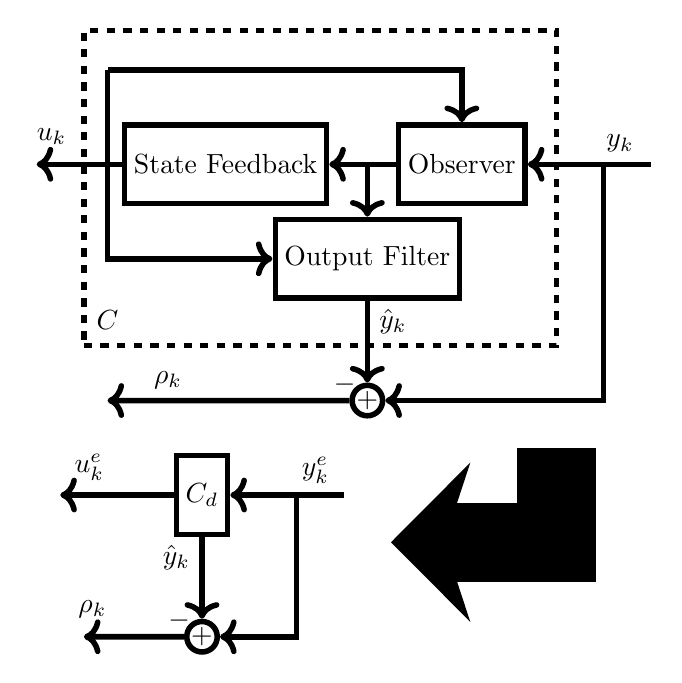
\begin{tikzpicture}[scale=0.6, every line/.style={scale=0.6}]
    % Left schematic
    \node[draw, line width = 2, rectangle, minimum height=1cm] (state) at (-3,0) {State Feedback};
    \node[draw, line width = 2, rectangle, minimum height=1cm] (observer) at (2,0) {Observer};
    \node[draw, line width = 2, rectangle, minimum height=1cm] (delay) at (0,-2) {Output Filter};
    \node[draw, line width = 2, circle, inner sep=0.01cm, minimum width=0.1cm, minimum height=0.1cm] (plus) at (0,-5) {+};
    
    \draw[line width=2, ->] (6,0) -- node[pos=0.25,above] {$y_k$} (observer);
    \draw[line width=2, ->] (observer) -- (state);
    \draw[line width=2, ->] (state) -- node[yshift=10,xshift=-10] {$u_k$} (-7,0);
    \draw[line width=2, -] (-5.5,0) -- (-5.5,2);
    \draw[line width=2, ->] (-5.5,2) -| (observer);
    \draw[line width=2, ->] (0,0) -- (delay);
    \draw[line width=2, ->] (delay) -- node[pos=0.85, left,yshift=-5] {$-$} node[pos=0.25,right] {$\hat y_k$} (plus);
    \draw[line width=2, ->] (5,0) |- (plus);
    \draw[line width=2, ->] (-5.5,0) |- (delay);
    \draw[line width=2, ->]  (plus) -- node[pos=0.75, above] {$\rho_k$} (-5.5,-5);

    \node[draw, line width = 2,rectangle,fill=none,dashed, minimum width=6cm, minimum height=4cm] at (-1,-0.5) {};

    \node at (-5.5,-3.3) {$C$};

    \draw[line width=2, -{Stealth[length=10mm, width=20mm]}, black ,line width=10mm] (4,-6) |- (0.5,-8);
    
    % Right schematic
    \begin{scope}[xshift=-3.5cm,yshift=-7cm]
        \node[draw, line width = 2, rectangle, minimum height=1cm] (state) at (0,0) {$C_d$};
        \node[draw, line width = 2, circle, inner sep=0.01cm, minimum width=0.1cm, minimum height=0.1cm] (plus) at (0,-3) {+};
        %\node[draw, line width = 2, rectangle, minimum height=1cm] (scale) at (2,-1.5) {$c^{\bar k}$};
        
        \draw[line width=2, ->] (state) -- node[yshift=10,xshift=-10] {$u^e_k$} (-3,0);
        \draw[line width=2, ->] (3,0) -- node[pos=0.25,above] {$y_k^e$} (state);
        \draw[line width=2, ->] (state) -- node[pos=0.85, left,yshift=-5] {$-$} node[pos=0.25,left] {$\hat y_k$} (plus);
        \draw[line width=2, ->]  (plus) -- node[yshift=10,xshift=-15] {$\rho_k$} (-2.5,-3);
        \draw[line width=2, ->] (2,0) |- (plus);
        %\draw[line width=2, ->] (2,0) -- (scale);
    \end{scope}
\end{tikzpicture}
    \caption{Instead of individually converting each block in the controller to be compatible with encrypted signals, we reduce the compounding approximation errors by combining the three blocks (two static and one dynamic) into a single dynamic block, $C_d$ with two outputs. It is made compatible with integer signals by scaling and rounding its parameters.% To ensure correct comparisons, the unfiltered signal is scaled with $c^{\bar k}$.
    }    \label{fig:controller_enc_fig}
\end{figure}
Furthermore, as we saw in Lemma~\ref{lem:ishomomorphic}, additions and multiplications increase the variance of the injected noise during encryption. Implementing controllers over encrypted signals should, therefore, ideally, minimize the number of computational steps to avoid a potential detour into numbers below the precision limit or deterioration of the result due to the increase in noise. Controllers and detectors in the traditional encrypted-free setting contain internal loops and are split up into multiple steps, which is shown in the top part of Fig.~\ref{fig:controller_enc_fig}. For the encrypted setting, it is beneficial if as few operations as possible are done. In this paper, we will aggregate the operations into a single transformation, depicted in the bottom part of Fig.~\ref{fig:controller_enc_fig} as $C_d$. However, $C_d$ will still have an internal state variable, meaning that internal loops within it are not fully removed.
% In the encryption-free setting, controllers and detectors can run independently since the number of additions and multiplications performed on the samples does not deteriorate the result. As a result, a controller typically contains several internal loops, and the computation of signals is split into multiple steps, as shown in the top part of Fig.~\ref{fig:controller_enc_fig}. For the encrypted setting, however, we must consider the noise amplification every time addition or multiplication is performed~\cite{}. Particularly, it is beneficial if as few operations as possible are done. In this paper, we will aggregate the operations into a single transformation, depicted in the bottom part of Fig.~\ref{fig:controller_enc_fig} as $C_d$. However, $C_d$ will still have an internal state variable, meaning that internal loops within it are not fully removed.
%, which will be evident in Section~\ref{sec:hyptest}. 
% We shall return to how to realize such controllers in Section~\ref{sec:controllers}. For now, we will only state the following idea, which is vital for enabling detection over control: we use the \emph{controller's} observer for detection. Instead of using the input signal that the controller produces, $u_k$, and running it through \emph{another} observer, we directly connect to the controller's observer and extract a signal from there to be used in the detection, thus substantially reducing the number of operations performed on the signals. 
% Furthermore, the LWE encryption scheme only works over integers, meaning real numbers must be mapped to integers. In this paper, the mapping is realized with a dynamic scaling factor $c^{\bar k} \in \mathbb Z$. We show two possible controllers and detectors co-design schemes in Section~\ref{sec:controllers}. But for now, we shall only state that the controller also computes an estimated encrypted output 
% operating over encrypted data requires modifications to the controllers since encryption only works over integers, which we shall also see in Section~\ref{sec:controllers}. The controllers we design will output the following signal, whose computation will have the following form, which we state as an assumption for now:
% \begin{asm}\label{asm:controller_estimates_output}
%     The encrypted output of the plant $y^e_k$ is estimated by the controller based on its internal state $x_k^c$ and a sequence of past measurements, $$\hat{y}^e_k = C_ex_k^c+D_e\begin{bmatrix}
%         y_0^e \\ \vdots \\ y_{k-1}^e
%     \end{bmatrix},$$
% where $C_e$ and $D_e$ are matrices with integer elements.
% \end{asm}
% Assumption~\ref{asm:controller_estimates_output} does not limit control performance since more states that do not affect the control signal $u_k^e$ can be added to the controller, which will be seen in Section~\ref{sec:controllers}. Additionally, the choice of the controller we consider does not impact our main result as long as the controller can be made compatible with integer signals and can output an estimation of the output based on its internal state, see Point~\ref{point:detect} below.
The estimated output of the plant $y^e_k$ based on its internal state $x_k^c$ and a sequence of possibly corrupted past measurements can be written as
\begin{equation}\label{eq:controller_estimates_output}
         \hat{y}^e_k = C_ex_k^c+D_e\begin{bmatrix}
        \tilde y_0^e \\ \vdots \\ \tilde y_{k-1}^e
    \end{bmatrix}
    \end{equation}
where $C_e$ and $D_e$ are matrices with integer elements.%, $c \in \mathbb Z_+$ is an integer scaling factor, and $\bar k \in \mathbb Z_+$ is a periodic function of $k$.

Equation~\ref{eq:controller_estimates_output} does not limit control performance since the extra signals that the controller outputs do not affect the encrypted input signals, $u_k^e$. Thus, as long as the controller can be cast in a compatible integer formulation, we can add an extra output using the computation it already makes.

% However, the estimated output $\hat y^e_k$ will always be scaled with some constant that we denote as $c^{\bar k}$, where $\bar k$ will depend on the type of controller we implement. 
The filtered signal $\hat y^e_k$ in Equation~\ref{eq:controller_estimates_output} will also be scaled dynamically with another quantization factor, which we will see in Section~\ref{sec:controllers}, related to the \emph{multiplication depth} of the cryptosystem. The estimated output $\hat y^e_k$ must match the scaling of $\tilde y^e_k$ to create a residual. For now, we shall say this scaling is done implicitly. %since our LWE-based cryptosystem does not support division as a homomorphism, which would give us the unscaled signal $\hat y^e_k$, the only option is to scale $\tilde y_k^e$ instead. 
The anomaly detector looks, therefore, at the following encrypted residual,
\begin{equation}\label{eq:encrypted_residual} 
    \rho_k^e = (\tilde y^e_k-\hat{y}_k^e) \bmod q,
\end{equation}
where $\tilde y_k^e =  y^e_k+y^a_k$, to detect an attack. %When the system is not under attack, the plaintext version of the residual should output a stream of zeros. Recall that we concluded in Chapter~\ref{ch:PrelimAttackEnc} that the attacker never reveals what the individual sampled signals or input-output trajectories are. Rather, they use linear combinations of trajectories to figure out the underlying signal's dynamics. And since any linear combinations of a zero signal should also be zero, the anomaly detector only needs to test whether the residual dynamics in~\eqref{eq:encrypted_residual} are zero and the sum is zero.
We model an attacker that can additively inject signals $u^a_k$ and $y^a_k$ onto the actuators and sensors, respectively. During a disclosure phase, the attacker can also read the signals $y^e_k$ and $u^e_k$ and generate attacks based on them using an algorithm the defender does not know about. It is possible that an attacker can learn \emph{undetectable} attacks from the data~\cite{taheri2021,alisic2021ecc}, which implies that $\rho_k=0, \, \forall k$. See Definition 1 and Lemma 3.1 in~\cite{Pasqualetti2013} for a definition of undetectable attacks. However, to make our analysis tractable, we require that the attacks can be detected.
\begin{asm}\label{asm:detectable}
% The attacker only injects attack signals that are \emph{detectable} in the non-encrypted setting.
The attacker injects detectable attacks. Specifically, the attacks occasionally make $\rho_k \neq 0$.
\end{asm}
% Through Assumption~\ref{asm:detectable}, we assume that the attacker changes signals so that statistical inconsistencies arise in the signals on the controller side in an unencrypted setup. These can then be used for detection.
Solving the following problem enables detection.
\begin{prob}\label{prob:main}
    Consider the following two hypotheses:
    \begin{itemize}
        \item $\mathcal{H}_0:$ $\dec^\lambda_s( \rho_k^e)=0$, $\forall k$,
        \item $\mathcal{H}_1:$ $\dec^\lambda_s( \rho_k^e)\neq 0$ for some time steps $k$.
    \end{itemize}
    Without using the secret vector $s$, how can $\mathcal{H}_0$ be rejected in favor of $\mathcal{H}_1$ with a specific probability $\alpha$ on the Type~I Error?
\end{prob}

In plain detection terminology, Problem~\ref{prob:main} asks how to detect anomalies in encrypted signals with a set false alarm rate. We decouple the problem of detection \emph{given} a residual signal, from the control-theoretic aspects of obtaining the residual. Furthermore, the residual signal is rarely always zero as in $\mathcal{H}_0$. Even in a deterministic setting, small and sparse errors are introduced due to the quantization of the signals. An example would be limit cycles for the control of unstable plants. We shall therefore also seek to detect attacks under such scenarios:
\begin{prob}\label{prob:secondary}
    Consider the following two hypotheses:
    \begin{itemize}
        \item $\mathcal{H}_0^e:$ $\Vert \dec^\lambda_s( \rho^e)\Vert _\infty \leq \epsilon_\infty$ and $\Vert \dec^\lambda_s( \rho^e)\Vert_0 \leq \epsilon_0$,
        \item $\mathcal{H}_1^e:$ $\Vert \dec^\lambda_s( \rho^e)\Vert _\infty > \epsilon_\infty$ or  $\Vert \dec^\lambda_s( \rho^e)\Vert _0 > \epsilon_0$,
    \end{itemize}
    where $\rho^e= \begin{bmatrix}\left(\rho_1^e\right )^\top & \dots & \left(\rho_N^e \right)^\top \end{bmatrix}^\top$. Without using the secret vector $s$, how can $\mathcal{H}^e_0$ be rejected in favor of $\mathcal{H}^e_1$ with a false alarm probability $\alpha$?
\end{prob}

At first glance, Problem~\ref{prob:secondary} seems to be a mere attempt at error-handling for potentially sparse errors. However, it should be viewed as the \emph{controller's impact on detection strength}, a relatively novel idea in detection literature. By proposing a mechanism that solves the hypothesis tests, we can determine which characteristics of the residual are necessary for detection. Furthermore, we will also observe how these characteristics affect detection strength, which can be used to design controllers. However, we will save the design problem for future work.
% \emph{detection} problem from the \emph{computation} of the residual by incorporating the computational part into the controller, where the effect of the expected response of the plant based on the input $u$ is computed directly. 
The rest of the paper is organized to solve these two sub-problems:
\begin{itemize}
    \item \label{point:detect} \emph{Detection}: We develop a theory that allows us to perform a hypothesis test on encrypted signals and solve Problems~\ref{prob:main} and~\ref{prob:secondary} given access to the residual \eqref{eq:encrypted_residual}.
    \item \emph{Characteristics}: We show what characteristics from the residual must be known to perform detection and how those characteristics affect the detection strength.
\end{itemize}
The detection problem will partially utilize tools found in the cryptography community, such as searching for short vectors in a lattice. In contrast, we will use control-theoretic tools to obtain the characteristics of the residual signal.

% \begin{rem}
% There is a subtle difference between Problem~\ref{prob:main} and the LWE problem. In essence, the decision version of the LWE problem is solved if one can \emph{reject $\mathcal{H}_1$ in favor of $\mathcal{H}_0$}, which is a different problem compared to Problem~\ref{prob:main}. If $\mathcal{H}_1$ could be rejected, then the secret vector would be recoverable by modifying the encrypted messages and looping through possible keys, element by element, see Lemma 4.2 in~\cite{regev2009}.
% \end{rem}

% In some conventional anomaly detection setups, such as in~\cite{Umsonst2022}, the anomaly detector carries its own internal observer for reconstructing the output or residual. We have chosen a more integrated approach through Assumption~\ref{asm:controller_estimates_output}. The reason is two-fold:
% \begin{enumerate}
%     \item Reduce noise amplification: In the conventional setup, the calculated control signal $u^e_k$ would have to be run through \emph{another} estimator, which would both further amplify the noise and add another layer of dynamical states that may need to reset more often.
%     \item \label{point:detect} Separate \emph{detection} from \emph{estimation}: We can focus the discussion on \emph{detecting} that the measured encrypted output $y^e_k$ deviates from the expected encrypted output $\hat{y}^e_k$, no matter how we obtain $\hat y_k^e$.
% \end{enumerate}

% We essentially encode an output predictor directly into the controller by using its control law, $\hat y^e_k = K(s)y^e_k$ where $K(s)=P(s)C(s)$, instead of taking the extra step of first computing the input signal $u^e_k$ and then predicting $\hat y_k^e=P(s)u^e_k$. We can then create a residual with one final operation by subtracting the prediction from the encrypted measurements to form a signal that should be constantly zero under no attacks.

\section{Main Results}\label{sec:results}

% Let us return to the case of bypassing encryption for detection purposes, which is different from bypassing encryption for estimation. 
% We shall now consider a method to bypass the encryption. It is a simplified version of the one reported in~\cite{alisic2023modelfreelwe}, since the dynamics of the signals in this paper \emph{should} constantly be zero in the unattacked case. Essentially, our approach is to remove the $Ps$ terms from the samples. 
We shall now consider the first method we need for detection. It was first reported in~\cite{alisic2023modelfreelwe} as part of a method to bypass the encryption when learning attacks. In particular, consider the encrypted residual messages from~\eqref{eq:encrypted_residual}:
\begin{equation*} 
    \enc^\lambda_s(\rho_k) = (P_k^\rho, P_k^\rho s+r\rho_k+e_k^\rho) \bmod q.
\end{equation*}
where we have redefined $P_k^\rho= (P_k^y-P_k^{\hat y}) $ and $\rho_k= (\tilde y_k-\hat y_k)$ for brevity. We will start by ``filtering out" the part that depends on the secret vector, $P_k^\rho s$, by finding linear combinations of encrypted messages that remove it.% analogously to~\eqref{eq:firstglancefilter}.

Finding such a \emph{filtering vector} $d$ can be done algorithmically by computing the corresponding $q$-ary lattice for the matrix comprised of vectorized matrices $P_k^\rho$ stacked as columns in
\begin{equation} \label{eq:matrix_public_vectorized}
    \mathcal{P}^\rho= \begin{bmatrix}
        \vecc P_0^\rho & \vecc P_1^\rho &\cdots & \vecc P_{N-1}^\rho \end{bmatrix}.%\begin{bmatrix}
        %\vecc P_0^\rho & \vecc P_1^\rho &\cdots & \vecc P_{N-1}^\rho \\
        %\vecc P_1^\rho & \vecc P_2^\rho&  \cdots & \vecc P_{N}^\rho \\
        %%\vdots & \vdots & \ddots & \vdots \\
        %\vecc P_{L-1}^\rho & \vecc P_{L}^\rho & \cdots %& \vecc P_{N+L-2}^\rho 
    %\end{bmatrix}.
\end{equation}
The filtering vectors $d$ define the points that belong to the $q$-ary lattice associated with~\eqref{eq:matrix_public_vectorized}, namely, $d \in \Ker_q {\mathcal{P}^\rho}$. 
% are therefore the vectors between the origin and points in the $q$-ary lattice defined by the vectors $\Ker_q \mathcal{P}^\rho$.
% The filtering vector is then such that $d^\top \mathcal{P}^\rho \bmod q = 0$.
There will typically be $N-pv$ such vectors when $N$ is large. %To obtain these filtering vectors algorithmically, consider Algorithm~\ref{alg:HNF}, which computes the HNF of a generic matrix $V$. By letting $V=\mathcal{P}^\rho$, the set of filtering vectors $d$ are spanned by the last $N-Lpv$ column vectors of matrix $W$, which Algorithm~\ref{alg:HNF} returns together with the HNF $H$.


%\begin{algorithm}
%\caption{Computing the Hermite Normal Form of an integer matrix $V$}
%\begin{algorithmic}[1]
%\REQUIRE An integer matrix $V$ of size $m \times n$
%\ENSURE A pair of matrices $(H, W)$ such that $H$ is the Hermite Normal Form of $V$, $W$ is an $n \times n$ integer orthogonal matrix, and $VW = H$
%\STATE \textbf{Assumptions:} $n \geq m$
%\STATE Initialize $H \gets V$ and $W \gets I_n$, where $I_n$ is the identity matrix of size $n$
%\FOR{$i \gets 1$ to $m$}
%  \STATE Find the greatest common divisor in the last $k \geq i$ elements of the $i$-th row of $H$, say $h_{ik}$
%    \STATE Find the linear combination of the numbers in last $k \geq i$ elements of the $i$-th row of $H$ that equals $h_{ik}$
%    \STATE Replace the $j$-th column in $H$ with the same linear combination of column vectors, where $j$ is the smallest index of the vectors used in the linear combination
%    \STATE Replace the $j$-th row in $W$ with the linear combination of row vectors
%  \STATE Swap the $k$-th and $j$-th columns of $H$, and the $k$-th and $j$-th rows of $W$
%\ENDFOR
%\STATE Return $(H, W)$
%\end{algorithmic}
%\end{algorithm}

% Due to the homomorphic property, we can perform the linear combinations.
% \begin{equation*} 
%     \sum \limits_{k} \rho^e_k\xi_k \text{ mod } q = \sum \limits_k P_k^\rho s \xi_k + \sum \limits_k (\rho _kr+e_k^\rho)\xi_k \text{ mod } q,
% \end{equation*}
% for $\xi_k\in \mathbb{Z}_q$. Since the anomaly detector also has access to the public matrices, $P^\rho_k$, they can find weights $\xi_k$ so that:
% \begin{equation*} 
%     \sum \limits_k P_k^\rho \xi_k \bmod q = 0.
% \end{equation*}

Multiplying such a filtering vector $d=\begin{bmatrix} d_1 & d_2 & \dots \end{bmatrix}^\top$ with the residuals $\rho^e$, modulo $q$, gives
\begin{equation} \label{eq:filtered_ensemble}
    \begin{aligned}
      d^\top \rho^e \bmod q  &= (0, \sum \limits_k (\rho _kr+e_k^\rho)d_k \bmod q) \\
    & = (0, r d^\top \rho + d^\top e^\rho) \bmod q \\& = (0, r d^\top \rho + d^\top e^\rho),
    \end{aligned}
\end{equation}
where we have assumed for the last equality that $\vert r d^\top \rho + d^\top e^\rho \vert \leq \frac{q}{2}$. 
The noise term in~\eqref{eq:filtered_ensemble}, $d^\top e^\rho$, obscures the combined plaintext sum of messages, $r d^\top \rho$, thus ensuring the confidentiality of individual samples. We can state the following proposition thanks to Assumption~\ref{asm:noise_var}.
\begin{prop} \label{prop:error_dist}
The error vector $e^\rho$ from the residuals is statistically close to the zero-mean discrete Gaussian, $e^\rho \sim \mathcal{N}_{\mathbb{Z}_q}(0,\Sigma_\rho)$, for some covariance matrix $\Sigma_\rho$.
\end{prop}
\begin{proof}
    The result follows from choosing a level of the noise so that Assumption~\ref{asm:noise_var} holds, Lemma~\ref{lem:ishomomorphic}, and that we have only considered linear combinations when computing the residual in~\eqref{eq:controller_estimates_output}, which we for now denote by the matrix $T_c$.
    % the first three rows of the controller~\eqref{eq:integer_controller}, that~\eqref{eq:static_controller} only is composed by linear operations, and~\eqref{eq:encrypted_residual}. %The state reset in~\eqref{eq:integer_controller} implies that $\Sigma_\rho$ will have a repeated block-diagonal structure.
\end{proof}

% The proof for the static controller is carried out analogously, by showing that all operations are linear and producing a covariance matrix $\Sigma_\rho$.
The resulting covariance matrix $\Sigma_p$, depends on the operations done to the signal due to the controller, which we write as $\Sigma_p=\sigma^2T_c^\top T_c$. It's precise formulation will be explicitly derived in Section~\ref{sec:controllers}. Knowing $T_c$ is important here, as it is integral to the detection algorithm. In particular, Proposition~\ref{prop:error_dist} leads us to the following result.
\begin{cor}~\label{cor:distribution_residual_weighted}
    The non-zero message in~\eqref{eq:filtered_ensemble} is distributed as a discrete normal, $d^\top\rho^e \bmod q =(0,X)$, where:
    \begin{equation}\label{eq:normal}
         X \sim \mathcal{N}_{\mathbb{Z}_q}(rd^\top \rho, d^\top \Sigma_p d),
    \end{equation}
    within a statistical distance $\mathcal{O}(\epsilon)$ if $\Vert T_c^\top d\Vert_2^2 \eta_\epsilon^2(\mathbb L) \leq \sigma^2$.
\end{cor}

Corollary~\ref{cor:distribution_residual_weighted} shows us how to perform the hypothesis test we posed in Problem~\ref{prob:main}, where we assumed the ideal case of a plaintext residual being zero at all times:
\begin{thm}\label{thm:main_theorem_rejection_rule}
    Rejecting $\mathcal{H}_0$ when $ \vert X \vert \geq \gamma$, where $d^\top\rho^e \bmod q =(0,X)$ and $\gamma$ is the $\alpha$-quantile of $\mathcal{N}_{\mathbb{Z}_q}(0,d^\top \Sigma_p d)$,
    \begin{equation}  \label{eq:false_alarm_triggering_rule}
    \mathrm{Pr}(\vert Y \vert\geq \gamma)=\alpha, \quad \text{for } Y \sim \mathcal{N}_{\mathbb{Z}_q}(0,d^\top \Sigma_p d),
    \end{equation}
    produces a Type~I Error with probability $\alpha$ with a small statistical distance of $\mathcal{O}(\epsilon)$ if $\Vert T_c^\top d\Vert_2^2 \eta_\epsilon^2(\mathbb L) \leq \sigma^2$.
\end{thm}

\begin{proof}
Recall that the Type~I Error is defined as $\mathrm{Pr} (\text{Reject } \mathcal{H}_0 | \mathcal{H}_0 \text{ is true})=\alpha$. Thus, we have to construct a rejection mechanism with this property. Hypothesis $\mathcal{H}_0$ implies that $d^\top \rho=0$, which according to Corollary~\ref{cor:distribution_residual_weighted}, implies that:
    \begin{equation*} 
        X \sim \mathcal{N}_{\mathbb{Z}_q}(0, d^\top \Sigma_p d).
    \end{equation*}
    Consider the random variable $Y\sim \mathcal{N}_{\mathbb{Z}_q}(0, d^\top \Sigma_p d)$ and the sets $\mathcal{S}_i$, for which $\mathrm{Pr}(Y\subset \mathcal{S}_i)=\alpha$. Multiple such sets may exist, but we choose to use $\mathcal{S}_0={Y: Y<-\gamma, \text{ or }  Y > \gamma}$, for some $\gamma\in \mathbb{Z}_q$. Thus, we have that $\mathrm{Pr}(|Y|\geq \gamma)=\alpha$. Since $d^\top\rho^e \bmod q=X$ has the same distribution as $Y$ under $\mathcal{H}_0$, we have that: $$\mathrm{Pr}\left (\left. |X|\geq \gamma \right \vert \mathcal{H}_0 \text{ is true} \right )=\alpha,$$ which concludes our proof.
\end{proof}
\begin{rem}
    Several rejection rules that solve Problem~\ref{prob:main} appear in the proof of Theorem~\ref{thm:main_theorem_rejection_rule}, quantified by the number of sets $\mathcal{S}_i$ we can choose from. These sets are equivalent to how we could pick different rejection regions in Section~\ref{sec:hyptest}. The one we use in Theorem~\ref{thm:main_theorem_rejection_rule} is the \emph{uniformly most powerful unbiased} $\alpha$-level test~\cite{Lehmann2005}.
\end{rem}

To extend the detection mechanism to solve Problem~\ref{prob:secondary}, we return to the last line of~\eqref{eq:filtered_ensemble}, where the plaintext residual is given by $rd^\top \rho$. Since the detector does not know $\rho$, we take a worst-case approach to $\rho$'s values, even if the vector is sparse. We shall therefore approximate:
\begin{equation*}
    rd^\top \rho \approx r Y, \text{ where } Y\sim\mathcal{U}_{\epsilon_\infty \Vert d_{\epsilon_0} \Vert_1},
\end{equation*}
where $d_{\epsilon_0}$ is a vector consisting of $d$'s $\epsilon_0$ largest values. The motivation is as follows, if it is known that $\Vert \rho \Vert_0 \leq \epsilon_0$, then the largest values $d^\top \rho$ can take is $\pm \epsilon_\infty \Vert d_{\epsilon_0} \Vert_1$. In case there is no sparsity, $\epsilon_0 = Np$, then $d_{\epsilon_0}=d$. With this approximation of the error, we have:
\begin{prop}\label{prop:prop_rejection_rule}
    Rejecting $\mathcal{H}^e_0$ when $  X \in \mathcal{S}$, where $d^\top\rho^e \bmod q =(0,X)$ and $\mathcal{S}$ is a set where $\mathrm{Pr}(Y \in \mathcal{S})=\alpha$ for the random variable $Y$ with the following density function
    \begin{equation*}
        \mathrm{Pr}(y=Y) = \frac{1}{1+2 \epsilon_\infty \Vert d_{\epsilon_0} \Vert_1} \sum \limits_{k=-\epsilon_\infty \Vert d_{\epsilon_0} \Vert_1}^{\epsilon_\infty \Vert d_{\epsilon_0} \Vert_1} \mathrm{Pr}(y-kr=X),
    \end{equation*}
    % \begin{equation}  \label{eq:false_alarm_triggering_rule}
    % \mathrm{Pr}(\vert Y \vert\geq \beta)=\alpha, \quad \text{for } Y \sim \mathcal{N}_{\mathbb{Z}_q}(0,d^\top \Sigma_p d),
    % \end{equation}
    where $\mathrm{Pr}(x=X)$ is the density function for $\mathcal{N}_{\mathbb{Z}_q}(0,d^\top \Sigma_p d)$, produces a Type~I Error with probability $\alpha$ with a small statistical error of $\mathcal{O}(\epsilon)$.
\end{prop}
\begin{proof}
    Since $r d^\top \rho + d^\top e^\rho$ is a sum of a random variable sampled from a discrete normal distribution (up to $\mathcal{O}(\epsilon)$ statistical distance) and a random variable that we approximate as uniformly distributed, $\mathcal{U}_{\epsilon_\infty \Vert d_{\epsilon_0} \Vert_1}$, One can obtain the resulting density function by computing the convolution between the two density functions. 
\end{proof}
Similarly to the proof in Theorem~\ref{thm:main_theorem_rejection_rule}, multiple sets $\mathcal{S}$ may exist. One obtains the \emph{uniformly most powerful} $\alpha$-level test by picking $\mathcal{S}$ with the largest cardinality. While the largest set in the error-free case consists of points far away from the origin, the same may not hold for the case when there are errors.

Theorem~\ref{thm:main_theorem_rejection_rule} and Proposition~\ref{prob:secondary} gives rules for performing a hypothesis test once some vector $d$ has been found. %Finding multiple such vectors can be done since they come out as a by-product of converting the stacked public matrix $\mathcal{P}=\begin{bmatrix}
    %(\text{Vec}(P^\rho_1))^\top & \dots & (\text{Vec}(P^\rho_N))^\top
%\end{bmatrix}^\top$ to its HNF $H_{\mathcal{P}^\top}$, which can be obtained with a algorithm of polynomial complexity. 
While the hypothesis test depends on obtaining good filtering vectors $d$ on the cryptographic side of the problem, $d$ essentially only scales the difficulty of performing the test and a new $d$ will be obtained once a new sample is introduced into the problem. In particular, the error variance $d^\top \Sigma_\rho d$ of the discrete normal variance is scaled quadratically with $d$, and its $\epsilon_0$ largest values linearly scale the impact of quantization errors. In contrast, the system parameters $\Sigma_p$, $\epsilon_\infty$ , and $\epsilon_0$ from the control-theoretic side determine the system's best-case detection capabilities.
% This can be seen from the $\Vert d\Vert_ 2^2$ scaling of the discrete normal variance $d^\top \Sigma_\rho d$, the number of elements in $d_{\epsilon_0}$ and the $\Vert \Vert_1$ scaling
% The filtering vectors quadratically scale the error variance $d^\top \Sigma_\rho d$, but the sum $d^\top \rho$ only linearly. Therefore, if $\mathcal{H}_1$ is true and $\Vert d \Vert_2$ is large, then $d^\top \rho$ would also need to be large to trigger an alarm. It is difficult to make $d^\top \rho$ large since we do not know $\rho$. One approach is to recognize the temporal nature of $\rho$, namely that only recently sampled residuals will be non-zero after an attack starts. So, $\rho_k=0$ for $k={1, \, \dots, \, N-l}$, and $\rho_k\neq 0$ for $k={N-l+1, \, \dots, \, N}$, for some $l \ll N$.

We also need to recognize the temporal nature of the problem. It is most valuable if anomaly is detected in the \emph{most recent samples}. The samples that are ignored are encoded in the filtering $d$ through its elements that are zero. Therefore, we want to ensure that the most recent samples are used in the detection scheme. Therefore, we want the filtering vector $d$ to have the following two properties:
\begin{enumerate}
    \item Structured: The first elements in $d$ should be 0 so that only recent samples are used for detection.
    \item Short: The norms $\Vert d_{\epsilon_0} \Vert_1$ and $\Vert d\Vert_2$ should be small to reduce error amplification.
\end{enumerate}
In Section~\ref{sec:vectors}, we show that these two properties can oppose each other and that a trade-off between them has to be considered.

% \begin{rem}
%     The large variance scaling stops the detector from solving the LWE problem. If $e^\rho=0$ and $\rho=0$, the detector would be able to guess secret vectors and use $d^\top \rho^e \bmod q=0$ to verify the correct guesses, see~\cite{regev2009}. The detection rule in Theorem~\ref{thm:main_theorem_rejection_rule} does not conclude that $d^\top \rho^e \bmod q \approx d^\top \rho=0$, instead it asks when $d^\top \rho^e \bmod q$ it is sufficiently large to conclude that $d^\top \rho \neq 0$.
% \end{rem}

\section{Hypothesis Testing under LWE}\label{sec:hyptest}
The proposed detection scheme seems, at first glance, like it violates the security properties of LWE, in particular since we still are dependent on finding a short vector. In this section, we will clarify the difference between the two problems, and show that the problem related to detection actually scales polynomially with the length of the shortest vector, as opposed to exponentially. Hypothesis tests are used to exemplify the hardness of the LWE problem in the original work by Regev~\cite{regev2009}. In particular, it is shown that if an efficient algorithm can reject that a set of samples comes from the uniform distribution in favor of a so-called \emph{LWE distribution}, see Definition~\ref{def:lwedist} below, then the secret vector $s$ can also be recovered efficiently. However, the existence of such a rejection algorithm would imply that the LWE problem is easy to solve. Let us now define what we mean by the LWE distribution.

The uniform distribution $\mathcal{U}_q$ can be combined with the discrete normal distribution from Definition~\ref{def:discretenormal} to make the LWE distribution as follows.
\begin{defi} \label{def:lwedist}
A sample from the LWE distribution $\mathcal{L}_{v,q,\sigma^2}(s)$ with parameters $v$, $q$, and $\sigma^2$ is defined as a tuple, $(P,b)$, where the elements of $P \in \mathbb Z_q^{v}$ are sampled from $\mathcal{U}_q$, and $b$ is given by,
\begin{equation*}
    b \coloneqq Ps+e \bmod q,
\end{equation*}
where $e \sim \mathcal{N}_{\mathbb{Z}_q}(0,\sigma^2)$. The vector $s \in \mathbb Z_q^v$ parametrizes the specific LWE-distribution.
%The LWE distribution with parameters $n,q,s$, $\mathcal{L}_{n,q,s}$, is defined over the finite support $\mathbb Z_q^v \times Z_q$, and its probability distribution is given by
%\begin{equation*}
%\mathrm{Pr}((\mathbf{a},b)=(\mathbf{p},\mathbf{p}\cdot\mathbf{s}+\mathbf{e}) \bmod q) = \frac{1}{|\mathcal{S}|}\phi(\mathbf{e}), \quad \text{for } (\mathbf{a},b) \in \mathbb{Z}_q^n \times \mathbb{Z}_q,
%\end{equation*}
%where p is a vector sampled from the discrete uniform distribution US, e is a scalar sampled from the discrete normal distribution $Nd(0,s2)$, and s is a fixed secret vector in Zqn.
\end{defi}

Comparing to the encryption scheme in Definition~\ref{def:lwe}, and specifically~\eqref{eq:lweencmsg}, one can see that a sample from the LWE distribution is the same as encrypting the plaintext message $m=0$. In particular, we can identify the null hypothesis $\mathcal{H}_0$ in Problem~\ref{prob:main} as being equivalent to having a collection of samples from the LWE distribution,
\begin{itemize}
    \item $\mathcal{H}_0$: $\rho_k^e\sim \mathcal{L}_{v,q,\sigma^2}(s)$, $\forall k$.
\end{itemize}

The test we used in Section~\ref{sec:results} finds integer-linear combinations of messages so that the result, after modulo $q$, removes the explicit dependence on $P_k^\rho$,
\begin{equation*}
    d^\top \rho^e \bmod q = (0, d^\top e \bmod q).
\end{equation*}
Now, if the result is sufficiently small, namely if $\vert d^\top e \vert < \frac{q}{2}$, we will have an integer-linear combination of samples distributed as discrete normal which, thanks to Assumption~\ref{asm:noise_var}, is also distributed ($\epsilon$-close) as a discrete normal, see~\cite{boneh2011}. Therefore, we can convert the null hypothesis to:
\begin{itemize}
    \item $\mathcal{H}_0$: $d^\top \rho^e \bmod q = (0,X)$, where $X\sim \mathcal{N}_{\mathbb{Z}_q}(0,\Vert d\Vert_2^2\sigma^2)$. 
\end{itemize}
In other words, the null hypothesis is that $X$ is sampled from the discrete normal distribution.

Consider now the alternative hypothesis $\mathcal{H}_1$, which assumes that (at least some of) the plaintext residual samples are non-zero. Performing the same integer-linear combination of samples yields
\begin{equation}\label{eq:uniform_result}
    d^\top \rho^e \bmod q = (0, d^\top \rho r + d^\top e \bmod q),
\end{equation}
where $\rho$ is some strictly non-zero vector. The effect of the non-zero $\rho r$, especially if it is sufficiently large, can be understood by comparing the second tuple in~\eqref{eq:uniform_result} with the following class of pseudo-random uniform number generators, see~\cite{rotenberg60}, which outputs sequences that pass formal test of randomness, however, can be predicted if the parameters are known.

\begin{lem}\label{lem:makeUnif}
    Consider the two integers $a\in\mathbb Z_q$ and $c \in \mathbb Z_q$ for prime $q$ and let $X \sim \mathcal{U}_q$. Then, the following affine transformation:
    \begin{equation} \label{eq:uniformize}
        Y= aX+c \bmod q
    \end{equation}
    is also pseudo-uniform, $Y \sim \mathcal{U}_{q}$, if $a$ and $q$ are coprime.
\end{lem}

Essentially, the information about $a$ and $c$ is destroyed because they cannot be recovered from $Y$ even if the realization of $X$ is known. We can, therefore, identify the second tuple in~\eqref{eq:uniform_result} as a sum of pseudo-uniform random number generators with different parameters $a_k=\rho_kr$ and $c_k=d_ke_k$,
\begin{equation*}
   d^\top \rho r + d^\top e \bmod q =  \left ( \sum \limits_k d_k\rho_kr + d_ke_k \bmod q \right) \bmod q.
\end{equation*}
The final modulo operation maps the sum of pseudo-uniform random numbers over $\mathbb Z_q$ back to $\mathbb Z_q$, which follows a pseudo-uniform distribution again, as is shown next.
\begin{lem}
\label{lem:sum_pseudo_unif}    Consider a set of messages $u_k$ sampled from the uniform distribution, $u_k \sim \mathcal{U}_{q}$ and let $q$ be prime. Then, the linear combination
    \begin{equation*}
        U \coloneqq \sum \limits_k a_k u_k \bmod q,
    \end{equation*}
    where $a_k \in \mathbb Z_q$ and $a_k \neq 0$ for some $k$, is also uniform, $U \sim  \mathcal{U}_{q}$.
\end{lem}
\begin{proof}
    First, note that the sum of two uniformly distributed variables $u_i, u_j \sim  \mathcal{U}_{q}$, is also uniform after the modulus operator has been applied,
    \begin{equation*}
        u_i+u_j \bmod q \sim  \mathcal{U}_{q}, \quad \text{ if } i\neq j.
    \end{equation*}
    Secondly, multiplying a uniform number $u_k$ with an integer $a_k \in \mathbb Z_q$ is also integer,
    \begin{equation*}
        a_k u_k \bmod q \sim  \mathcal{U}_{q},
    \end{equation*}
    if $a_k \neq 0$, since $a_k$ and $q$ are coprime. The last part of the proof follows from recurrence. Let us define
    \begin{equation*}
        S_{k+1} = S_k + a_{k+1}u_{k+1} \bmod q, \quad S_1 = a_1u_1 \bmod q.
    \end{equation*}
Note that since $S_k$ and $a_{k+1}u_{k+1} \bmod q$ are both uniform, then their sum modulo $q$, $S_{k+1}$, is uniform too.
\end{proof}

% {\color{red} Rewrite H1 here. Then let discussion on Regev commence!}

The uniformity of~\eqref{eq:uniform_result} allows us to reformulate Problem~\ref{prob:main} into the following one, which is the problem we solve when performing anomaly detection.
\setcounter{prob}{1}
\begin{subprob} \label{prob:reworked_prob}
    Consider the following two hypotheses:
    \begin{itemize}
        \item $\mathcal{H}_0$: $d^\top \rho^e \bmod q = (0,X)$, where $X\sim \mathcal{N}_{\mathbb{Z}_q}(0,\Vert d\Vert_2^2\sigma^2)$. 
        \item $\mathcal{H}_1$: $d^\top \rho^e \bmod q = (0,U)$, where $U\sim \mathcal{U}_q$. 
    \end{itemize}
    Reject $\mathcal{H}_0$ in favor of $\mathcal{H}_1$ with a specific probability $\alpha$ on the Type~I Error.
\end{subprob}



% Due to the addition of the uniform distribution of $P_k^\rho s$, the modulus operator maps any distribution back to a (pseudo-)uniform distribution, thus obfuscating the message to the point of no recovery, which we shall return to later. In principle, the elements of $s$ should also be sampled from $\mathcal{U}_q$ to reduce the probability that an attacker could guess $s$.

In the following, we shall explain the subtle difference between Problem~\ref{prob:reworked_prob} and the one treated in~\cite{regev2009}, which reveals the secret vector. % In the LWE distribution, the injected error $e_k$ is not \emph{completely} unknown. Rather, it is sampled from a known distribution. Now, 
Consider a collection of samples from the LWE distribution, denoted by $(P_k, P_k s + e_k \bmod q)$, where $k$ is a label for each sample. Then, draw an integer from the uniform distribution for each sample, $p_k \sim \mathcal{U}_{q}$ and modify each sample as follows.
\begin{align*}
    & (P_k+p_k \begin{bmatrix}
        1 & 0 & \dots & 0 
    \end{bmatrix} \bmod q, P_k s + e_k \bmod q) \\ 
    = & (\tilde P_k, P_ks +e_k +p_ks_1 -p_ks_1 \bmod q) \\ 
    = &(\tilde P_k, \underbrace{-s_1}_a \underbrace{p_k}_X + \underbrace{\tilde P_ks +e_k}_{c}  \bmod q).
\end{align*}

The last element in the transformed tuple sample can be compared to the output of the pseudo-random uniform number generator~\eqref{eq:uniformize}, where we can identify the known $p_k$ as $X$, and the unknown parameters $-s_1$ and $\bar P_k + e_k$ as $a$ and $c$, respectively. In other words, we have \emph{transformed our LWE samples into} (pseudo-random) \emph{uniform samples}.

% This transformed sample will now be uniform due to Lemma~\eqref{lem:makeUnif} because $s_1$ is unknown and can be identified as $a$, the known integer $-p_k$ is drawn from a uniform distribution similar to $X$, and $\tilde P_ks +e_k$ is unknown, similar to $c$, because of the unknown product $\tilde P_ks$.

Uncovering the first element of secret vector $s$, namely $s_1$, occurs when a transformation back to the LWE distribution is performed \emph{and verified}. In particular, first make a guess of $s_1$, which we denote as $\tilde s_1$. Then, multiply it with the known integer $p_k$, and add the product to the second part of the tuple
\begin{equation*}
    (\tilde P_k, \underbrace{(\tilde s_1 - s_1)}_a \underbrace{p_k}_X + \underbrace{\tilde P_ks +e_k}_{c}  \bmod q).
\end{equation*}
Note that the sample remains uniform if a wrong guess is made, $\tilde s_1 \neq s_1$. The only thing that changes is the (unknown) parameter $a$ in the pseudo-random number generator. However, if a correct guess is made, $\tilde s_1=s_1$, the samples will no longer be uniform. Rather, they will be LWE samples again. If there is a way to verify that the samples have been transformed back to LWE, then the (first element of the) secret vector has been revealed. Therefore, to reveal elements of the secret vector, the following problem has to be solved.
\begin{regevProblem}
    Consider the two hypotheses in Problem~\ref{prob:reworked_prob}. Reject $\mathcal{H}_1$ (Uniform) in favor of $\mathcal{H}_0$ (LWE) with a specific probability $\alpha$ on the Type~I Error.
\end{regevProblem}

If $\mathcal{H}_1$ can be rejected efficiently (polynomial complexity), then at most $q$ guesses per element of the secret vector are needed, $\mathcal{O}(qv)$, making the entire scheme polynomial.

% \begin{rem}
%     A similar setup is used in~\cite{regev2009} to prove security against chosen-plaintext attacks (CPA). In particular, if the attacker subtracts a guessed message $m'$ from the ciphertext $( P_k, P_ks +r(m-m')+e_k \bmod q)$ then it can only \emph{accept} a correct guess, $m'=m$, by rejecting $\mathcal{H}_1$ (Uniform).
% \end{rem}

% but LWE, and rejecting that the samples are uniform will confirm that the guess $\tilde s_1$ is correct. The rest of the elements of $s$ are treated analogously, and the full algorithm is summarized in Algorithm~\ref{alg:revealS}. As such, at most $q$ guesses will be needed per element of $s$, which makes the uncovering $s$ have polynomial complexity if the rejection algorithm is polynomial.

We summarize the two different problems and their implications in Fig.~\ref{fig:visual_break_LWE}. It is the verification in the second step that reveals the secret vector in~\cite{regev2009}. When we solve Problem~\ref{prob:reworked_prob} to perform anomaly detection, we verify the first step in Fig.~\ref{fig:visual_break_LWE}, which would \emph{not reveal the secret vector}. The rest of this section is devoted to showing that solving Problem~\ref{prob:reworked_prob} can be done more efficiently.

% However, to get there, one needs to transform the sample into a uniform one, which is implicitly assumed to be possible without needing confirmation. But such a transformation may fail, for instance, because $s_1=0$, which makes confirmation impossible to do and subsequently makes it harder to find the secret vector.

% The problem our detection scheme differs from the scheme that reveals $s$ in two ways: 1), it relies on confirming Step 1, as opposed to Step 2, and 2), it bypasses the encryption by removing the keys entirely instead of revealing them.  %it modifies the \emph{message} $m_k$, instead of the secret vector $s$.
% Furthermore, we perform the hypothesis test with a linear combination of all samples. Such a test is equivalent to rejecting the LWE distribution using only one sample with a different variance of $e_k$. The rejection scheme is possible if the resulting new variance of $e_k$ is sufficiently small (but not as small as required to do Step 2 in Fig.~\ref{fig:visual_break_LWE}), which we shall show next.

% {\color{red} In this paper, we shall approach the hypothesis test differently. In particular, we will design a test that rejects the LWE distribution, Step 1 of Fig.~\ref{fig:visual_break_LWE}, with only one linear combination of all samples. Such a test is equivalent to rejecting the LWE distribution, with a different variance of $e_k$, using only one sample. The rejection scheme is possible if the resulting new variance of $e_k$ is sufficiently small. Additionally, the scheme does not violate the assumption on the confidentiality of $s$, since any rejection mechanism of the uniform distribution using only one sample will result in large Type~I Error probabilities.}

% The first step to uncover the secret vector was to transform the LWE samples to uniform, which the author assumed was possible. However, the proposed transformation may fail, particularly if $s_1=0$. Confirmation that the samples have transformed to a uniform distribution, and therefore rejecting that they are LWE, will not break the LWE-based cryptosystem. In fact, it is implicitly assumed that even if such a rejection is made, and the sample becomes uniform, then the vector $s$ will still remain hidden. 

\begin{figure}
    \centering
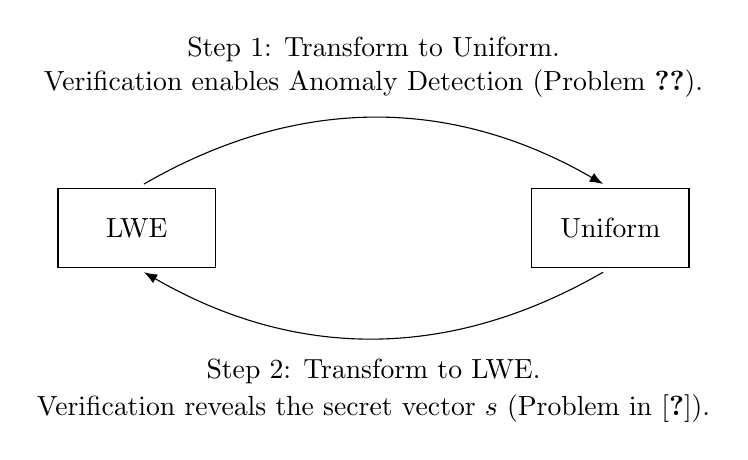
\begin{tikzpicture}[
  node distance=2cm and 4cm,
  box/.style={draw,minimum width=2cm,minimum height=1cm,align=center},
  arc/.style={-Latex,shorten >=3pt,shorten <=3pt}
  ]
  \node[box] (LWE) {LWE};
  \node[box,right=of LWE] (Uniform) {Uniform};
  \draw[arc] (LWE.north) to[bend left] node[midway, above, yshift=4ex] {Step $1$: Transform to Uniform.} node[midway, above, yshift=1ex]{Verification enables Anomaly Detection (Problem~\ref{prob:reworked_prob}).} (Uniform.north);
\draw[arc] (Uniform.south) to[bend left] node[midway, below, yshift=-1ex] {Step $2$: Transform to LWE.} node[midway, below, yshift=-4ex] {Verification reveals the secret vector $s$ (Problem in~\cite{regev2009}).}  (LWE.south);
\end{tikzpicture}    
    \caption{The schematic shows a high-level picture of how the secret vector is revealed using the algorithm laid out in~\cite{regev2009}. First, the LWE sampled is transformed into a uniform one by modifying the public key, as shown in Step 1 (confirmation that this transformation is successful is not treated in~\cite{regev2009}). Then, by guessing the correct value of the secret vector, one can return the sample back to an LWE sample, as in Step 2. The ability to confirm that the sample is LWE again verifies the guess and thus reveals the secret vector.}
    \label{fig:visual_break_LWE}
\end{figure}



% \begin{algorithm} \label{algo:revealS}
% \caption{Recovering the secret vector $s$ from LWE samples}
% \begin{algorithmic}[1]
% \REQUIRE A collection of LWE samples $(P_k, b_k)$ for $k = 1, \dots, m$
% \ENSURE The secret vector $s$
% \STATE \textbf{Assumptions:} The parameters $q$ and $v$ are known.
% \STATE \textbf{Function:} $\textsc{IsUniform}(Q)$ returns \texttt{True} if the samples in the collection of  $Q={(A_k, B_k)}$ is uniform, \texttt{False} otherwise
% \STATE Initialize an empty vector $s$ of length $v$
% \FOR{$i = 1$ to $v$}
%   \FOR{$j = -(q-1)/2$ to $(q - 1)/2$}
%     \STATE $\tilde s_i \gets j$
%     \STATE Create a new collection of samples $Q$
%     \FOR{$k = 1$ to $m$}
%       \STATE Draw a random integer $p_k$ from the uniform distribution over $[- (q - 1) / 2, (q - 1) / 2]$
%       \STATE Modify the $k$-th sample as $(P_k + p_k \delta_{il} \bmod q, b_k + p_k \tilde s_i \bmod q)$
%       \STATE Add the modified sample to $Q$
%     \ENDFOR
%     \STATE \texttt{result} = $\textsc{IsUniform}(Q)$
%       \IF{result == \texttt{False}}
%       \STATE $s_i \gets \tilde s_i$
%       \STATE Break the loop
%     \ENDIF
%   \ENDFOR
% \ENDFOR
% \STATE Return the secret vector $s$
% \end{algorithmic}
% \end{algorithm}

% \begin{algorithm} 
% \caption{Recovering the secret vector $s$}
% \begin{algorithmic}[1] \label{alg:revealS}
% \REQUIRE A collection of LWE samples $(P_k, b_k)$ for $k = 1, \dots, m$
% \ENSURE The secret vector $s$
% \STATE $s \gets 0$ of length $v$
% \FOR{$i = 1$ to $v$}
%   \FOR{$j = -(q-1)/2$ to $(q - 1)/2$}
%     \STATE $\tilde s_i \gets j$, $Q \gets \emptyset$
%     \FOR{$k = 1$ to $m$}
%       \STATE $p_k \sim \mathcal{U}_{[- (q - 1) / 2, (q - 1) / 2]}$
%       \STATE $Q \gets Q \cup {(P_k + p_k \delta_{il} \bmod q, b_k + p_k \tilde s_i \bmod q)}$
%     \ENDFOR
%     \IF{$\textsc{IsUniform}(Q)$ == \texttt{False}}
%       \STATE $s_i \gets \tilde s_i$
%       \STATE Break the loop
%     \ENDIF
%   \ENDFOR
% \ENDFOR
% \RETURN $s$
% \end{algorithmic}
% \end{algorithm}


% Consider the linear combination of a collection of samples from the LWE distribution, $(P_k, P_ks+e_k \bmod q)$, with some  %The LWE problem essentially guarantees that removing the $P_ks$ part~\emph{in a good way} from $m_k^e$ is difficult, even when $P_k$ is known. In the following, we shall exemplify why it is not easy.
% integer weights $a_i \in \mathbb{Z}_q$,
% \begin{multline*}
%     \sum \limits_{k} (P_ks +e_k)a_k \text{ mod } q \\= \sum \limits_k P_ksa_k + \sum \limits_k (m_kr+e_k)a_k \text{ mod } q.
% \end{multline*}
% Now, since $P_k$ is also broadcast, the attacker can find integers $a_k$ so that ${\sum \limits_k P_ka_k \bmod q =0,}$ which gives
% \begin{equation}~\label{eq:firstglancefilter}
% \begin{aligned}
%     \sum \limits_k (P_ks+e_k)a_k \bmod q &= (\sum \limits_k a_kP_k)s+\sum \limits_k e_ka_k \bmod q \\ 
%     &= \sum \limits_k e_ka_k \bmod q,
% \end{aligned}
% \end{equation}
% which is a noisy version of linear combinations of the messages. In fact, the noise is \emph{amplified} by the linear combination since the variance scales by $\Vert a \Vert_2^2$,
% \begin{equation*}
%     b=\sum \limits_k e_ka_k \sim \mathcal{N}_{\mathbb{Z}_q} \left (0, \, \Vert a \Vert_2^2 \sigma^2 \right),
% \end{equation*}
% approximately, due to Assumption~\ref{asm:noise_var}.

%Letting the messages be zero, $m_k=0$, the resulting message is therefore the LWE distribution with variance $\Vert a \Vert_2^2 \sigma^2$ and the public matrix being zero, $(0,b)$, where $b \sim \mathcal{N}_{\mathbb{Z}_q} \left ( 0 , \, \Vert a \Vert_2^2 \sigma^2 \right )$.

% Performing the same linear combination of a set of samples from the uniform distribution, and taking the modulo operation, results in $(0,U)$; a mapping back to the uniform distribution as shown next.
% \begin{lem}
%     Consider a set of messages $u_k$ sampled from the uniform distribution, $u_k \sim \mathcal{U}_{q}$ and let $q$ be prime. Then, the linear combination
%     \begin{equation*}
%         U \coloneqq \sum \limits_k a_k u_k \bmod q,
%     \end{equation*}
%     where $a_k \in \mathbb Z_q$ and $a_k \neq 0$ for some $k$, is also uniform, $U \sim  \mathcal{U}_{q}$.
% \end{lem}
% \begin{proof}
%     First, note that the sum of two uniformly distributed variables $u_i, u_j \sim  \mathcal{U}_{q}$, is also uniform after the modulus operator has been applied,
%     \begin{equation*}
%         u_i+u_j \bmod q \sim  \mathcal{U}_{q}, \quad \text{ if } i\neq j.
%     \end{equation*}
%     Secondly, multiplying a uniform number $u_k$ with an integer $a_k \in \mathbb Z_q$ is also integer,
%     \begin{equation*}
%         a_k u_k \bmod q \sim  \mathcal{U}_{q},
%     \end{equation*}
%     if $a_k \neq 0$, since $a_k$ and $q$ are coprime. The last part of the proof follows from recurrence. Let us define
%     \begin{equation*}
%         S_{k+1} = S_k + a_{k+1}u_{k+1} \bmod q, \quad S_1 = a_1u_1 \bmod q.
%     \end{equation*}
% Note that since $S_k$ and $a_{k+1}u_{k+1} \bmod q$ are both uniform, then their sum modulo $q$, $S_{k+1}$, is uniform too.
% \end{proof}

Our scheme transforms the samples into a single, yet equivalent, sample from either a uniform or a discrete normal distribution (if the integer-linear combination $d$ gives a sufficiently small output). In Fig.~\ref{fig:unif_norm}, the uniform and discrete normal distributions are shown. The typical way to design a hypothesis test is to settle for a level of the Type~I Error $\alpha$, the false alarm probability. Then, one chooses a region that minimizes the Type~II Error for the alternative hypothesis and whose probability under the null hypothesis is, at most, the false alarm probability. Typical choices of these regions are shown in Fig.~\ref{fig:unif_norm} for a Type~I Error probability of $5 \%$ when the message space is $q=227$.

\begin{rem}
    Note that Lemmas~\ref{lem:makeUnif}
 and~\ref{lem:sum_pseudo_unif} lend an interpretation to Proposition~\ref{prop:prop_rejection_rule} that solves Problem~\ref{prob:secondary}. The quantity $rd^\top \rho + d^\top e^\rho \bmod q$ for small and sparse $\rho$ becomes a sum of pseudo-uniform random number generators with poorly chosen parameters. An example of poor parameters for~\eqref{eq:uniformize} is $a=1$, $c=1$, and $q\gg1$. Given a set of $Y$ and $X$, one could identify $a$ and $c$ because of the tiny increments.
 \end{rem}
\begin{figure}
    \centering
    \includegraphics[scale=0.45]{rejection_sampling.eps}
    \caption{The graph shows the probability distribution for the discrete normal and uniform distributions. Note that rejecting the uniform distribution results in a very small rejection region, whose maximal power is achieved by centering it around the mean of the alternative distribution, which is the discrete normal here. If we design a test to reject the other hypothesis, one may see that the resulting rejection region in red, to reject the discrete normal, is much larger. Specifically, its false-positive probability is minimized by placing the rejection region around the tails.}
    \label{fig:unif_norm}
\end{figure}

% Sampling from the uniform distribution has an equal probability of ending up anywhere, so picking a particular region for rejecting the uniform distribution does not matter when it comes to the Type~I Error probability $\alpha$, as long as the region has $N<\alpha q$ number of points.  However, to minimize the Type~II Error, the rejection region should focus on the alternative hypothesis's mean. The difficulty of rejecting the uniform distribution becomes evident here; the rejection region does not depend on the variance of the samples. The uniform distribution's error rate depends linearly on the rejection region's size, as shown in Fig.~\ref{fig:t1}. However, the Type~II Error for a fixed rejection region in this setup decays exponentially as a function of ${\sigma^{-2}}$, so by increasing the variance, the Type~II Error becomes large quickly, exponentially even, as evident in Fig.~\ref{fig:t2}.

%Therefore, using such a sample to reject the uniform distribution, although valid in minimizing the Type~I Error, will result in a large Type~II Error. %Note that the rejection region does not change if the variance of the normal is different. The only thing that changes is the Type~II Error. 

% The same is not true when we flip the hypotheses and try to reject the discrete normal distribution. The Type~II Error is minimized when maximizing the size of the rejection region, which happens by focusing the region on the tails of the discrete normal. However, the rejection region for a particular Type~I Error probability will change as the variance changes, as seen in Fig.~\ref{fig:t1}. In fact, as $\sigma^2 \to \infty$, the rejection region's size will coincide with the same size as the uniform distribution, and the Type~II Error probability will become $1-\alpha$ for both problems. However, the region is shifted to be at the ends instead of around the center for the rejection of the normal distribution.

% \begin{figure}
%     \centering
%     \includegraphics[scale=0.45]{Size_reject_T1.eps}
%     \caption{The graph shows how the size of the rejection region changes depending on the variance of the sample, and the false-positive probability of the test. Note that rejecting the uniform distribution does not depend on the variance of the alternative distribution, indicating that false-positives are likely to occur no matter how good sample (or in our case, how short vector) an attacker can find. Whereas for the test rejecting the other hypothesis, we see a strong dependence on the variance, at least initially.}
%     \label{fig:t1}
% \end{figure}

% The Type~II Error in this setup depends linearly on the size of the rejection region. Because the rejection region decays slower, the Type~II Error in the case of rejecting the normal distribution grows slower than the Type~II Error when rejecting the uniform distribution, exemplified in Fig.~\ref{fig:t2}.  In other words, since the region that rejects the uniform distribution is invariant to the variance of the alternative discrete normal distribution, and the rejection region for the normal distribution changes depending on the variance and it coincides with an equivalently bad rejection rule only when the variance tends to infinity, rejecting the normal distribution is easier than rejecting the uniform distribution.


%The rejection region's independence on the sample variance is evident from the solid surface in Fig.~\ref{fig:t1}, which partially explains why the LWE problem is difficult to solve even for sampling with a small variance. 
When sampling from a uniform distribution, the Type~I Error probability, $\alpha$, remains constant regardless of the chosen rejection region, as long as it contains fewer than $N<\alpha q$ points. However, the Type~II Error is minimized when the rejection region is centered around the mean of the alternative hypothesis, meeting the criteria for a Neyman-Pearson test, thus becoming the uniformly most powerful test~\cite{Lehmann2005}. Despite this, the Type~II Error grows exponentially with the variance and $\Vert d\Vert_2^2$, as indicated by the red curve in Fig.~\ref{fig:t2}. Conversely, when rejecting a discrete normal distribution, the Type~II Error is minimized by maximizing the rejection region's size by concentrating the region on the distribution's tails. However, the rejection region dynamically shrinks as the variance increases, resulting in slower growth of the Type~II Error, as shown by the blue step-curve in Fig.~\ref{fig:t2}. This suggests that rejecting the normal distribution in favor of the uniform distribution is easier than vice versa, which we prove next. %The rejection region's size changes with variance, see the transparent surface in Fig.~\ref{fig:t1}, and as $\sigma^2 \to \infty$, converges to the same size as the uniform distribution's rejection region, albeit shifted to the ends. 


\begin{figure}
\hspace{-20pt}
\includegraphics[width=0.55\textwidth,trim={0 50 0 50}, clip]{Size_reject_T2_mod3.eps}
    \caption{The graph shows the Type II Error of the two hypothesis tests as a function of the resulting variance using $q=10^{16}$ (256-bit security if $v=1024$ and $\sigma^2=10$). Note the exponential convergence of rejecting the uniform distribution (red curve). It indicates that for the test to be statistically significant, an (exponentially) short vector must be found to solve the underlying lattice problem. For the other hypothesis test, used in our anomaly detector, the convergence rate is not exponential, which is proven by the upper bound from Theorem~\ref{thm:bounds}, given by the yellow curve.}
    \label{fig:t2}
\end{figure}

% The next result formally shows that there exists a gap between the Type~II Errors of the hypothesis tests.

\begin{thm}\label{thm:bounds}
    The Type II Error, $\beta$, for Problem~\ref{prob:reworked_prob} is upper bounded by:
    \begin{equation}\label{eq:thm2_eq_statement}
        \beta^2 \leq -\frac{ 4 \tilde \sigma^2}{a q^2} \log \left (1- \left (1-\alpha \right)^2 \left (1-\mathrm{e}^{-\frac{b Q^2}{ 4 \tilde \sigma^2}} \right ) \right),
    \end{equation}
    % \begin{multline*}
    %     {-2\pi\log \left( 1 - \left ( (1-\alpha) \sqrt{1-\mathrm{e}^{-\frac{q^2}{8 \tilde \sigma^2}}} +\frac{(1-\alpha) \underline f - \bar f}{\sqrt{2 \pi \tilde \sigma^2}} \right)^2 \right )} \leq  \\
    %      \frac{\left (q\beta\right)^2}{\tilde \sigma^2} \leq {-8\log \left( \max\left( 1-\frac{\left ( (1-\alpha)\sum \limits_{k=-\frac{q-1}{2}}^{\frac{q-1}{2}} \mathrm{e}^{-\frac{k^2}{2 \tilde \sigma^2}} - \underline f \right )^2}{2 \pi \tilde \sigma^2}, 0 \right) \right)}.
    % \end{multline*}
   where $a=\frac{1}{2}$, $b=\frac{2}{\pi}$, and $Q=2\left (\frac{q-1}{2}\right )^2(v+l)+1$ for some constant $l\geq 1$. In particular, the upper bound increases sublinearly as a function of $\tilde \sigma^2=\sigma^2 \Vert T_c^\top d \Vert_2^2$. %A lower bound can be obtained by interchanging $a$ and $b$, and by changing $1-\alpha$, $$1-\alpha \rightarrow (1-\alpha)C_f, \quad \text{for some } 0<C_f<1.$$
    % Consider the minimal Type~II Error for rejecting the uniform distribution in favor of the normal distribution, $T_2^U(\sigma^2)$, and let the optimal Type~II Error for rejecting the discrete normal distribution in favor of the uniform be $T_2^N(\sigma^2)$, then $s^2 <\sigma^2 <S^2$. Then we have that {\color{red} find where to define $s^2$ and $S^2$!}
    % \begin{equation*}
    %     T_2^U(\sigma^2) > T_2^N(\sigma^2).
    % \end{equation*}
\end{thm}
\begin{proof}
See appendix.
\end{proof}

Theorem~\ref{thm:bounds} does not claim that finding the shortest filtering vector $d$ is simpler for our problem. Rather, it says that the strength of the hypothesis test for detection does not deteriorate as quickly with growing $\Vert d\Vert_2$ as the hypothesis test that solves the LWE problem.

We will not state the corresponding result for Problem~\ref{prob:secondary}. However, we argue that the bound will increase with a similar rate since the density function shown in Proposition~\ref{prop:prop_rejection_rule} is the average of mean-shifted discrete normals, $\mathcal{N}_{\mathbb{Z}_q}(kr,d^\top \Sigma_p d)$, $\vert k\vert  \leq \epsilon_\infty \Vert d_{\epsilon_0} \Vert_1$. In fact Fig.~\ref{fig:T2errs} verifies this claim for a few different parameters. Note how the Type~II Error for revealing the secret key starts close to $1-\alpha$.

\begin{rem}
    At first glance, Theorem~\ref{thm:bounds} seems to violate the security result in~\cite{regev2009} (Lemma~5.4), which states that the LWE problem can be solved if encryptions of $0$ and $M\neq 0$ can be distinguished efficiently. Formally, if we denote the procedure in Section~\ref{sec:results} as $W$, where $W$ outputs 1 if there is an alarm and $0$ otherwise, then the LWE problem can be solved efficiently if  $ \vert \mathrm{Pr}(W\vert m = 0)-\mathrm{Pr}(W \vert m = M)\vert\geq 1/\mathrm{O}(v^c)$, for some $c>0$. However, the binary choice of messages changes $\mathcal{H}_1$ into $\mathcal{N}_{\mathbb{Z}_q}(M,\tilde \sigma^2)$. Since $H_0: \mathcal{N}_{\mathbb{Z}_q}(0,\tilde\sigma^2)$ remains the same, the procedure $W$ remains the same, only the Type~II error changes. Note that, $ \mathrm{Pr}(W\vert m = 0) = \alpha$ is the Type~I error, and $\mathrm{Pr}(W \vert m = M)=1-\beta$, where $\beta$ is the Type~II error. Thus the security is violated if $\vert \beta - (1-\alpha) \vert\geq 1/\mathcal{O}(v^c)$. Showing that $\beta$ approaches $(1-\alpha)$ exponentially, thus not breaking the security, is omitted, however, we shall outline a few steps: First, for any region $\mathcal{S}_{\tilde \sigma^2} \not \ni M $ we have the following bound $\vert \beta - (1-\alpha) \vert\leq \mathcal{O} \left((1-\alpha) - \sum \limits_{k \in \mathcal{S}_{\tilde \sigma^2} } \mathrm{e}^{-\frac{(k-M)^2}{2\tilde\sigma^2}}/q \right)$, second, since $\vert \mathcal{S}_{\tilde \sigma^2} \vert $ grows with $\tilde \sigma^2$, we pick the element $\bar{ s} \subset \mathcal{S}_{\tilde \sigma^2\to \infty}$ closest to $M$, so that  $\vert \beta - (1-\alpha) \vert\leq \mathcal{O} \left( 1- \mathrm{e}^{-\frac{(\bar s-M) ^2}{2\tilde\sigma^2}} \right)$. Since $\tilde \sigma^2 = \Vert d \Vert_2^2 \sigma^2$, since short $d$ are difficult to find in $q$-ary lattices~\cite{ajtai1996}, we can assume they are not sublinear in $v$. Thus, we have that $\vert \beta - (1-\alpha) \vert \not \geq 1/\mathcal{O}(v^c)$.
    % $$\left \vert \sum \limits_{k \in \mathcal{S} } \mathrm{e}^{-\frac{k^2}{2\Vert d \Vert_2^2\sigma^2}} / \sum \limits_{k \in \mathbb{Z}_q } \mathrm{e}^{-\frac{k^2}{2\Vert d \Vert_2^2\sigma^2}} \right \vert $$. Second, the rejection region grows with $\tilde \sigma^2$, thus one can upper bound $\vert \beta -(1-\alpha) \vert $ by choosing a fixed subset of $\mathcal{S}$. These fixed terms will then decay exponentially, yielding $\vert \beta -(1-\alpha) \vert \leq $
    % guishing between two discrete normal distributions with different means; $H_0: \mathcal{N}_{\mathbb{Z}_q}(0,\Vert d \Vert_2^2\sigma^2)$ and $H_1: \mathcal{N}_{\mathbb{Z}_q}(1,\Vert d \Vert_2^2\sigma^2)$. Denote the procedure outlined in Section~\ref{sec:results} as $W$
    % is weaker in the following sense: creating a distinguisher based on the test in Theorem~\ref{thm:main_theorem_rejection_rule} allows for an "indeterminate" output, whereas the result in~\cite{regev2009} only allows for distinguishers with binary outputs. Consider the following example. Assume the following inputs $\mathcal{D}=((A_i,b_i)_{k},(A,b))$, where $(A_i,b_i)_{k}$ are $k$ encryptions of $0$, and let $(A,b)$ be the encryption of $0$ or $1$. Now, let $W$ be the hypothesis test outlined in Section~\ref{sec:results} using $\mathcal{D}$, and let $W'$ be the following procedure: modify the samples to $\mathcal{D}'=((A_i,b_i)_{k},(-A,1-b\bmod q))$ and apply $W$ to $\mathcal{D}'$.
    % In particular, denote the procedure outlined in Section~\ref{sec:results} as $W$, where the output will be $1$ if an alarm is raised, and $0$ otherwise. Assume polynomial samples from the LWE distribution and one sample $m^e$ could that is an encryption of $0$ or $1$. Define also a second procedure $W'$ which modifies the encrypted sample by $1-m^e$, and then follows the same procedure as $W$. The LWE problem can be solved if $ \left \vert \mathrm{Pr}((W=0 \cap W'=1) \cup (W=1 \cap W'=0) \vert m = 0) - \mathrm{Pr}((W=0 \cap W'=1) \cup (W=1 \cap W'=0) \vert m = 1)\right \vert \geq \mathcal{O}(v^{-c})$, for some $c>0$. However, note that by the change of variables $m=1-m'$, we have $\left \vert \mathrm{Pr}((W=0 \cap W'=1) \cup (W=1 \cap W'=0) \vert m = 0) - \mathrm{Pr}((W=0 \cap W'=1) \cup (W=1 \cap W'=0) \vert m' = 0)\right \vert=0$, thus preserving the indistinguishability.
    \end{rem}

\begin{figure}
\hspace{-0.4cm}\includegraphics[width=0.5\textwidth,trim={0 10 40 10}, clip]{T2_with_errs.eps}
    \caption{The figure shows how the Type~II Errors change when the plant output is not predicted precisely, for instance, due to quantization errors. The message space is chosen to be $q=453$. While the initial Type~II Errors becomes larger as $r$ and $\epsilon_\infty \Vert d_{\epsilon_0}\Vert_1$ increases, the rate seems to approach the one we proved in Theorem~\ref{thm:bounds}. Finally, note how the Type~II Error for the test that reveals the secret key immediately is close to $1$ for the considered cases.}
    \label{fig:T2errs}
\end{figure}

% Unless the variance is at one of the extremes, where the rejection algorithm becomes the same in the two cases, there will always be more efficient algorithms to reject the discrete normal distribution. This gap implies that rejecting the normal distribution is a much simpler problem, particularly since it is not exponentially dependent on the length of the filtering vector, compared to rejecting the uniform distribution.


% \newpage


% \subsection{Behavioral Framework}

% The Behavioral Framework represents a change in differing between what a system~\emph{is} compared to how it can be~\emph{represented} as~\cite{MARKOVSKY2021}. We shall provide an example of this difference in Example~\ref{exam:kernel_rep}. Formally, a system can be defined as a tuple $(\mathbb{T}, \, \mathbb{W}, \, \mathcal{B})$, where $\mathbb{T}$ is the time set the system is defined over, which we here shall set to $\mathbb{T}=\mathbb{N}$ because we only consider discrete-time systems in this thesis. The signal space, $\mathbb{W} = \mathbb{R}^N$ represents the $N$ different signals in the system, and $\mathcal{B} \subseteq \mathbb{W}^\mathbb{N}$ is a set of admissible trajectories of the signals for the system, or, the \emph{behaviors} of the system. To facilitate linear-time invariant systems, we require that $\mathcal{B}$ is a linear subspace, and that $\mathcal{B}$ is shift-invariant, meaning that $\mathcal{B}\subseteq z\mathcal{B}$, where $z$ denotes the shift operation for a signal, $zw_k=w_{k+1}$ for instance.

% For the system~\eqref{eq:linear_system}, where we set $e_k=0$, $\forall k$, we can represent it as the signal space $w_k^\top \coloneqq  \begin{bmatrix}
%     u^\top_k & y^\top_k
%     \end{bmatrix}^\top \in \mathbb{W}$, and:
%     \begin{equation}\label{eq:state_beh}
%         \mathcal{B} = \left {  \textbf{W} = \begin{bmatrix}
%             w_0 & w_1 & \dots 
%         \end{bmatrix}  \left \vert \, \exists \textbf{X}=\begin{bmatrix}
%             x_0 & x_1 & \dots 
%         \end{bmatrix}, \, \text{s.t., } \begin{cases}
%             \begin{aligned}
%                 z x_k & = A x_k + B u_k \\
%                 y_k & = Cx_k + Du_k
%             \end{aligned} \end{cases} \right . \right }.
%     \end{equation}
%     The relation between $w_k$ and $w_{k+1}$ is because of the state variable $x_k$ and its forward shift, $zx_k$. What is of interest to us, though, is a \emph{kernel representation} of a system:
%     \begin{equation}\label{eq:ker_rep}
%         \mathcal{B} = \left { \left . \textbf{W} = \begin{bmatrix}
%             w_0 & w_1 & \dots 
%         \end{bmatrix}   \right \vert \, R(z)\textbf{W}=0 \right },
%     \end{equation}
%     where $R(z)$ is a matrix of polynomials in $z$. The typical representations of linear time-invariant models can be cast into a kernel representation, as is seen in the following example:

%     \begin{exam} \label{exam:kernel_rep}
%     The following are examples of how to obtain kernel representations of linear time-invariant systems from other representations:
%         \begin{itemize}
%             \item \textit{Input-output form.}
            
%             The input-output difference equation:
%             \begin{equation} \label{eq:ioio}
%                 A_n y_{n+L} + A_{n-1}y_{n+L-1} + \dots + A_0y_L = B_nu_{n+L} + B_{n-1}u_{n+L-1} + \dots + B_0u_L,
%             \end{equation}
%             can, using the shift operator $z$, be written as:
%             \begin{equation*}
%                 \sum \limits_{k=0}^{n} A_{k} z^k y_L = \sum \limits_{k=0}^{n} B_{k} z^k u_L,
%             \end{equation*}
%             or simply:
%             \begin{equation*}
%                 \sum \limits_{k=0}^{n} \begin{bmatrix}
%                     B_{k} & -A_{k}
%                 \end{bmatrix} z^k \begin{bmatrix}
%                     u_L \\ y_L 
%                 \end{bmatrix}= 0, \quad \forall L \in \mathbb{N}.
%             \end{equation*}
%             One can therefore conclude that linear time-invariant system in equation~\eqref{eq:ioio} can be represented using a kernel representation~\eqref{eq:ker_rep} by using:
%             \begin{equation*}
%                 R(z) = \sum \limits_{k=0}^{n} \begin{bmatrix}
%                     B_{k} & -A_{k}
%                 \end{bmatrix} z^k.
%             \end{equation*}
%             \item State-space representation.
            
%             Consider the output to the system in~\eqref{eq:linear_system}:
%             \begin{equation*}
%                 y_{n+L} = Cx_{n+L} +Du_{n+L}.
%             \end{equation*}
%             Next, the state can be written as:
%             \begin{equation*}
%                 x_{n+L} = A^nx_{L}+ \sum \limits_{l=0}^{n-1} A^{n-1-l} Bz^lu_{L},
%             \end{equation*}
%             which means that we can re-write the output as:
%             \begin{equation}\label{eq:partial_out_with_x}
%                 z^ny_L-\left (\sum \limits_{l=0}^{n-1} CA^{n-1-l} Bz^l + Dz^n \right) u_L= CA^nx_L.
%             \end{equation}
%             The output trajectory can be written as:
%             \begin{equation*}
%                 \begin{bmatrix}
%                     I \\ zI \\ \vdots \\ z^{n-1} I
%                 \end{bmatrix} y_L = \begin{bmatrix}
%                     C \\ CA \\ \vdots \\ CA^{n-1}
%                 \end{bmatrix} x_L + 
%                 \begin{bmatrix}
%                     D \\
%                     Dz+CB\\
%                     \vdots \\
%                     Dz^{n-1}+\sum \limits_{l=0}^{n-2} CA^{n-2-l}Bz^l
%                 \end{bmatrix}u_L.
%                 %\begin{bmatrix}
%                 %    D & 0 & \cdots & 0\\
%                 %    CB & D &  \cdots & 0 \\
%                 %    
%                 %    \vdots & \vdots & \ddots & \vdots \\
%                 %    CA^{n-2}B & CA^{n-3}B & \cdots & D
%                 %\end{bmatrix} \begin{bmatrix}
%                  %   u_L \\ u_{L+1} \\ \vdots \\ u_{n+L-1}
%                 %\end{bmatrix}
%             \end{equation*}
%              Consider the characteristic equation $p_A(\lambda)$ to matrix $A$, namely, $$p(\lambda) = \mathrm{det}(\lambda I-A) = \lambda^n+a_{n-1}\lambda^{n-1} + \dots + a_0=0.$$
%              We invoke the Cayley-Hamilton theorem~\cite{straubing1983combinatorial}, which states that we can replace the $\lambda$ in the characteristic equation with the matrix $A$ itself to obtain the matrix polynomial equation:
%              \begin{equation*}
%                  p_A(A)=A^n+a_{n-1}A^{n-1}+\dots+a_0I=0.
%              \end{equation*}
%              This means that:
%              \begin{equation*}
%              \begin{aligned}
%                  CA^nx_L & = -a_{n-1}CA^{n-1}x_L - \dots - Cx_L = - \begin{bmatrix}
%                      a_0 & a_1 & \dots a_{n-1}
%                  \end{bmatrix} \begin{bmatrix}
%                     C \\ CA \\ \vdots \\ CA^{n-1}
%                 \end{bmatrix} x_L \\
%                 & = \sum \limits_{k=0}^{n-1} a_k \left( \left ( Dz^k+\sum \limits_{l=0}^{k-1} CA^{k-1-l}Bz^l \right )u_L-z^ky_L \right ).
%              \end{aligned}
%              \end{equation*}
%              We can combine this last expression with equation~\eqref{eq:partial_out_with_x}, which becomes:
%              \begin{equation*}
%                  \sum \limits_{k=0}^n a_k \begin{bmatrix}
%                      Dz^k + \sum \limits_{l=0}^{k-1} CA^{k-1-l}Bz^l & -z^kI
%                  \end{bmatrix} \begin{bmatrix}
%                      u_L \\ y_L
%                  \end{bmatrix} = 0, \quad \forall L \in \mathbb{N},
%              \end{equation*}
%             where $a_n=1$. This is another kernel representation~\eqref{eq:ker_rep} with:
%             \begin{equation*}
%                 R(z) = \sum \limits_{k=0}^n a_k \begin{bmatrix}
%                      Dz^k + \sum \limits_{l=0}^{k-1} CA^{k-1-l}Bz^l & -z^kI
%                  \end{bmatrix}.
%             \end{equation*}
%         \end{itemize}
%     \end{exam}

% The point of Example~\ref{exam:kernel_rep} is to show that common representations of LTI systems can be split up into one part that only depends on the \emph{model parameters} and another part that only depends on the input-output trajectory, the \emph{behaviors} $\mathcal{B}$. Consider the kernel representation:
% \begin{equation*}
%     \underbrace{R(z)}_{\text{Parametric Model}} \underbrace{\textbf{W}}_{\in \mathcal{B}} = 0.
% \end{equation*}
% The parametric part, the matrix of polynomials $R(z)$, can always induce $\mathcal{B}$. However, given enough observations of elements from $\mathcal{B}$, and by using the properties of set $\mathcal{B}$ that it is linear and shift-invariant, an attacker can generate trajectories directly from $\mathcal{B}$ without ever having to resort to a matrix $R(z)$. For instance, if $\textbf{W}_1 \in \mathcal{B}$, and $\textbf{W}_2 \in \mathcal{B}$, then 
% \begin{equation}\label{eq:lin_comb_in_set_B}
%     az^{n_1}\textbf{W}_1+bz^{n_2}\textbf{W}_2 \in \mathcal{B},
% \end{equation}
% for any two real scalars $a,b$ and non-negative integers $n_1, n_2$ because:
% \begin{equation*}
%     R(z) (az^{n_1}\textbf{W}_1+bz^{n_2}\textbf{W}_2 \in \mathcal{B}) = az^{n_1}R(z)\textbf{W}_1+bz^{n_2}R(z)\textbf{W}_2 \in \mathcal{B}=0,
% \end{equation*}
% for whichever $R(z)$ an attacker chooses to represent the LTI system. Thus, we may ignore $R(z)$ and solely work with $\mathcal{B}.$

% \subsubsection{Condition on the Initial Trajectory}\label{sec:cond_inin_beh}
% If we want to simulate a system, then we need to have a way to distinguish between elements in the set $\mathcal{B}.$  To do so, we need a few more specifications of $(\mathbb{N}, \mathbb{W}, \mathcal{B})$ called the \emph{integer invariants}. We shall not introduce all of these invariants, only the ones that are useful for our purposes. The integer $m$ specifies the number of free variables; the number of elements in a signal $w_k \in \mathbb{W}$ which can be chosen freely, so that for any choice of them, the trajectory is part of the behavior $W \in \mathcal{B}$. In the system setting, this is refered to the number of inputs, $m=\text{dim} (u_k)$. The integer $p$, the number of outputs, can then be obtained by $p=\text{dim} (\mathbb{W}) - m$.

% The order of the system, $n$, in the behavioral setting, is defined as follows. Consider two trajectories $\textbf{W}_1 \in \mathcal{B}$ and $\textbf{W}_2 \in \mathcal{B}$, and their associated state trajectories $\textbf{X}_1$ and $\textbf{X}_2$ from~\eqref{eq:state_beh}, if there is a time step $K$ where $\textbf{X}_1(K) = \textbf{X}_2(K)$, then the stitched trajectory at $K$ is in $\mathcal{B}$:
% \begin{equation*}
%     \mathcal{B} \ni \textbf{W}_3 \coloneqq \begin{cases}
%         \textbf{W}_1(k), \quad k<K,\\
%         \textbf{W}_2(k), \quad k\geq K.
%     \end{cases}
% \end{equation*}
% The smallest dimension of the state vector $x_k$ that can explain all such stitched trajectories is the order of the system, $n$.

% Now, consider a trajectory $\textbf{W} \in \mathcal{B}$, and limit it to the first $N$ time steps, so that:$$\textbf{W}_{N} = \begin{bmatrix}
%     u_0 & u_1 & \dots & u_{N-1} \\ 
%     y_0 & y_1 & \dots  & y_{N-1}\end{bmatrix}.$$
%     We say that this trajectory is an element of in of the set $\textbf{W}_N \in \mathcal{B}_N$. Typically, we would like to simulate a system of time length $L$. To do so in the state-space representation~\eqref{eq:linear_system}, we would need an input sequence, and an initial state, to obtain a unique output sequence. For the behavioral framework, however, we can replace the initial state with a sufficiently long input sequence, as shown in the following Lemma~\cite{}:

% % \newtheorem*{lemmark}{Lemma of Initial Conditions~\cite{Markovsky2008,MARKOVSKY2021}}

% \begin{newlemma}{Markovsky2008,MARKOVSKY2021}
%     For any $\textbf{W}_N \in \mathcal{B}_N$, where $N\geq n$, and input sequence $U_{N:N+L-1}$,  $L\geq 1$, there is a unique output sequence $Y_{N:N+L-1}$ such that,
%     \begin{equation}\label{eq:initial condition_lemma}
%         \textbf{W}_{N+L} = \begin{bmatrix}
%     u_0 & u_1 & \dots & u_{N+L-1} \\ 
%     y_0 & y_1 & \dots  & y_{N+L-1}\end{bmatrix} \in \mathcal{B}_{N+L}.
%     \end{equation}
% \end{newlemma}

% \begin{rem}
%     Technically, the lemma holds for $N \geq l$, where $l$ is another integer invariant called the system's \emph{shortest lag}. However, we shall omit its definition and state that it is sufficient to work with $n$, since $n \geq l$, see~\cite{MARKOVSKY2021}. 
% \end{rem}

% Thus, when we have sufficiently long initial trajectories, we can combine them with particular input sequences $U_{N:N+L-1}$ to map it to a unique element in the set $\mathcal{B}_{N+L}$, which we can use for simulations of the system.

% \subsubsection{Persistency of Excitation} \label{sec:persistency_of_excitation}
% A final piece that we shall introduce is a mechanism for knowing when the set $\mathcal{B}$, or rather its windowed version, $\mathcal{B}_{n+L}$, is fully known. Specifically, we want to know how long the trajectory $\textbf{W}_{N+n+L}$ has to be before~\emph{all} trajectories in $\mathcal{B}_{n+L}$ can be derived from it, for instance by using linear combinations as in~\eqref{eq:lin_comb_in_set_B}.

% This question is answered by Willems's Fundamental Lemma~\cite{WILLEMS2005,Markovsky2008}. With it, the attacker can know whether it can anticipate any input-output trajectory the attacked physical plant can make by performing linear combinations of previously seen time-windowed trajectories. Consider a sampled input trajectory denoted by: $${\mathcal{D}_{N+n+L}^u=\left[u_1, u_2, \dots, u_{N+n+L-1}\right]},$$ where $N$ is number of sub-trajectories with length $n+L$ that can be constructed from the sampled trajectory $\mathcal{D}_{N+n+L}^u$, and $n$ is the system's state dimension. We define a Hankel matrix for this input trajectory as:
% \begin{equation}\label{eq:hankelu}
%     \mathcal{H}^u_{n+L} = \begin{bmatrix} \mathcal{H}^u_P \\ \mathcal{H}^u_F \end{bmatrix} = \begin{bmatrix} u_1 & u_2 & \cdots &  u_{N} \\
%     u_2 & u_3 & \cdots & u_{N+1} \\
%     \vdots & \vdots & \ddots & \vdots \\
%     u_{n+L} & u_{n+L+1 }  & \cdots & u_{N+n+L-1}\end{bmatrix},
% \end{equation}
% where $\mathcal{H}^u_P$ has $qn$ rows, which represent the $n$ initial subtrajectories of length $N$ in $\mathcal{D}_{N+n+L}^u$, and $\mathcal{H}^u_F$ has $qL$ rows, which represent the remaining $L$ subtrajectories of $\mathcal{D}_{N+n+L}^u$. Similarly, consider a corresponding Hankel matrix for the sampled output trajectory, $\mathcal{D}_{N+n+L}^y=\left[y_1, y_2, \dots, y_{N+n+L-1}\right]$,
% \begin{equation}\label{eq:hankely}
%     \mathcal{H}_{n+L}^y = \begin{bmatrix} \mathcal{H}^y_P \\\mathcal{H}^y_F \end{bmatrix} = \begin{bmatrix} y_1 & y_2 & \cdots &  y_{N} \\
%     y_2 & y_3 & \cdots & y_{N+1} \\
%     \vdots & \vdots & \ddots & \vdots \\
%     y_{n+L} & y_{n+L+1 }  & \cdots & y_{N+n+L-1}\end{bmatrix},
% \end{equation}
% where $\mathcal{H}^y_P$ has $pn$ rows and $\mathcal{H}^y_F$ has $pL$ rows. 

% If the Hankel matrix $\mathcal{H}^u$ has the property of full row rank, then we say that it is persistently exciting.
% \begin{defi}\label{def:persistently}
% The data set $\mathcal{D}_{N+n+L}^u$ is persistently exciting of order $n+L$ if $\mathcal{H}^u_{n+L}$ has full row rank. 
% \end{defi}

% We are ready to state the Fundamental Lemma.

% % \newtheorem*{funlem}{The Fundamental Lemma~\cite{WILLEMS2005}}

% \begin{newlemma}{WILLEMS2005}{\textbf{Willems' Fundamental Lemma.}}
%     Let $(\mathbb{N},\mathbb{W}, \mathcal{B})$ be a controllable LTI system, and let $\mathcal{D}_{N+n+L}^u$ and $\mathcal{D}_{N+n+L}^y$ be a sampled input-output trajectory from the time-restricted system,
%     \begin{equation*}
%         \begin{bmatrix}
%             \mathcal{D}_{N+n+L}^u \\
%             \mathcal{D}_{N+n+L}^y
%         \end{bmatrix} \in \mathcal{B}_{N+n+L}.
%     \end{equation*}
%     If $\mathcal{D}^u_{N+n+L}$ is persistently exciting of order $n+L$, then for any trajectory of length $n+L$, $\textbf{W}_{n+L} \in \mathcal{B}_{n+L}$ there is a vector $g\in \mathbb{R}^{N}$ so that:
%     \begin{equation*}
%     \begin{bmatrix} \mathcal{H}^u_{n+L} \\\mathcal{H}^y_{n+L} \end{bmatrix} g = \begin{bmatrix}
%         U_{0:n+L-1}\\
%         Y_{0:n+L-1}
%     \end{bmatrix}, \, \text{where } \textbf{W}_{n+L} =  \begin{bmatrix}
%         u_0 & \dots & u_{n+L-1} \\
%         y_0 & \dots & y_{n+L-1}
%     \end{bmatrix}.
% \end{equation*}
% Furthermore, for any vector $g$, the input-output trajectory $\textbf{W}_{n+L}$ whose elements are given by:
%     \begin{equation*} \begin{bmatrix} \mathcal{H}^u_{n+L} \\\mathcal{H}^y_{n+L} \end{bmatrix} g = \begin{bmatrix}
%         U_{0:n+L-1}\\
%         Y_{0:n+L-1}
%     \end{bmatrix}
%     \end{equation*}
%     is permissable trajectory, $\textbf{W}_{n+L} \in \mathcal{B}_{n+L}$.
% \end{newlemma}

% The Fundamental Lemma states that for any $g\in \mathbb{R}^{N}$, the following is a valid input-output trajectory to the system:
% \begin{equation}\label{eq:in-out-relation}
%     \begin{bmatrix} \mathcal{H}^u \\\mathcal{H}^y \end{bmatrix} g.
% \end{equation}
% And if, in addition, the data set $\mathcal{D}_{N+n+L}^u$ is persistently exciting of order $n+L$, then all trajectories in $\mathcal{B}_{n+L}$ can be found using~\eqref{eq:in-out-relation}.

% The attacker can use the Fundamental Lemma together with the partitions in~\eqref{eq:hankelu} and~\eqref{eq:hankely} and the Lemma on Initial Conditions to simulate the system or use it for control. In particular, the attacker can use $\mathcal{H}^u_P g$ and $\mathcal{H}^y_P g$ to synchronize the initial behavior in~\eqref{eq:initial condition_lemma} with the actual system and then use the remaining degrees of freedom in vector $g$ to specify an attack on the actuators using $\mathcal{H}^u_Fg$. The plant's response can be anticipated using $\mathcal{H}^y_Fg$.




% \section{Problem Formulation} \label{sec:problem}

% \begin{figure}
% \centering
%     {\begin{tikzpicture}[pin distance=1cm,>=stealth,auto, node distance=1cm,rotate=90]

% \node [virtual] (model) {};

% \node [block] (system) {Plant $G$};

% \node[virtual, above = 41pt of model](ysplit){};
% \node[block, right = 15pt of ysplit] (enc) {Enc};

% \node (devi) [right=54pt of model,scale=0.1] {\includesvg{Anomaly_encryption_detection_paper_v1_rejected/anon-hacker-behind-pc.svg}};

% \node[block,right = 4pt of devi](operator){Controller};

% \node[virtual, below = 30pt of system](usplit2){};
% \node[block, right = 15pt of usplit2] (dec) {Dec};

% \node[virtual, right = 23pt of dec](attu){};
% \node[virtual, right = 23pt of enc](atty){};
% \node[circle, draw, inner sep=0.02cm ,right = 20pt of operator](diff){$+$};
% \node[block, right = 10pt of diff](anom){\makecell{Anomaly\\ Detector}};

% \node[circle, draw, inner sep=0.02cm ,right = 10pt of dec](adddow){$+$};
% \node[virtual, right = 43pt of adddow](usplit){};

% \node[circle, draw, inner sep=0.02cm ,right = 26pt of enc](addup){$+$};

% \node[virtual, right = 27pt of addup](upp){};

% \node[block, below = 10pt of anom, draw opacity=0](anomout){${\text{True, False}}$};

% \draw [->] (anom.south) -- (anomout.north){};

% \draw[->](ysplit) -- (enc){};
% \draw[->](enc) -- (addup){};

% \draw[->] (addup.east) |- node[yshift=-8pt, xshift=-44pt] {$y^e_k+y^a_k$} (diff.north){};
% \draw[->] (operator.east) -- node[yshift=-20pt] {$-\hat{y}^e_k$} (diff.west){};
% \draw[->] (diff.east) -- (anom.west){};

% \draw [-] (system) -- node[yshift=-2pt, xshift=15pt] {$\bar y_k$} (ysplit){};
% \draw [->] (addup.east) |-  (operator.north){};
% %\draw [-] (operator) --  (usplit){};

% \draw [->] (operator.south) -|  (adddow.east){};

% \draw[->] (usplit) -- (adddow.east){};
% \draw[->] (adddow) -- (dec.east){};
% \draw[-] (dec) |- (usplit2){};
% \draw [->] (usplit2) --  node[yshift=-2pt, xshift=15pt] {$\bar u_k$} (system){};
% \draw [dashed, <-] (addup) -- node {$y_k^a$} ([yshift = -2ex] devi.north){};
% \draw [dashed, <-] ([yshift = -2ex]devi.south) -- node[yshift=3pt] {$u_k^e$} ([yshift = -2ex] attu){};

% \draw [dashed, <-] ([yshift = 1.5ex]devi.north) -- node[yshift=-4pt] {$y_k^e$} ([yshift = 1.5ex] atty){};
% \draw [dashed, <-] (adddow) -- node {$u_k^a$} ([yshift = 1.5ex] devi.south){};
% \end{tikzpicture}}
%      \caption{An attacker injects signals $y^a_k$ and $u^a_k$ into the loop, which can be made stealthy by observing $y^e_k$ and $u^e_k$ unless they are encrypted. We propose an anomaly detector that uses the difference between the observed {$y^e_k+y_k^a$} and $\hat{y}^e_k$ to detect attacks through encryption.}
%     \label{fig:adv_attack__vector6} 
% \end{figure}

% Consider the attacked plant $G$ shown in Fig.~\ref{fig:adv_attack__vector6}, which we model as:
% \begin{equation} \label{eq:system}
%     G: \begin{cases}
%     \begin{aligned}
%     x_{k+1} & =  Ax_k + B (u_k+u^a_k) + w_k, \\
%      y_k & =   Cx_k + D(u_k+u^a_k) +v_k + y^a_k.
%     \end{aligned}
%     \end{cases}
% \end{equation}
% This a discrete-time system where $x_k \in\mathbb{R}^n$ is the state, $u_k\in\mathbb{R}^m$ is the input, $y_k\in\mathbb{R}^p$ is the output, and ${A, \, B, \, C, \, D}$ are matrices of appropriate size with the elements being in $\mathbb{R}$. The process noise $w_k\in \mathbb{R}^n$ and the measurement noise $v_k\in \mathbb{R}^p$ are assumed to be Gaussian, zero-mean, random variables with $\mathbb{E} [ w_k w_k^\top]=\Sigma_w$ and $\mathbb{E} [ v_k v_k^\top]=\Sigma_v$, respectively. 

% We model an attacker that can additively inject signals $u^a_k$ and $y^a_k$ onto the actuators and sensors, respectively. During a disclosure phase, the attacker can also read the signals $y^e_k$ and $u^e_k$ and generate attacks based on them using some algorithm that the defender does not know about. However, to make our analysis tractable, we require that the generated attack could have been detected by \emph{some} anomaly detector in the unencrypted setting. 
% \begin{asm}\label{asm:detectable}
% The attacker only injects attack signals that are \emph{detectable} in the non-encrypted setting.
% \end{asm}
% Through Assumption~\ref{asm:detectable}, we assume that the attacker changes signals in a way that creates statistical inconsistencies when the anomaly detector compares inputs and outputs with its knowledge about the model~\eqref{eq:system}  and state of the plant in the unencrypted setup.

% Physical plants that are affected by noise do not necessarily output integer values, which is what the LWE-based cryptosystem is defined on. To make the two systems compatible, we need to represent the outputs as integers and find a way to convert the inputs into real values, which was the requirement in Remark~\ref{rem:quant}. We do this conversion through a rescaling and rounding of the signals:
% \begin{equation}\label{eq:signal_rescaling}
%     \bar y_k = \lceil b_y y_k \rfloor, \quad u_k = \frac{1}{b_yb_u} \bar u_k,
% \end{equation}
% where the desired level of accuracy is determined by $b_y, \, b_u >1$. Due to the transformations~\eqref{eq:signal_rescaling}, the output signal can be encrypted, and the input signal can be converted back to a real value after decryption. Discretization, as in~\eqref{eq:signal_rescaling}, does not affect \emph{detectability} conditions; however, anomaly detection needs to be done differently to detect attacks. In particular, the measurement noise $v_k$ causes a rounding error to occur with some probability, depending on what the noiseless output $y_k$ of the plant is. If the probability, or the \emph{frequency}, more specifically, of rounding errors, changes, then a detector can be designed to raise an alarm once too many or too few rounding errors occur.

% The encryption noise $e_k$ limits the number of operations that can be performed over the encrypted signals. In particular, the variance $\sigma^2$ and the rounding number $r$ are chosen so that $e_k$ disappears after rounding in~\eqref{eq:decrypt} if the size and number of operations have not sufficiently amplified $e_k$. The next lemma shows that the noise increases for every operation, which may alter the message after decryption. But first, we assume the following.

% \begin{asm}\label{asm:small_messages}
%     No overflow occurs when operating on the messages $m_1$ and $m_2$; $\sum_k|rm_k+e_k| < \frac{q}{2}$ and $\bar c|rm_k+e_k| < \frac{q}{2}$, for $k \in {1,\, 2}$ and some $ \bar c \in \mathbb{Z}_+$.
% \end{asm}
% Assumption~\ref{asm:small_messages} ensures that the homomorphic operations do not alter the message according to Proposition~\ref{prop:ishomomorphic}. The assumption is also required for the following lemma:
% \begin{lem}\label{lem:linear_operations}
% Consider the two messages $m_1$ and $m_2$ in Assumption~\ref{asm:small_messages}. Since $m_k^e \sim \mathcal{N}_{\mathbb{Z}_q}(P_ks + rm_k \bmod q,\sigma_k^2)$, for $k \in {1,\, 2}$, then, for $\bar P=P_1+P_2 \bmod q$, we have that:
% \begin{equation*}
%     m_1^e + m_2^e \bmod q \sim  \mathcal{N}_{\mathbb{Z}_q}\left(\bar P s + r(m_1+m_2),\sigma_1^2+\sigma_2^2\right),
% \end{equation*}
% and for some $c \in \mathbb{Z}$, where $\bar P_k = cP_k \bmod q$ and $|c| \leq \bar c$,
% \begin{equation*}
%     cm_k^e \bmod q \sim \mathcal{N}_{\mathbb{Z}_q}(\bar P_ks + crm_k , c^2\sigma_k^2).
% \end{equation*}
% \end{lem}
% \begin{proof}
%     The proof follows the same steps as Lemma~\ref{lem:succ_decrypt} until applying the decryption operator.
% \end{proof}
% Thus, addition increases the variance linearly, and multiplication increases it quadratically. However, Section~\ref{sec:quantization} shows this noise can be attenuated in the closed loop system. On the other hand, the amplification of noise due to the controller negatively affects both the attacker's capabilities and the detecting capabilities if the detector uses the encrypted signals for detection purposes. Therefore, we shall consider designs that give the anomaly detector alternative signals to use in the next section.

% \subsection{Creating Residuals}

% %In an encryption-free setting, the controller and detectors can be designed and run independently of each other since the number of operations performed on the samples does not deteriorate the result. Specifically, the detector often has an estimator with a model of the plant, and this estimator takes the (processed) control signal together with a belief of the plant state and generates an estimated output, which it compares with the measured output from the plant to detect any deviations. On the other hand, a controller \emph{also} has its own estimator of the plant state, which it also uses to compute the next steps of inputs. The final signal that is used for detection has been run through two different estimators, which may even be estimating the same signal.

% %For the encrypted setting, we must consider the noise amplification that occurs when encrypted data is processed. Particularly, it is beneficial if as few operations as possible are performed on each encrypted sample. Therefore, we will consider an anomaly detector \emph{without} its own internal observer, but rather, it will use the controller's observer controller directly for detection purposes. The specific choice of the controller we consider does not impact our main result as long as the controller can be made compatible with the LWE-based encryption. There are several ways to make a controller compatible with LWE-based encryption. We will consider two of them in this paper, and they are briefly outlined in Section~\ref{}. To facilitate detection, we will extend the controller to output extra signals that can be used for detection, as given by the following assumption:

% In an encryption-free setting, the controller and detectors can be designed and run independently of each other since the number of operations performed on the samples does not deteriorate the result. For the encrypted setting, we must consider the noise amplification that occurs when encrypted data is processed in each step. Particularly, it is beneficial if as few operations as possible are performed on each encrypted sample. The following assumption on the controller we consider allows us to reduce the number of operations on the samples that are used for detection purposes.
% \begin{asm}\label{asm:controller_estimates_output}
%     The encrypted output of the plant $y^e_k$ is estimated by the controller based on its internal state $x_k^c$ and a sequence of past measurements, $$c^{\bar k} \hat{y}^e_k = C_e(c^{\bar k})x_k^c+D_e(c^{\bar k})\begin{bmatrix}
%         y_0^e \\ \vdots \\ y_{k-1}^e
%     \end{bmatrix},$$
% where $C_e$ and $D_e$ are matrices with integer elements, $c \in \mathbb Z_+$ is an integer factor, and $\bar k \in \mathbb Z_+$ is a periodic variable.
% \end{asm}
% Assumption~\ref{asm:controller_estimates_output} does not limit control performance these extra signals the controller outputs does not affect the encrypted input signals, $u_k^e$. Thus, as long as the controller can be cast in an compatible integer formulation, we can add an extra output using the computation it already makes, see Point~\ref{point:detect} below.

% % since more states that do not affect the control signal $u_k^e$ can be added to the controller, which will be seen in Section~\ref{sec:controllers}. Additionally, the choice of the controller we consider does not impact our main result as long as the controller can be made compatible with the LWE-based encryption and can output an estimation of the output based on its internal state, 

% In some conventional anomaly detection setups, such as in~\cite{chandola2009}, the anomaly detector carries its own internal observer for reconstructing the output or residual. We have chosen a more integrated approach through Assumption~\ref{asm:controller_estimates_output}. The reason is two-fold:
% \begin{enumerate}
%     \item Reduce noise amplification: In the conventional setup, the calculated control signal $u^e_k$ would have to be run through \emph{another} estimator, which would both further amplify the noise and add another layer of dynamical states that may need to reset more often.
%     \item \label{point:detect} Separate \emph{detection} from \emph{estimation}: We can focus the discussion on \emph{detecting} that the measured encrypted output $y^e_k$ deviates from the expected encrypted output $\hat{y}^e_k$, no matter how we obtain $\hat y_k^e$.
% \end{enumerate}

% We essentially encode an output predictor directly into the controller by using its control law, $\hat y^e_k = K(s)y^e_k$ where $K(s)=P(s)C(s)$, instead of taking the extra step of first computing the input signal $u^e_k$ and then predicting $\hat y_k^e=P(s)u^e_k$. We can then create a residual with one final operation by subtracting the prediction from the encrypted measurements to form a signal that should be constantly zero under no attacks.

% However, the estimated output $\hat y^e_k$ will always be scaled with some constant that we denote as $c^{\bar k}$, where $\bar k$ will depend on the type of controller we implement. Since division is not an operation allowed on the encrypted signals, the anomaly detector's only option is also to scale the encrypted output $y_k^e$. The anomaly detector looks, therefore, at the following encrypted residual,
% \begin{equation}\label{eq:encrypted_residual} 
%     (\rho_k^e, P_k^\rho) = (c^{\bar k}(\tilde y^e_k-\hat{y}_k^e), c^{\bar k} (P_k^y-P_k^{\hat y})) \bmod q.
% \end{equation}
% where $\tilde y_k^e =  y^e_k+y^a_k$, to try to detect an attack. %When the system is not under attack, the plaintext version of the residual should output a stream of zeros. Recall that we concluded in Chapter~\ref{ch:PrelimAttackEnc} that the attacker never reveals what the individual sampled signals or input-output trajectories are. Rather, they use linear combinations of trajectories to figure out the underlying signal's dynamics. And since any linear combinations of a zero signal should also be zero, the anomaly detector only needs to test whether the residual dynamics in~\eqref{eq:encrypted_residual} are zero and the sum is zero. 
% Detecting attacks will be equivalent to solving the following problem: 

% \begin{prob}\label{prob:main}
%     Consider the following two hypotheses:
%     \begin{itemize}
%         \item $\mathcal{H}_0:$ $\dec^\lambda_s(\rho_k^e, P_k^\rho)=0$, $\forall k$,
%         \item $\mathcal{H}_1:$ $\dec^\lambda_s(\rho_k^e, P_k^\rho)\neq 0$, $\forall k$.
%     \end{itemize}
%     Without using the secret vector $s$, how can $\mathcal{H}_0$ be rejected in favor of $\mathcal{H}_1$ with a specific probability $\alpha$ on the Type~I Error?
% \end{prob}
% In plain detection terminology, Problem~\ref{prob:main} asks how to detect anomalies in encrypted signals with a set false alarm rate.
% \begin{rem}
% There is a subtle difference between Problem~\ref{prob:main} and the LWE problem. In essence, the decision version of the LWE problem is solved if one can \emph{reject $\mathcal{H}_1$ in favor of $\mathcal{H}_0$}, which is a different problem compared to Problem~\ref{prob:main}. If $\mathcal{H}_1$ could be rejected, then the secret vector would be recoverable by modifying the encrypted messages and looping through possible keys, element by element, see Lemma 4.2 in~\cite{regev2009}.
% \end{rem}



\section{Controllers, Short Vectors, and Detection} \label{sec:controllers}
This section will discuss obtaining $\Sigma_p$ from the controller implementation and $d$ from a structured short vector problem, both of which are needed for detection. Although multiple ways exist to implement an LWE-compatible controller, such as~\cite{kim2022dynamic}, we will consider a dynamic controller that periodically resets its internal state, $x_k^c = x_{ss}^c$ every $k_p$ time steps, to counteract noise build-up. Let the nominal controller be given by
\begin{equation}\label{eq:controller_real}
    \begin{cases}
    \begin{aligned}
    x^c_{k+1} & =  A_cx^c_k + B_c \bar y_{k}, \\
     u_k & =   C_cx^c_k + D_c \bar y_{k}. 
    \end{aligned}
    \end{cases}
\end{equation}
For instance, such a controller can be obtained by combining an optimal feedback law with a Kalman filter. One may also add states that do not affect $u_k$ by properly choosing extended matrices $A_c$ and $C_c$. To ensure compatibility with the form in~\eqref{eq:controller_estimates_output}, we assume that the output can be estimated from the controller states and, potentially, a direct term scaled by $D_0$:
\begin{equation} \label{eq:estimate_output}
    \hat y_k= C_0x_k^c+D_0\bar y_{k}.
\end{equation}
Implementing a real controller under the LWE-based encryption scheme requires it to work with integer representations of signals and systems. One controller in this paper will be a special case of the one introduced in~\cite{murguia2020}, namely
\begin{equation}\label{eq:integer_controller}
    \begin{cases}
    \begin{aligned}
    c^{\bar k+1}x^c_{k+1} & =  \lceil c A_c \rfloor c^{\bar k} x^c_k + \lceil cB_c \rfloor c^{\bar k} y^e_{k} \bmod q, \\
     c^{\bar k+1} u^e_k & =   \lceil c C_c \rfloor c^{\bar k} x^c_k + \lceil c D_c \rfloor c^{\bar k} y^e_{k} \bmod q, \\
     c^{\bar k+1} \hat{y}^e_{k} & = \lceil c  C_o \rfloor c^{\bar k} x_k^c+\lceil c  D_o \rfloor c^{\bar k} y_{k}^e \bmod q, \\
     x^c_k & = x^c_{ss}, \, \text{when } \bar k= k - \left\lfloor k/k_p\right\rfloor k_p = 0.
    \end{aligned}
    \end{cases}
\end{equation}
Note that the difference from the one in~\cite{murguia2020} is that~\eqref{eq:integer_controller} has a different basis, quantified by scaling factor $c$ instead of a binary representation, and it operates over negative numbers.

Let us briefly explain this controller implementation. Since the controller must be compatible with the integer representation of signals, we approximate the controller matrices by rounding after scaling with some factor $c>1$, $A_c \rightarrow \frac{\lceil cA_c \rfloor}{c}$ and $B_c \rightarrow \frac{\lceil cB_c \rfloor}{c}$. The control state update becomes:
\begin{align*}
    x_{k+1}^c & = A_cx^c_k + B_c \bar y_{k} \approx \frac{1}{c}\left ( \lceil c A_c \rfloor x^c_k + \lceil cB_c \rfloor \bar y_{k} \right ), \\
     & \Rightarrow cx_{k+1}^c \coloneqq \lceil c A_c \rfloor x^c_{k} + \lceil cB_c \rfloor \bar y_{k}.
\end{align*}

The last line comes from the restriction that division is not allowed. The compatible controller, therefore, scales its updated state, $cx_{k+1}^c$, and is used in the next iteration. The measurement, $\bar y_{k+1}$, must also be scaled with $c$ to ensure consistency with the magnitudes
\begin{equation*}
    c^2x_{k+2}^c= \lceil c A_c \rfloor c x^c_{k+1} + \lceil cB_c \rfloor c \bar y_{k+1}.
\end{equation*}
Thus, when simulating integer representation of systems, the dynamical state grows quickly for every iteration, even if the simulated system is stable. Eventually, an overflow will occur after many multiplications, known as the \emph{multiplicative depth}. The last line in~\eqref{eq:integer_controller} is therefore introduced to reset the controller's state to a value (typically an integer) that can be represented without scaling. Furthermore, the state reset also removes any accumulated noise built up due to the noise injection in the LWE-cryptosystem.

Finally, the other signals of controller~\eqref{eq:integer_controller}, $u^e_k$ and $y^e_k$, and the matrices $C_c$, $D_c$, $ C_o$, and $ D_o$, are treated analogously.


% The last line in~\eqref{eq:integer_controller} is introduced because real systems tend to introduce more non-zero decimals the longer they run. As evidenced by the scaling number $c^{\bar k}$ in front of every signal, representing these decimals accurately requires larger integer numbers.

% {\color{red} paragraph must be flipped?}
% Now consider the dynamical state update in the controller~\eqref{eq:controller_real}. The controller parameters must be compatible with integers, which we obtain by scaling the controller matrices. However, an exact integer representation might sometimes not be possible, or it may require a large scaling factor. Therefore, we shall perform an approximation of the controller matrix by rounding after scaling with some factor $c>1$, $A_c \rightarrow \frac{\lceil cA_c \rfloor}{c}$ and $B_c \rightarrow \frac{\lceil cB_c \rfloor}{c}$. The control state update becomes:
% \begin{equation*}
%     x_{k+1}^c = A_cx^c_k + B_c \bar y_{k-1} \approx \frac{1}{c}\left ( \lceil c A_c \rfloor x^c_k + \lceil cB_c \rfloor \bar y_{k} \right ).
% \end{equation*}
% %Thus, the next state is approximately scaled by a factor $c$. Since division is not a homomorphically supported operation for encrypted messages, we will have to work with the \emph{scaled} state, which we define as:
% \begin{equation*}
%     cx_{k+1}^c \coloneqq \lceil c A_c \rfloor x^c_{k} + \lceil cB_c \rfloor \bar y_{k}.
% \end{equation*}
% Since the controller scales its updated state, $cx_{k+1}^c$, and we are not allowed to perform division, this scaled state must be used in the next iteration. To accommodate this, the integer measurement, $\bar y_k$, must also be scaled with $c$. Therefore, the next iteration becomes:
% \begin{equation*}
%     c^2x_{k+2}^c= \lceil c A_c \rfloor c x^c_{k+1} + \lceil cB_c \rfloor c \bar y_{k+1}.
% \end{equation*}
% Thus, when simulating integer representation of systems, the dynamical state grows quickly for every iteration, even if the simulated system is stable. Eventually, an overflow will occur after many multiplications, known as the \emph{multiplicative depth}. This overflow will happen after fewer multiplications if $c$ is large. However, making $c$ too small may cause bad approximations in the controller, which can render the system unstable. We therefore assume the following.
% \begin{asm}
%     We choose $c \in \mathbb{Z}_+$ to be large enough so that the closed loop system is stable.% and the controller signals fulfill $|c^{k_p-1}x^c_k|<q/2$ and $|c^{k_p-1}u_k|<q/2$, $\forall k$.
% \end{asm}

% A typical solution to the multiplicative depth is to reset the signals, and there are multiple ways to do so~\cite{murguia2020}. We will set the state to some predefined value periodically:
% \begin{equation}\label{eq:reset}
%     x^c_k = x^c_{ss}, \, \text{when } k - \left\lfloor k/k_p\right\rfloor k_p = 0,
% \end{equation}
% where $k_p$ is the period of the reset. The precise value of this reset value depends on the actuator, plant, and the desired steady state of the system. Often, there is already an integrator at the plant or the actuator. Then it suffices to choose this reset value to be zero, $x^c_{ss}=0$. The reset value could even be encrypted, to further enhance the privacy of the system.
% % To motivate this particular reset, we make the following assumption:
% % \begin{asm}
% %     The steady state of~\eqref{eq:system6} under~\eqref{eq:controller_real} is $x_{ss}$.
% % \end{asm}
% % Extensions to a non-zero steady state can be done by subtracting a bias term from the reset value in~\eqref{eq:reset}. This bias could be sent from the plant as an encrypted message.%\textbf{Add this situation here?}

% We saw that rescaling also propagates into the controller state, implying that we must dynamically rescale the measurements $\bar y_k$. However, due to the reset~\eqref{eq:reset}, we need to reset the rescaling periodically, $c^{\bar k}\bar y_k$, where $\bar k = k - \left\lfloor k/k_p\right\rfloor k_p$.

% Finally, the controller must map the signals onto $\mathbb{Z}_q$ using the modulus operator. This last step allows us to work with the encrypted signals $u^e_k$, $\hat y^e_k$, and $y^e_{k-1}$. The full controller, therefore, becomes:
% \begin{equation}\label{eq:integer_controller}
%     \begin{cases}
%     \begin{aligned}
%     c^{\bar k+1}x^c_{k+1} & =  \lceil c A_c \rfloor c^{\bar k} x^c_k + \lceil cB_c \rfloor c^{\bar k} y^e_{k} \bmod q, \\
%      c^{\bar k+1} u^e_k & =   \lceil c C_c \rfloor c^{\bar k} x^c_k + \lceil c D_c \rfloor c^{\bar k} y^e_{k} \bmod q, \\
%      c^{\bar k+1} \hat{y}^e_{k} & = \lceil c C_o \rfloor c^{\bar k} x_k^c+\lceil c D_o \rfloor c^{\bar k} y_{k}^e \bmod q, \\
%      x^c_k & = x^c_{ss}, \, \text{when } \bar k= k - \left\lfloor k/k_p\right\rfloor k_p = 0.
%     \end{aligned}
%     \end{cases}
% \end{equation}
% Note that the same additions and multiplications are performed on both elements of the tuples in~\eqref{eq:lweencmsg}. The matrices $C_o = ( C_o +D_o C_c)$ and $D_o = D_oD_c$ are precomputed to reduce noise growth, and the encrypted output $y^e_{k-1}$ is scaled to match the scaling of the signals in the dynamic controller.

\begin{rem}
    The scaling factor $c^{\bar k+1}$ in the encrypted control messages, $c^{\bar k+1}u^e_k$, implies that the plant has to downscale the message with the corresponding factor after decryption. Therefore, time-step coordination between the plant and the controller may be required. %Additionally, for convenience, we chose to rescale the controller parameters with the same factor $c$ as for the signals in~\eqref{eq:signal_rescaling}. The controller matrices and signals could be rescaled with different factors.
\end{rem}
\begin{figure*}
\begin{equation} \label{eq:long_dyn_cont}
    \begin{bmatrix}
        c \hat y^e_k \\ c^2 \hat y_{k+1}^e \\ \vdots \\ c^{k_p}\hat y_{k+k_p-1}^e
    \end{bmatrix}  
    = \begin{bmatrix}
        \lceil c D_o \rfloor & \textbf{0} & \cdots & \textbf{0} \\
        \lceil c C_o \rfloor \lceil c B_c \rfloor & \lceil c D_o \rfloor c & \cdots & \textbf{0}  \\
        %\lceil c C_o \rfloor \lceil c A_c \rfloor \lceil c B_c \rfloor & \lceil c C_o \rfloor \lceil c B_c \rfloor & \lceil c D_o \rfloor  \\
        \vdots & \vdots &  \ddots &  \vdots \\
         \lceil c C_o \rfloor \lceil c A_c \rfloor^{k_p-2} \lceil c B_c \rfloor &  \lceil c C_o \rfloor \lceil c A_c \rfloor^{k_p-3} \lceil c B_c \rfloor c & \cdots &  \lceil c D_o \rfloor c^{k_p-1}
    \end{bmatrix} \begin{bmatrix}
         y^e_{k} \\  y_{k+1}^e \\ \vdots \\  y_{k+k_p-1}^e
    \end{bmatrix} 
    = \mathcal{T} Y^c_{k:k+k_p-1}.
\end{equation}
\hrule
\end{figure*}

To perform the anomaly detection in Theorem~\ref{thm:main_theorem_rejection_rule}, the covariance matrix to the output estimate of~\eqref{eq:integer_controller} is required. Let us, for simplicity, assume that $x_{ss}^c=0$. Then, assuming that the modulus operator is not triggered, we can write the output trajectory between resets as in Equation~\eqref{eq:long_dyn_cont}, where $\mathcal{T}$ denotes the Toeplitz matrix of the controller parameters, and $Y^c_{k-1:k+k_p-2}$ denotes the scaled encrypted measurements. Running the controller for multiple periods of length $k_p$ results in the encrypted trajectory:
\begin{equation*}
    \hat Y^c =\begin{bmatrix}
        \mathcal{T} & \textbf{0} & \cdots & \textbf{0} \\
        \textbf{0} & \mathcal{T} & \cdots & \textbf{0} \\
        \vdots & \vdots & \ddots & \vdots \\
        \textbf{0} & \textbf{0} & \cdots & \mathcal{T}
    \end{bmatrix} Y^c = (I \otimes \mathcal{T})Y^c,
\end{equation*}
for the periodically scaled encrypted output trajectory $Y^c$ and the expected encrypted trajectory $\hat Y^c$ with a length that is a multiple of $k_p$, $N=lk_p$, for $l \in \mathbb{N}$. The scaled encrypted residual trajectory in~\eqref{eq:encrypted_residual} is then:
\begin{equation}\label{eq:transform_encrypt}
   \rho^c = (I \otimes \mathcal{T})Y^c-Y^c = (I \otimes (\mathcal{T}-I))Y^c.
\end{equation}
The scaled residual transforms the scaled encrypted output in a way determined by the controller's and plant's dynamics through $\mathcal{T}$.

Now, assume that $Y^c \sim \mathcal{N}_{\mathbb{Z}_q}(\hat Y^e,\Sigma)$. Then, transformation~\eqref{eq:transform_encrypt} says that:
\begin{equation*}
    \rho^c \sim \mathcal{N}_{\mathbb{Z}_q}(\textbf{0},\Sigma_p), 
\end{equation*}
where $\Sigma_p = (I \otimes (\mathcal{T}-I)) \Sigma (I \otimes (\mathcal{T}-I))^\top=T_c \Sigma T_c^\top$. We must use this covariance matrix when testing for attacks in Theorem~\ref{thm:main_theorem_rejection_rule}. By designing the controller, one may influence $\mathcal{T}$, and by extension, the variance in the hypothesis test. Furthermore, the controller reset every $k_p$ time step induces a periodic error in the estimator, so that $\epsilon_0, \epsilon_\infty \neq 0$.


%Note that if $Y^c \sim \mathcal{N}_{\mathbb{Z}_q}(b,\Sigma)$, for some vector $b\in \mathbb{Z}^{p k_p}$. If $b$ follows the (scaled) dynamics of the plant, then to obtain the correct residual, the vector should lie in the kernel of the transformation in~\eqref{eq:transform_encrypt}:
% \begin{equation*}
%     (I \otimes (\mathcal{T}-I))b=0.
% \end{equation*}

\subsection{Detection Strength From Short Vectors}
\label{sec:vectors}

Let us now address the problem of finding short filtering vectors, in terms of small $\Vert d \Vert_2$. We have seen in Sections~\ref{sec:hyptest} how larger norms negatively impacts the detection capabilities. To obtain short filtering vectors we have to apply a two step process; 1)~obtaining initial (typically long) vectors, and 2)~shortening the obtained vectors. The initial vectors can be obtained as a "by-product" of the HNF to $\mathcal{P}$, as mentioned in Definition~\ref{def:qaryLattice}. In particular, for sufficiently large $N$ we will have $N-Lpv$ filtering vectors  $d_i\in \Ker_q \mathcal{P}$, $i \in {1, \, \dots, \,  N-Lpv}$, with high probability, which can be computed with the reciprocal of the Riemann Zeta function. We place these vectors as columns in $\mathcal{D}= \begin{bmatrix}
         d_1 & \dots &  d_{N-Lpv}
    \end{bmatrix}$. Then 
\begin{equation} \label{eq:HNF}
 \mathcal{P} \begin{bmatrix}
        U & \mathcal{D}
    \end{bmatrix} = \begin{bmatrix}
        \mathcal{P} U & \mathcal{P} \mathcal{D}
    \end{bmatrix} = \begin{bmatrix}
        H_{\mathcal{P}} & 0_{v \times (N-Lpv)}
    \end{bmatrix},
\end{equation}
     the HNF of $\mathcal{P}$, $H_{\mathcal{P}} \in \mathbb{Z}_z^{v \times v}$, is a full-rank lower triangular matrix, and $\begin{bmatrix}
        U & \mathcal{D}
    \end{bmatrix}$ is an unimodular matrix. The HNF will typically yield long column vectors in $\mathcal{D}$. However, since
    \begin{equation*}
    \begin{aligned}
        0 & = (c_id_i^\top\mathcal{P} \bmod q) +(c_jd_j^\top\mathcal{P} \bmod q ) \bmod q \\
        & =  (c_id_i +c_jd_j)^\top\mathcal{P} \bmod q,
        \end{aligned}
    \end{equation*}
a search for shorter filtering vectors can be done by considering integer-linear combinations of the columns in $\mathcal{D}$. Since only integer-linear combinations are considered, the columns in $\mathcal{D}$ can be treated as a basis for a lattice $\mathcal{L}$, and the search for short vector is equivalent to finding short vectors in $\mathcal{L}$.

\begin{rem}
    Typically, and especially for when $q$ is prime, one can find a $\mathcal{D}$ so that its diagonal elements are only ones. One can the fully express a lattice in $\mathbb Z_q$ by complementing $\mathcal D$ with the matrix $\mathcal{D}_q$ whose columns only contain one non-zero element, $q$, so that $\bar{\mathcal{D}}= \begin{bmatrix}
        \mathcal{D} & \mathcal{D}_q
    \end{bmatrix}$ has full rank and its diagonal is first composed of ones then of elements with $q$.
\end{rem}

Finding short vectors can be done using the LLL algorithm. While the LLL algorithm runs in polynomial time, the shortest vector it outputs is only guaranteed to be within an \emph{exponentially} close distance to the shortest vector in the lattice,
    \begin{equation} \label{eq:first_basis_length}
    \min_{d \in \text{LLL}(\mathcal{D})} \Vert d \Vert_2 \leq \frac{1}{\left (\delta-\frac{1}{4}\right )^{\frac{N-Lpv}{2}}} \min_{d \in \mathbb{L}} \Vert d \Vert_2,
\end{equation}
where the Lov\'ascz number $\delta$ is $\frac{1}{4}<\delta < 1$. Furthermore, the output is sensitive to the order of $\mathcal{D}$'s columns, leading to combinatorially many different potential initial bases.

However, recall that we are testing on $\vert d^\top \rho^e \vert$, which implies that if the $k$:th element in $d$ is non-zero, then $\rho_k^e$ is included in detection scheme. Thanks to this physical meaning attached to the elements of $d$, we can order the intial basis so that the search in the LLL among short vectors is done by using the most recent samples first.

% % To detect attacks quickly and avoid old data that might pollute the detection, $d$ should be structurally sparse with non-zero elements concentrated at larger $k$ values.

% One can apply the HNF on $\mathcal{D}$ to obtain a lattice basis, denoted by $H_\mathcal{D}$, so that the its vector is non-zero in only the elements corresponding to the "most recent" samples, the next basis vector is non-zero in one additional element, and so on. 


% % Recall from~\eqref{eq:HNF} that the HNF outputs a lower triangular matrix formed from transformations of the original matrix columns. Therefore, to obtain the desired sparsity pattern, we will apply the HNF to $\mathcal{D}$, which we denote by $H_\mathcal{D}$.
% %     Thus, they will not have the two desired properties stated in Section~\ref{sec:results}. However, thanks to the following result, we can consider integer combinations of vectors.
% % \begin{prop}\label{prop:combinations_allowed}
% %         Consider the filtering vectors $d_i \in \Ker_q \mathcal P$, for $i\in{1, \, 2}$. Then for any $c_i\in \mathbb{Z}$,
% %      \begin{equation*}
% %             (c_1d_1 +c_2d_2)^\top\mathcal{P} \bmod q = 0.
% %         \end{equation*}
% % \end{prop}
% %     \begin{proof}
% %         The proof is obtained by direct computation:
% %         \begin{equation*}
% %     \begin{aligned}
% %         0 & = 0 \bmod q \\ 
% %         & = (c_1d_1^\top\mathcal{P} \bmod q) +(c_2d_2^\top\mathcal{P} \bmod q ) \bmod q \\ 
% %         & = (c_1d_1 +c_2d_2)^\top\mathcal{P} \bmod q,
% %         \end{aligned}
% %     \end{equation*}
% %    which concludes the proof. \end{proof}
% % Thanks to Proposition~\ref{prop:combinations_allowed}, we can generate more filtering vectors by performing linear transformations of the column vectors in $G$ followed by the modulus operation.
% % \subsection{Sparsifying the Filtering Vectors}
% % \begin{figure}
% %     \centering
% %     \hspace*{-0.7cm}
% %     \includegraphics[scale=0.6]{Anomaly_encryption_detection_paper_v1_rejected/tall_hnf_v2.eps}
% %     \caption{Each blue dot represents a non-zero element in the Hermite Normal Form of a tall $(20 \times 15)$ matrix. Note the column vectors are sorted by how many initial elements are zero. }
% %     \label{fig:HNF_G}
% % \end{figure}
% % To ensure that we use recent samples for detecting anomalies, we seek a transformation of $G$ that gives column vectors that are zero in the first elements. Recall that $H_{\mathcal{P}}=\mathcal{P} U$ in~\eqref{eq:HNF} tends to be lower triangular with sufficiently many data points, which means that the HNF can provide the desired transformation. Since $G$ is a tall matrix, its HNF, denoted by $H_\mathcal{D}$, will not be lower triangular. The last $v$ rows in the HNF of a tall matrix are dense, as depicted in Fig.~\ref{fig:HNF_G}. However, $H_\mathcal{D}$ is still sorted based on the number of initial elements that are zero. Therefore, we can still use the HNF to obtain the desired transformation.
% The $l$:th column vector in $H_\mathcal{D}=\begin{bmatrix}
%     h^1 & \dots & h^{N-Lpv}
% \end{bmatrix}$ is therefore zero in its first $l-1$ elements, $h^l_k=0$, for $k\in  {1, \, \dots, \, l-1}$. Therefore, using $h^l$ indexed by large $l$ as filtering vectors will only use recent samples in the detection. However, the column vectors of $H_\mathcal{D}$ will still be large. %Therefore, we also need to employ a vector reduction algorithm.

% % \subsection{Shortening the Filtering Vectors}
% % The columns of $H_\mathcal{D}$ can be used as a new basis of the lattice $\mathbb{L}$.
% % Since only we have only performed integer combinations of the filtering vectors are allowed, we can treat the columns of $H_\mathcal{D}$ as basis vectors for a lattice $\mathcal{L}_G$. %Finding the shortest basis of a lattice is a classical problem considered since the 1700s. Lagrange devised an algorithm that was able to solve the problem in 2D. However, no known algorithm can solve it for higher dimensions, except for an exhaustive search that scales exponentially in the dimension of the lattice. We use the LLL algorithm to find short vectors in polynomial time. 

% Let us now show that choosing such an ordering does not negatively affect the quality of the LLL's output. Denote the output of the LLL algorithm applied to matrix $H_\mathcal{D}$, by $\text{LLL}(H_\mathcal{D})$.
% % Let $\text{LLL}(H_\mathcal{D})$ denote the output of the LLL algorithm applied to matrix $H_\mathcal{D}$. 
% % , then:
% % \begin{equation} \label{eq:first_basis_length}
% %     \min_{d \in \text{LLL}(H_\mathcal{D})} \Vert d \Vert_2 \leq \frac{1}{\left (\delta-\frac{1}{4}\right )^{\frac{N-Lpv}{2}}} \min_{d \in \mathcal{L}_G} \Vert d \Vert_2, %\lambda (\mathcal{L}).
% % \end{equation}
% % where the Lov\'ascz number $\delta$ is $\frac{1}{4}<\delta < 1$. 
% We will iteratively apply the LLL algorithm to an evolving lattice, $\mathbb{L}_{\mathcal{D}^k} \subset \mathbb{L}_{D^{k+1}}$ and give upper bounds of the length for lattices. Consider the following basis for the lattice $\mathbb{L}_{\mathcal{D}^2}$, $H_{\mathcal{D}^2}=\begin{bmatrix}
%         h^{N-Lpv} & h^{N-Lpv-1} 
%     \end{bmatrix}$, which is composed of the last two vectors in $H_\mathcal{D}$. Now, generate the next matrix recursively,
% \begin{equation}  \label{eq:dynamic_evolve_lattice}
%         H_{\mathcal{D}^{k+1}}= \begin{bmatrix}
%              \text{LLL}(H_{\mathcal{D}^{k}}) & h^{N-Lpv-k}
%         \end{bmatrix},
%     \end{equation}
%     for $k\in {3, \, \dots, \, N-Lpv-1 }$. The column vectors in $H_{\mathcal{D}^{k+1}}$ form a basis for lattice $\mathbb{L}_{\mathcal{D}^{k+1}}$, and note that the final basis in the sequence spans our original lattice, $\mathbb{L}_{\mathcal{D}^{N-Lpv}}=\mathbb{L}$.
% \begin{prop}\label{prop:length_reduction_reduces_structure}
%     Consider the lattice generated by~\eqref{eq:dynamic_evolve_lattice}, then
%      \begin{equation}\label{eq:min_lll_dyn}
%     \begin{aligned}
%         & \min_{d \in \text{LLL}({H_{\mathcal{D}^{k+1}}})} \Vert d \Vert_2 \\ 
%         & \leq \min \left(\min_{d \in \text{LLL}({H_{\mathcal{D}^{k}}})} \Vert d \Vert_2 , \, \frac{1}{\left (\delta-\frac{1}{4}\right )^{\frac{k+1}{2}}} \min_{d \in \mathbb{L}_{\mathcal{D}^{k+1}}} \Vert d \Vert_2 \right).
%     \end{aligned}
%     \end{equation}
% \end{prop}
% \begin{proof}
%     Let us start with $H_{\mathcal{D}^2}$, where $\text{LLL}(H_{\mathcal{D}^2})$ is guaranteed to give us a basis where one of the vectors is the shortest vector in $\mathbb{L}_ {\mathcal{D}^2}$ since it is a two-dimensional lattice and the LLL-algorithm reduces to Lagrange's algorithm. Then, $\text{LLL}(H_{\mathcal{D}^3})$ can output a basis with either of these properties:
%     \begin{enumerate}
%         \item If no shorter vector is found, then the shortest vector from the previous iteration is kept as a basis vector, whose length is given by $\min_{d \in \text{LLL}({H_{\mathcal{D}^{2}}})} \Vert d \Vert_2$.
%         \item If a shorter vector is found, its length will also be shorter than the upper bound given by~\eqref{eq:first_basis_length}.
%     \end{enumerate}
% By invoking this argument recursively, we obtain~\eqref{eq:min_lll_dyn}.
% \end{proof}
% Now, let $f_k=\arg \min_{d \in \text{LLL}({H_{\mathcal{D}^{k}}})} \Vert d \Vert_2$, which is the shortest filtering vector the LLL-algorithm found with the first ${N-Lpv-k}$ elements set to zero. Proposition~\ref{prop:length_reduction_reduces_structure} tells us we will find a sequence of filtering vectors where $\Vert f_{k+1} \Vert_2 \leq \Vert f_k \Vert_2$ by using~\eqref{eq:dynamic_evolve_lattice}. We pay the price of incorporating older samples in the detection, thus losing our desired structure and incurring a trade-off: shorter vectors can be found by incorporating older encrypted samples.

% which in turn implies that we have to incorporate older samples in the detection.

 %Note that Theorem~\ref{thm:main_theorem_rejection_rule} only holds when the detector uses a \emph{single} filtering vector $f_k$. However, if the detector used more filtering vectors and set thresholds according to Theorem~\ref{thm:main_theorem_rejection_rule}, then the false alarm probability would be larger.
% \begin{prop}\label{prop:multiple}
%     Consider the filtering vectors $f_k$ and their corresponding threshold values according to Theorem~\ref{thm:main_theorem_rejection_rule}, $\beta_k$, all calculated for the same false alarm probability $\alpha$. Then
% \begin{equation*}
%         \mathrm{Pr}\left(\bigcup \limits_{k \in \mathcal{K}} |f_k^\top \rho^e| \geq \beta_k \right) \geq \alpha, \text{ for some } \mathcal{K} \subseteq {1, \dots, N-Lpv}.
%     \end{equation*}
% \end{prop}
% \begin{proof}
% Let $X_k$ be the set of $\rho^e$ for which $\vert f^\top_k \rho^e \vert \geq \beta_k$. Since $X_l \subseteq \bigcup \limits_{k \in \mathcal{K}} X_k$, for some $l\in \mathcal{K}$, the proof follows from,
%     \begin{equation*}
%         \mathrm{Pr}\left(\bigcup \limits_{k \in \mathcal{K}} X_k \right) \geq \mathrm{Pr}\left (X_l\right) = \alpha.
%     \end{equation*} 
% \end{proof}
%
%Proposition~\ref{prop:multiple} states that 

\section{Numerical results} \label{sec:numerical}

We will now construct an LWE encrypted control setup that allows for anomaly detection, and perform anomaly detection over windows of samples to show how Theorem~\ref{thm:main_theorem_rejection_rule} can be used to detect sensor bias attacks over encrypted signals. The length of the detection windows will be determined by how often we switch the secret vector $s$, which in turn depends on the security level of the cryptosystem scheme and the assumed strength of the attacker.


% In this section, we shall verify Proposition~\ref{prop:length_reduction_reduces_structure} and show how shorter lattice vectors are recovered as more, but older, samples are included in the lattices. We will also show how including older samples could deteriorate the detection quality. 

Consider the dynamical system~\eqref{eq:system}, with the parameters
\begin{equation} 
\begin{aligned}
    A & =\begin{bmatrix}
     1.001 &  0.4  \\
      0 &  0.1 
    \end{bmatrix}, \, B = \begin{bmatrix}
            0 \\
     0.4722 
    \end{bmatrix}, \\
     C & = \begin{bmatrix}
        1 &  0
    \end{bmatrix}, \, D = 0, \, \Sigma_w  =0, \, \Sigma_v=0,
\end{aligned} \label{eq:numerical_system}
\end{equation}
which is an unstable system that needs to be stabilized by a quantized controller. In particular, we consider quantizing the dynamic controller of the form in~\eqref{eq:integer_controller}
with
% \begin{equation*}
% \begin{aligned}
%     \lceil cA_c \rfloor & =\begin{bmatrix}
%      1 &  1 & 0  \\
%       -1 & -1 & 1 \\
%       0 & 0 & 2
%     \end{bmatrix}, \, \lceil cB_c \rfloor = \begin{bmatrix}
%             1 \\
%             -2 \\
%      -2 \end{bmatrix}, \\
%      \lceil cC_c \rfloor & = \begin{bmatrix}
%         -2 &-3 &  1
%     \end{bmatrix}, \, \lceil c D_c \rfloor = 0, \\ \lceil cC_o \rfloor & = \begin{bmatrix}
%         1 & 0 &  0
%     \end{bmatrix}, \, \lceil cD_o \rfloor = 1,
% \end{aligned}
% \end{equation*}
\begin{equation*}
\begin{aligned}
    \lceil cA_c \rfloor & = \begin{bmatrix}
     1 &  1 & 0  \\
      -1 & -1 & 1 \\
      0 & 0 & 2
    \end{bmatrix}, & \lceil cB_c \rfloor & = \begin{bmatrix}
            1 \\
            -2 \\
     -2 \end{bmatrix}, \\
     \lceil cC_c \rfloor & = \begin{bmatrix}
        -2 &-3 &  1
    \end{bmatrix}, &  \lceil c D_c \rfloor & = 0, \\ 
    \lceil cC_o \rfloor & = \begin{bmatrix}
        1 & 0 &  0
    \end{bmatrix}, &  \lceil cD_o \rfloor & = 1,
\end{aligned}
\end{equation*}
The quantization scheme is implemented using $c_s=5$, and $c=2$, which are compatible with system~\eqref{eq:numerical_system} and the LWE-based encryption with parameters $\lambda=(64,300,10,2^{16}+1)$, where a reset is performed every $k_p=4$ time steps to $x^c_{ss}=\begin{bmatrix}
    0 & 0 & 0
\end{bmatrix}^\top$. This reset horizon is sufficiently long to ensure that the resulting closed-loop system is stable. The parameters allow us to compute $T_c$ from~\eqref{eq:long_dyn_cont} which will be used in the detection mechanism.

% \begin{equation*} 
% \begin{aligned}
%     A & =\begin{bmatrix}
%      -0.09473 &  -0.5513  & -0.2280 \\
%       -0.5513 &  -0.3504  & 0.3036\\
%        -0.2280  &  0.3036  & -0.5411
%     \end{bmatrix}, \, B = \begin{bmatrix}
%             0 \\
%      -0.3175 \\
%       -1.102
%     \end{bmatrix}, \\
%      C & = \begin{bmatrix}
%         -0.7793 &  -1.762 & 0
%     \end{bmatrix}, \, D = 1.527, \, \Sigma_w  =I, \, \Sigma_v=1.
% \end{aligned}
% \end{equation*}

% Assume that the controller implements a discrete Linear Quadratic Gaussian Regulator that solves:
% \begin{mini*} 
% {A_c, B_c, C_c, D_c}{\sum_{k=1}^\infty x^\top_kx_k +u_k^2,}{}{}
% \addConstraint{\eqref{eq:system} \text{ and } \eqref{eq:controller_real}.}
% \end{mini*}

% Using the Lattice Estimator~\cite{Albrecht2015}, the chosen cryptosystem parameters correspond to a $39$-bit security level once more than $2v = 128$ samples are collected. A (high-end) 9 GHz CPU would take approximately $\frac{2^{39}}{9 \cdot 10^9} \approx 60$ seconds to crack a cryptosystem with that level of security. It is, therefore, required that the secret key is reset not later than approximately a minute after 128 samples have been disclosed. However, since the detection becomes better the more samples we collect, we will assume that the closed-loop system runs another $v+k_p=64+4$ time steps during that minute (resulting in a sampling time of 0.88 Hz) before performing a secret key reset. In summary, the secret key is reset every $3v+k_p=196$ time steps to ensure that the attacker cannot uncover the secret key during its use, while also providing the detector with as many samples as possible to enable detection with a high detection strength. 

% \begin{figure}
%     \centering
%     \includegraphics[scale=0.45,trim={40pt 3pt 0 0},clip]{Anomaly_encryption_detection_paper_v1_rejected/filtering_vect_detect_v2.eps}
%     \caption{The combined residuals for different filtering vectors are shown for a system under attack (black) and without attack (red). The region where no alarm is raised is shown in grey and has to be lower than $q/2$ (yellow) to enable detection without violating the conditions in Lemma~\ref{lem:ishomomorphic}.} 
%     \label{fig:detection_trigger}
% \end{figure}

Using the Lattice Estimator~\cite{Albrecht2015}, the chosen cryptosystem parameters correspond to a $39$-bit security level once more than $2v = 128$ samples are collected. A (high-end) 9 GHz CPU would take approximately $\frac{2^{39}}{9 \cdot 10^9} \approx 60$ seconds to crack a cryptosystem with that level of security. It is, therefore, required that the secret key is reset not later than approximately a minute after 128 samples have been disclosed. However, Theorem~\ref{thm:bounds} states that the detection becomes better when shorter vectors are used in the detection mechanism. Fig.~\ref{fig:length_structure_tradeoff} shows how the LLL algorithm outputs shorter vectors the more samples are included in the lattice problem. Although the decay is monotonical, it slows down after a while, indicating that more samples will only have a marginal impact. However, the LLL algorithm's run time will increase, highlighting the trade-off between detection strength (the number of vectors) and computational time.

% However, as Fig.~\ref{fig:detection_trigger} shows, the detection threshold for a particular false alarm rate becomes lower the more samples we collect. So, ideally, the detector should collect as many samples as possible to make the detection easier. 

\begin{figure}
\centering
    \includegraphics[width=1\linewidth,trim={30pt 0pt 40pt 0pt},clip]{Anomaly_encryption_detection_paper_v1_rejected/filtering_vect_length_v3.eps}
    \caption{The LLL algorithm outputs shorter vectors as more samples are included, but the decay slows down, indicating marginal impact from additional samples. Here we have used vectors from the LWE problem with  $v = 10$ and $q = 227$.}
    \label{fig:length_structure_tradeoff}
\end{figure}

% Fig.~\ref{fig:length_structure_tradeoff} shows that $\Vert d_k \Vert_2$ decreases monotonically the more vectors are used in the LLL algorithm. Although this reduction causes the threshold to become lowered as well, it does not guarantee it. 

% In particular, as Section~\ref{sec:controllers} shows, the threshold might increase a bit due to the dynamics and the rescaling $c^{\bar k}$ of the signals (and noise) over the reset window, where samples with index $k-\lceil k/k_p \rfloor k_p=0$ have the smallest variance and $k-\lceil k/k_p \rfloor k_p=k_p-1$ have the largest variance. Additionally, the running time of the LLL algorithm increases as more vectors are considered, highlighting the trade-off between detection strength (the number of vectors) and computational time.

We will assume that the closed-loop system runs another $v+k_p=64+4$ time steps during that minute (resulting in a sampling time of 0.88 Hz) before performing a secret key reset. In summary, the secret key is reset every $3v+k_p=196$ time steps to ensure that the attacker cannot uncover the secret key during its use, while also providing the detector with as many samples as possible to enable detection with a high detection strength.

% Assume that the LWE-based encryption is specified with the parameters $\lambda=(10,3,1,2^{19})$, the scaling factor is set to $c=r=3$, a reset occurs every $k_p=4$ time steps, and the false alarm probability is set to $\alpha = 0.003$. We assume that an attacker injects a constant attack signal into the actuator, $u^a_k=5$, for $k>30$. The detector has $N=70$ samples that it can use for detection.  %The non-encrypted residual signal for $N=150$ the attack on the system with the approximated controller in~\eqref{eq:integer_controller} is shown in Fig.~\ref{fig:residuals}. One may see the attack's impact on the residual, and an anomaly detector that uses a simple threshold rule would be able to detect such an attack.


% \begin{figure}
%     \includegraphics[scale=0.42,trim={50pt 3pt 0 0},clip]{outputs.eps}
%     \caption{Caption}
%     \label{fig:residuals}
% \end{figure}

Now consider the system with the initial state $x_0= \begin{bmatrix}
    0.1 & 0
\end{bmatrix}^\top$, which is stabilized around $x_{ss}= \begin{bmatrix}
    0 & 0
\end{bmatrix}^\top$. An attacker initializes a sensor bias attack at $k_{a}=800$, where a constant $y_a=r$ is injected persistently. The injection is possible due to the homomorphic property of the LWE cryptosystem, which results in the following signal being sent to the controller
% \begin{equation*}
%     y_k^e = \begin{cases}
%        Enc_{s_k}(m_k), \quad \text{for } k< k_{a} \\
%        (P_k, P_ks+r\lceil c y_k \rfloor + e_k ) + (0, r) \bmod q, \, \text{for } k_{a} \leq k 
%     \end{cases}
% \end{equation*}
\begin{equation*}
    y_k^e = \begin{cases} \begin{aligned}  &  \enc_{s_k}(y_k),  &\text{for } k < k_{a}, \\ &  \enc_{s_k}(y_k) + (0, r) \bmod q,  &\text{for } k_{a} \leq k,
    \end{aligned} \end{cases} 
\end{equation*}
where we have $(P_k, P_ks_k + r\lceil c y_k \rfloor + e_k ) + (0, r) \bmod q$ in the second line. Equivalently, the controller receives the encrypted message $\enc_{s_k}(y_k+1)$ from $k=k_{a}$, and onward. 

Fig.~\ref{fig:esrsv} shows the encrypted residual of the system, including changes of the secret vector $s$ every $196$ time steps. The message part of the purely encrypted signals seems uniformly random, and - due to the pseudo-random property - it will pass any tests for uniformity. Furthermore, it is not possible to use ordinary statistical methods to detect that an attack is present from time step $k=800$ and onwards. Applying the test from Theorem~\ref{thm:main_theorem_rejection_rule}, we obtain an aggregate of the residuals that we can perform detection on. Choosing false alarm rates of $1\%$, $5\%$, and $32\%$, respectively, we get the thresholds shown in Fig.~\ref{fig:detection}. One can see, for instance, that all detectors react to the initial condition being different from the assumed one of $x_{ss} = \begin{bmatrix}
    0 & 0
\end{bmatrix}^\top$. Thereafter, two out of three detectors react to when the attack is initialized, only to gradually start missing the subsequent detections. Looking back at Fig.~\ref{fig:esrsv}, we observe that $\sigma^2\Vert T_c^\top d \Vert_2^2 \approx 5 \cdot 10^7$, which for the $5\%$ false alarm threshold puts the Type II error at $50\%$, meaning that approximately half of the attacked windows are missed by the detector, which the numerical results confirm.

\begin{figure}
    \centering
    \includegraphics[width=1\linewidth, trim=30pt 70pt 40pt 70pt, clip]{esrsv.eps}
    \caption{The figure displays the encrypted residual, where the observer state resets every $k_p=4$ time step, with the secret key $s$ refreshing every $3v+k_p=196$ time steps. Only samples with the same secret key can be used for detection, and the figure shows the shortest vector (scaled) that the PotLLL algorithm outputs for each such window.}
    \label{fig:esrsv}
\end{figure}

% In Fig.~\ref{fig:esrsv}, the value of $\Vert d  \Vert_{\Sigma_p}^2$ for the shortest filtering vectors for each of the $196$-length aggregate that is found by the LLL-algorithm is shown. In fact, we use a slightly stronger version of LLL, Potential LLL (PotLLL)~\cite{fontein2014}, for better numerical stability. This value shows that the resulting variance of the shortest values ends up precisely within the range shown in Fig.~\ref{fig:t2}. Specifically - the Type~II Error ends up being around $50 \%$, indicating that - treating the samples individually, an alarm that is raised indicates there is a $50 \%$ probability that there is an attack.

We would like to end the numerical results by mentioning that the $50\%$ Type II error for the detector with $5\%$ false alarm probability was achieved when the objective was to minimize $\Vert d \Vert_2^2$. A stronger detector would be obtained if $\Vert T_c^\top d \Vert_2^2$ was minimized instead. Initial naïve searches show that a factor of $5$ could be removed from the resulting smallest $\Vert T_c^\top d \Vert_2^2$, indicating that a potential to obtain a Type II error of $10\%$ could be achieved with a different lattice reduction approach.

%However, chaining them together would give better probabilities. For instance, in the final three sample batches, we have an alarm, no alarm, and then an alarm again. Given the compounded probabilities - we have that this situation occurring during no attack is $ABC$, while during an attack, it would be $XYZ$.



\begin{figure}
    % \centering
    %\hspace{-20pt}
    \includegraphics[width=1\linewidth, trim=30pt 75pt 40pt 78pt, clip]{detection_anomaly.eps}
    \caption{The graph displays the computed residuals for seven different windows using the proposed scheme, along with threshold values for 1\%, 5\%, and 32\% false alarm probabilities. The system state is initialized at a non-zero value, and the controller stabilizes it around zero within the first window, as visible in the plaintext output. Alarms are raised for all three thresholds until the observer's state matches the plant's. At 80 seconds, an attack affects the plaintext output, resulting in generally higher residuals, which demonstrates the feasibility of the proposed scheme as an anomaly detection mechanism. In the non-zero residual windows, $\sigma^2\Vert T_c^\top d \Vert_2^2$ ranges between $5 \times 10^7$ and $9 \times 10^7$ (not shown), causing the 5\% false alarm threshold to miss approximately half of the detections.}
    \label{fig:detection}
\end{figure}

% {\color{red} The paragraphs below and their figures are still useful - however it was produced before the existence of Theorem~2. We can now compare it with the theorem. But we wouldn't need as much discussion around them as we have now. So work on shortening.}
% Consider Fig.~\ref{fig:detection_trigger}, which shows $f_k^\top \rho^e$ as a function of increasing $k$ and the corresponding thresholds $\beta_k$ from the triggering rule. First, one may see that the attack is successfully detected for some $f_k$, which verifies our main result, Theorem~\ref{thm:main_theorem_rejection_rule}. However, far from all $f_k$ triggers an alarm. Most notably, the threshold $|\beta_k|>q/2$ when $k<30$, which is larger than $|f_k^\top \rho^e \bmod q|<q/2$. Fig.~\ref{fig:detection_trigger} indicates that these filtering vectors can not be used for detection even though they are sparse, because $f_k^\top \rho$ violates the conditions in Lemma~\ref{lem:ishomomorphic}.

% which occurs due to long filtering vectors $\Vert f_k \Vert_2$. However, these vectors have the desired sparsity structure, which means that $f^\top_k \rho^e$ only contains the most recent $\rho^e_k$.



% Note that even though $\Vert d_k \Vert_2$ decreases monotonically with $k$, shown in Fig.~\ref{fig:length_structure_tradeoff} which is in line with Section~\ref{sec:vectors}, the threshold might increase a bit, which is visible in Fig.~\ref{fig:detection_trigger}. This increase happens because the noise variance increases over the reset window, where samples with index $k-\lceil k/k_p \rfloor k_p=0$ have the smallest variance and $k-\lceil k/k_p \rfloor k_p=k_p-1$ have the largest variance. Fig.~\ref{fig:length_structure_tradeoff} also shows how the running time of the LLL algorithm increases as more vectors are considered, highlighting the trade-off between detection strength (the number of vectors) and computational time.

% Note that even though $\Vert d_k \Vert_2$ decreases monotonically with $k$ as shown in Fig.~\ref{fig:length_structure_tradeoff}, which is in line with Proposition~\ref{prop:length_reduction_reduces_structure}, the threshold in Fig.~\ref{fig:detection_trigger} might increase a bit. This increase happens because the noise variance increases over the reset window, where samples with index $k-\lceil k/k_p \rfloor k_p=0$ have the smallest variance and $k-\lceil k/k_p \rfloor k_p=k_p-1$ have the largest variance. Fig.~\ref{fig:length_structure_tradeoff} also shows how sparsity is reduced for every shorter vector that is found by~\eqref{eq:dynamic_evolve_lattice} and quantifies the trade-off between structure and length associated by picking a $d_k$.

%, which indicates shorter vectors - which is also verified in Fig.~\ref{fig:length_structure_tradeoff}. Note that a decreasing threshold may also occur due to a change in which signals in the reset window is being used. Since the reset occurs every $k_p=4$ time steps, every sample at time steps $k \bmod k_p = 0$ will have a variance of $\sigma^2=1$ due to the encryption variance, since the internal state of the controller is known to be set to $0$. However, every subsequent sample will have a larger variance due to the amplification in the controller. Therefore, filtering vectors $f_k$ that have elements which are large every $k \bmod k_p = 0$ index will lead to a smaller threshold, compared to other vectors of the same length, but with large elements every $k \bmod k_p = k_p-1$ index.


% Finally, Fig.~\ref{fig:roc} shows the receiver operating characteristic curve for three filtering vectors, including using $f_{30}$ on non-encrypted signals for comparison. The simulation was performed for 240 trials per $\alpha$. Hypothesis tests using $f_{30}$ are the least sensitive for most $\alpha$, which might be surprising since most samples of $\rho_k$ that $f_{30}$ selects correspond to $\rho_k\neq 0$. The other two filtering vectors, $f_{40}$ and $f_{50}$, mostly outperform $f_{30}$ even though they include more residuals that are zero. The gain in statistical power occurs because they are much shorter than $f_{30}$ and thus amplify the noise less. Finally, note that $f_{40}$ outperforms $f_{50}$ for most $\alpha$, which is because $f_{50}$ is not sufficiently shorter than $f_{40}$ to compensate for the extra zero residuals it includes in the hypothesis test. Thus, filtering vector $f_{40}$ provides the most powerful test to detect attacks within 30 time steps.


% The test that performs significantly worse than the non-encrypted test is $f_{30}$, which may be surprising since it is the only test that only includes non-zero residuals. Thus, Fig.~\ref{fig:roc} shows that reducing the length of filtering vectors significantly improves the test compared to losing sparsity, which is unsurprising due to how the variance scales.

% \begin{figure}
% \centering
% \hspace*{-0.6cm}
%     \includegraphics[scale=0.5]{Anomaly_encryption_detection_paper_v1_rejected/tests_v2.eps}
%     \caption{Numerical comparison of the detection sensitivity when using three different filtering vectors for different $\alpha$, in addition to using $f_{30}$ on plaintext samples. In this setup, $f_{40}$ has the best sensitivity on encrypted samples for most $\alpha$.}
%     \label{fig:roc}
% \end{figure}

\section{Conclusions}\label{sec:conclusions}
This paper has considered anomaly detection over LWE-based encrypted signals without using secret keys, evaluation keys, or overhead in terms of multi-round communication. In particular, the detector relies on using the controller's intrinsic state estimator to output a prediction of the output based on the input signal it computes. The anomaly detector compares the predicted output with the actual output to create a particular aggregate of the residual that removes the dependence on the secret and public keys. Furthermore, we use the same methods as the original LWE paper~\cite{regev2009}, to show that the original security is not compromised in our setup.

% We show how the detection mechanism depends on a vector reduction problem, much like the security mechanism. Performing detection over encrypted signals does not require \emph{very short vectors}, moderately short vectors suffice. However, the detector we propose is sensitive to errors made by the controller's estimator. We provide an initial analysis of how the errors deteriorate detection performance, but there is more room for development in this direction. In particular, the combination of unstable systems and controlling them over quantized signals can lead to limit cycle behavior - including chaos - which is well known. Co-design of the controller, quantization, and the cryptosystem that deals with these situations and avoids chaos is, therefore, an exciting new topic for future research, which would enable detection for a broader range of systems.

We show how the detection mechanism depends on a vector reduction problem, similar to the security mechanism. Detection over encrypted signals does not require very short vectors; moderately short vectors suffice. However, our proposed detector is sensitive to errors made by the controller's estimator. We provide an initial analysis of how these errors affect detection performance, but further development is needed. The combination of unstable systems and control over quantized signals can lead to limit cycle behavior, including chaos. Co-designing the controller, quantization, and cryptosystem to handle these situations and avoid chaos is an exciting topic for future research, enabling detection over encryption for a broader range of systems.

The search for short vectors, performed here using the (Potential) LLL algorithm, can be extended using stronger lattice reduction algorithms, such as the (Block-)Korkine-Zoltarev algorithms. Although these algorithms are highly sequential, the windowed detection proposed in this paper allows for a degree of parallelism. An interesting future direction is to perform weighted lattice reduction, taking into account the noise and dynamics collected in $\Sigma_p$. We have explored the trade-off between statistical power and false alarm rates. Future work will consider additional trade-offs, such as the frequency of state resets and different controller implementations in the encrypted scheme. Another direction is to prioritize less noisy samples of the residual during vector reduction and to use multiple filtering vectors simultaneously. Transformations of the encrypted residual to improve detectability or reduce detection time will also be considered.

% The search for short vectors, which was done here using the (Potential) LLL algorithm, can also be extended in several directions. In particular, some direct extensions are when stronger lattice reduction algorithms, like the {(Block-)}Korkine-Zoltarev algorithms, which are not of polynomial complexity, could be used to improve the detection. Furthermore, although the lattice reduction algorithms are highly sequential, the windowed detection proposed in this paper allows a certain degree of parallelism, where multiple cores can be tasked to solve lattice problems corresponding to different windows. The most interesting future direction in this vein is to perform weighted lattice reduction, which takes the form of the noise and dynamics collected in $\Sigma_p$ into account. Initial trials show that a 5-fold reduction of $\Vert d \Vert_{\Sigma_p}$ could be obtained; however, we currently naïvely run the PotLLL twice to obtain them.

% We have used theory developed for the security of the LWE cryptosystem scheme to show 

% without using the secret vector or secure communication channels. Enabling detection over encrypted channels increases the applicability of encryption, since using our proposed method, both privacy and security can be enhanced. We posed the detection problem as a hypothesis test, where an alarm is raised if the null hypothesis is rejected and the power of the test is determined by (approximately) solving a vector reduction problem. The dynamical system which generates the signals imposes structural properties which we exploit to improve the sensitivity of the detector.

% We have explored one trade-off, namely between the statistical power at the expense of including old data. There are additional trade-offs that will be considered in future work, for instance, how the frequency of the state reset in~\eqref{eq:integer_controller} affects the performance or comparing different controller implementations in the encrypted scheme with anomaly detection. Another line of future work is to also prioritize less noisy samples of the residual when performing vector reduction. Additional improvements to the statistical power could be made by using multiple filtering vectors simultaneously for the detection. Finally, another direction of future research would be to consider transformations of the encrypted residual that could improve detectability or reduce the detection time. 

\section*{References}
\bibliographystyle{ieeetr}
\bibliography{bibliography.bib}



\section*{Appendix: Proof of Theorem~\ref{thm:bounds}}
Let us start by dealing with the modulo operation. In particular, sums of samples from the discrete normal on $\mathbb Z_q$ may end up on $\mathbb Z_Q$ so we need to account for it. Choosing $\sigma^2$ according to Assumption~\ref{asm:noise_var} implies that, within the statistical distance, we can use a discrete normal with a larger support,
    \begin{equation}\label{eq:temp_approx}
    \left \vert \mathrm{Pr}_{\mathbb{Z}_q}(x)- \mathrm{Pr}_{\mathbb{Z}_Q}(x)\right \vert \leq \mathcal{O}(\epsilon), \quad \text{for } x \in \mathbb{Z}_q.
        % \left \vert \frac{\mathrm{e}^{-\frac{x^2}{2 \sigma^2}}}{S_Q}-\frac{\mathrm{e}^{-\frac{x^2}{2  \sigma^2}}}{S_Q}  \right \vert \leq \frac{\mathrm{e}^{-\frac{x^2}{2  \sigma^2}}}{S_Q} \left \vert \frac{S_Q-S_Q}{S_Q} \right \vert \leq \mathcal{O}(\epsilon),
    \end{equation}
Due to HNF, the vector $d$ will have $v+1$ nonzero elements, all in $\mathbb{Z}_q$. However, combining $l > 1$ vectors to reduce $\Vert d \Vert_2$ will result in $v+l$ non-zero elements. The support of the sum will then be in $\pm \left (\frac{q-1}{2} \right)^2(v+l)$. Consider the following function,\begin{equation}\label{eq:discrete_gaussian_cdf}
        f_{\tilde \sigma^2}(s) \coloneqq \frac{\sum \limits_{x = -\left \lfloor\frac{s}{2}\right \rfloor}^{\left \lfloor\frac{s-1}{2}\right \rfloor} \mathrm{e}^{-\frac{x^2}{2 \tilde \sigma^2}}}{S_Q}, \quad \text{where} \, S_Q=\sum \limits_{x \in \mathbb Z_Q} \mathrm{e}^{-\frac{x^2}{2 \tilde \sigma^2}}.
    \end{equation}
    The Type II Error is given by $\beta = \frac{s}{q}$ where we obtain $s \in \mathbb{Z}_q^+$, by finding an $s$ so that $\sum \limits_{k} f_{\tilde \sigma^2}(s+kq)\leq 1-\alpha$. Our idea is simple: since~\eqref{eq:discrete_gaussian_cdf} is the cumulative distribution function of a \emph{discrete} normal, we approximate it by the \emph{continuous} normal.
    \begin{equation*}
        % \frac{\sum \limits_{x = -\left \lfloor\frac{s}{2}\right \rfloor}^{\left \lfloor\frac{s}{2}\right \rfloor} \mathrm{e}^{-\frac{x^2}{2 \sigma^2}}}{\sum \limits_{x \in \mathbb Z_q} \mathrm{e}^{-\frac{x^2}{2 \sigma^2}}} - 
        \frac{\int \limits_{-\frac{s}{2}}^{\frac{s}{2}} \mathrm{e}^{-\frac{x^2}{2\tilde \sigma^2} \mathrm{d}x}}{I_Q} \approx f_{\tilde \sigma^2}(s), \quad \text{where} \, I_Q = \int \limits_{-\frac{Q}{2}}^{\frac{Q}{2}} \mathrm{e}^{-\frac{x^2}{2\tilde \sigma^2} }\mathrm{d}x. %=\frac{2\int \limits_{0}^{\frac{s}{2}} \mathrm{e}^{-\frac{x^2}{2\tilde \sigma^2} \mathrm{d}x}}{2\int \limits_{0}^{\frac{q}{2}} \mathrm{e}^{-\frac{x^2}{2\tilde \sigma^2} }\mathrm{d}x}=\frac{\int \limits_{0}^{\frac{s}{2}} \mathrm{e}^{-\frac{x^2}{2\tilde \sigma^2} \mathrm{d}x}}{\int \limits_{0}^{\frac{q}{2}} \mathrm{e}^{-\frac{x^2}{2\tilde \sigma^2} }\mathrm{d}x}.
    \end{equation*}
Note that we get exact equality at $s=Q$. For odd $Q$, the discretization of the integrals leads to the following inequality
    \begin{align*}
        & \sum \limits_{x = -\frac{Q-1}{2}}^{\frac{Q-1}{2}} \mathrm{e}^{-\frac{x^2}{2 \tilde \sigma^2}}- \int \limits_{-\frac{Q}{2}}^{\frac{Q}{2}} \mathrm{e}^{-\frac{x^2}{2\tilde \sigma^2}} \mathrm{d}x \\
        & = 2\left (\sum \limits_{x = 0}^{\frac{q-1}{2}} \mathrm{e}^{-\frac{x^2}{2 \tilde \sigma^2}}- \int \limits_{0}^{\frac{Q}{2}} \mathrm{e}^{-\frac{x^2}{2\tilde \sigma^2}} \mathrm{d}x \right) - 1 \\ 
        & \geq  2\left (\sum \limits_{x = 1}^{\frac{Q-1}{2}} \mathrm{e}^{-\frac{x^2}{2 \tilde \sigma^2}}- \int \limits_{1}^{\frac{Q}{2}} \mathrm{e}^{-\frac{x^2}{2\tilde \sigma^2}} \mathrm{d}x + \right) - \mathrm{e}^{-\frac{1^2 }{2\tilde \sigma^2}} \geq \dots \\
        & \geq 2\left (\sum \limits_{x = \frac{Q-1}{2}}^{\frac{Q-1}{2}} \mathrm{e}^{-\frac{x^2}{2 \tilde \sigma^2}} - \int \limits_{\frac{Q-1}{2}}^{\frac{Q}{2}} \mathrm{e}^{-\frac{x^2}{2\tilde \sigma^2}} \mathrm{d}x\right) - \mathrm{e}^{- \frac{\left(Q-1\right)^2}{8 \sigma^2}} \geq 0,%   \\
        %\geq \mathrm{e}^{- \frac{\left(q-1\right)^2}{8 \sigma^2}} -\mathrm{e}^{- \frac{q^2}{8 \sigma^2}} \geq 0
        % 1-\mathrm{e}^{-\frac{\Delta_0^2}{2\tilde \sigma^2}} + 2\sum \limits_{x = 1}^{\frac{q-1}{2}} \mathrm{e}^{-\frac{x^2}{2\tilde \sigma^2}} - \mathrm{e}^{-\frac{(x+1)^2}{2\tilde \sigma^2}} \\
        % > 1-\mathrm{e}^{-\frac{\Delta_0^2}{2\tilde \sigma^2}} + 2\sum \limits_{x = 1}^{\frac{q-1}{2}} \mathrm{e}^{-\frac{(x+\frac{1}{2})^2}{2\tilde \sigma^2}} - \mathrm{e}^{-\frac{(x-\frac{1}{2})^2}{2\tilde \sigma^2}} \\
        % = 1-\mathrm{e}^{-\frac{\Delta_0^2}{2\tilde \sigma^2}} - 2\mathrm{e}^{-\frac{1}{8\tilde \sigma^2}}+2\mathrm{e}^{-\frac{q^2}{8\tilde \sigma^2}}
    \end{align*}
    meaning that $S_Q>I_Q$. The inequalities follow from the convexity of $\mathrm{e}^{-x^2}$ for $x > 0$, and
    \begin{equation} \label{eq:helper_ineq_sum_int}
        \mathrm{e}^{-\frac{x^2}{2\tilde \sigma^2}} + \mathrm{e}^{-\frac{(x+1)^2}{2\tilde \sigma^2}} \geq 2 \int \limits_x^{x+1} \mathrm{e}^{-\frac{\tau^2}{2\tilde \sigma^2}}\mathrm{d}\tau, \quad \text{for } x>0.
    \end{equation}
    For even $Q$, extra terms $\mathrm{e}^{\frac{q^2}{8\tilde \sigma^2}}-2\int \limits_{\frac{q-1}{2}}^{\frac{q}{2}} \mathrm{e}^{-\frac{x^2}{2\tilde \sigma^2}}\mathrm{d}x$ appear, however, they can be removed at the last step with~\eqref{eq:helper_ineq_sum_int}. Furthermore,
    \begin{equation*}
        S_Q\int \limits_{x-1}^{x} \mathrm{e}^{-\frac{\tau^2}{2\tilde \sigma^2}}\mathrm{d}\tau \geq I_Q \mathrm{e}^{-\frac{x^2}{2 \tilde \sigma^2}}, \quad \text{for } x>0,
    \end{equation*}
    since $\int \limits_{x-1}^{x} \mathrm{e}^{-\frac{\tau^2}{2\tilde \sigma^2}}\mathrm{d}\tau \geq \mathrm{e}^{-\frac{x^2}{2 \tilde \sigma^2}}$. Therefore, we have that
    \begin{equation*}
        \frac{\mathrm{e}^{-\frac{x^2}{2 \tilde \sigma^2}}}{S_Q}-\frac{\int \limits_{x-1}^{x} \mathrm{e}^{-\frac{\tau^2}{2\tilde \sigma^2}} \mathrm{d} \tau}{I_Q} \leq 0, \quad \text{for } x>0.
    \end{equation*}
Since the difference is negative, we can use it to bound the difference between the discrete and continuous Gaussian.
\begin{equation} \label{eq:inequality_drivation}
    \begin{aligned}
        0 & = \frac{S_Q}{S_Q}-\frac{I_Q}{I_Q} \leq \frac{2\sum \limits_{x = 0}^{\frac{Q-1}{2}} \mathrm{e}^{-\frac{x^2}{2 \tilde \sigma^2}}}{S_Q} - \frac{2\int \limits_{0}^{\frac{Q-1}{2}} \mathrm{e}^{-\frac{x^2}{2\tilde \sigma^2}} \mathrm{d}x}{I_Q} - \frac{1}{S_Q} \\
        & \leq f_{\tilde \sigma^2}(s) - \frac{\int \limits_{-\frac{s}{2}}^{\frac{s}{2}} \mathrm{e}^{-\frac{x^2}{2\tilde \sigma^2}} \mathrm{d}x}{I_Q}, % \leq \frac{1}{S}= f_{\tilde \sigma^2}(1),
    \end{aligned}
    \end{equation}
    where we have again assumed an odd $Q$. The first inequality comes from removing $-2\int \limits_{\frac{Q-1}{2}}^{\frac{Q}{2}} \mathrm{e}^{-\frac{x^2}{2\tilde \sigma^2}} \mathrm{d}x/I_Q$. If $s$ or $Q$ are \emph{even} integers then extra terms with the following form appear,
    \begin{equation*}
        \frac{\mathrm{e}^{-\frac{y^2}{2 \tilde \sigma^2}}}{S_Q} - \frac{2\int \limits_{y-\frac{1}{2}}^{y} \mathrm{e}^{-\frac{\tau^2}{2\tilde \sigma^2}} \mathrm{d}\tau}{I_Q} \leq 0,
    \end{equation*}
    where $y=Q$ or $y=s$. Since they are negative by the mean value theorem, they can just be removed from~\eqref{eq:inequality_drivation}. 
    
    Next, we use the bounds from~\cite{Chu1955}, to the continuous approximation,
    \begin{align*}
        \frac{(1-\mathrm{e}^{-a\frac{s^2}{4\tilde \sigma^2}})^{\frac{1}{2}}}{(1-\mathrm{e}^{-b\frac{Q^2}{4\tilde \sigma^2}})^{\frac{1}{2}}} \leq \frac{\int \limits_{-\frac{s}{2}}^{\frac{s}{2}} \mathrm{e}^{-\frac{x^2}{2\tilde \sigma^2} \mathrm{d}x}}{I} \leq f_{\tilde \sigma^2}(s) \leq \sum \limits_{k} f_{\tilde \sigma^2}(s+kq). % \frac{(1-\mathrm{e}^{-b\frac{s^2}{4\tilde \sigma^2}})^{\frac{1}{2}}}{(1-\mathrm{e}^{-a\frac{q^2}{4\tilde \sigma^2}})^{\frac{1}{2}}} \\ 
        % \implies \frac{(1-\mathrm{e}^{-a\frac{s^2}{4\tilde \sigma^2}})^{\frac{1}{2}}}{(1-\mathrm{e}^{-b\frac{q^2}{4\tilde \sigma^2}})^{\frac{1}{2}}} & \leq f_{\tilde \sigma^2}(s)  \leq \frac{(1-\mathrm{e}^{-b\frac{s^2}{4\tilde \sigma^2}})^{\frac{1}{2}}}{(1-\mathrm{e}^{-a\frac{q^2}{4\tilde \sigma^2}})^{\frac{1}{2}}} +f_{\tilde \sigma^2}(1).
    \end{align*}
    Inserting $\sum \limits_{k} f_{\tilde \sigma^2}(s+kq) \leq 1-\alpha$ and solving for $s$ we get,
    %by setting $f_{\tilde \sigma^2}(s)= 1-\alpha$, we can invert the expressions of the lower and upper bounds to get
    \begin{equation*}
         s^2 \leq {\frac{4\tilde \sigma^2}{-a}\log \left( 1- (1-\alpha)^2 \left (1-\mathrm{e}^{-b\frac{Q^2}{4\tilde \sigma^2}}\right )\right)}.
    \end{equation*}
    Observe the sublinearity claim of the Type II Error. In particular, we have $\beta \leq C_0 \sqrt{\tilde \sigma^2}$ initially ($\tilde \sigma^2 \to 0$), which then converges to a constant, $\sqrt{\frac{b}{a}(1-\alpha)^2}$, when $\tilde \sigma^2 \to \infty$.


% \newpage


% \appendices


% \section{Hermite Normal Form}

% \begin{algorithm}
% \caption{Computing the Hermite Normal Form of an integer matrix $V$}
% \begin{algorithmic}[1]\label{alg:HNF}
% \REQUIRE An integer matrix $V$ of size $m \times n$%$V \in \mathbb{Z}^{m \times n}$, $n \geq m$
% \ENSURE A pair of matrices $(H, W)$ such that $H$ is the Hermite Normal Form of $V$, $W$ is an $n \times n$ integer orthogonal matrix, and $VW = H$ %$(H, W)$ such that $H$ is the Hermite Normal Form of $V$, $W \in \mathbb{Z}^{n \times n}$ is orthogonal, and $VW = H$
% \STATE $H \gets V$, $W \gets I_n$
% \FOR{$i \gets 1$ to $m$}
%   \STATE $h_{i} \gets \gcd(H_{i,i:n})$
%     \STATE Find $c_{l}$ where $h_{i} = \sum_{l=i}^n c_l H_{i,l}$, where $c_l \in \mathbb{Z}$, $c_l = 0$ for $l<i$, and $k \geq i$ is the smallest index where $c_k \neq 0$
%     \STATE $H_{:,k} \gets \sum_{l=i}^n c_l H_{:,l}$, $W_{k,:} \gets \sum_{l=i}^n c_l W_{l,:}$
%   \STATE Swap $H_{:,k}$ and $H_{:,i}$, Swap $W_{k,:}$ and $W_{i,:}$
% \ENDFOR
% \STATE Return $(H, W)$
% \end{algorithmic}
% \end{algorithm}

% \section{Dynamic Controller}

% For instance, the number $10.01$ can be represented as $1001$ using integers, where the position of the decimal point needs to be kept track of.

% However, such a representation is insufficient for representing real controllers operating on signals, which is evident in the following example. 
% \begin{exam}
% Consider multiplying the representation $1001$ by the factor $0.5$, which cannot directly be represented with only integers. We must perform some scaling tricks and introduce a dynamic memory to do so exactly. First, scale the numbers so that $0.5$ can be represented as an integer:
% \begin{equation*}
%     (10.01 \cdot 100)(0.5 \cdot 10)=(1001)(5)=5005,
% \end{equation*}
% where we have scaled the multiplication operation by the factor $10$. Performing more subsequent multiplications increases the size of the number that represents the product:
% \begin{equation*}
%     (5005)(0.5 \cdot 10) = 25025.
% \end{equation*}
% When converting this number back to its real value, we remove the factor of all scalings, $25025/(10^2 \cdot 100)=2.5025=10.01 \cdot (0.5^2)$. Note that after two multiplications, we needed an integer number of the order $10^5$ to represent the number $2.5025$, a number smaller than the one we started with, $10.01$, which only needed integers of the order of $10^4$ to be represented.
% \end{exam}

% \section{Static Controller}
% We can, therefore, set the initial state in the approximate controller to zero:
% \begin{equation*}
%    v^s_k \approx \sum \limits_{i=0}^{k-1}A_s^{k-i-1}B_s\bar y_{i}.
% \end{equation*}
% The error that results because of this approximation decays exponentially with $k$:
% \begin{equation*}
% \Vert v^s_k - \sum \limits_{i=0}^{k-1}A_s^{k-i-1}B_s\bar y_{i}\Vert_2 = \Vert A_s^{k}v_0^s \Vert_2 \leq K \vert \lambda_{A_s} \vert^k,
% \end{equation*}
% where $K$ is some constant and $\vert \lambda_{A_s} \vert$ is the spectral radius of $A_s$.

% \subsection{The Static Controller} \label{sec:static_controller}
% We can avoid the need for controller state reset by utilizing the dynamics of the controller instead, as proposed in~\cite{kim2021cdc}. This approximate implementation circumvents the constraint imposed by the multiplicative depth by instead using the $N$ previous measurements to generate a 1-step ahead input, thereby removing much of the reliance on some dynamic states. Specifically, it splits the system into its eigenmodes and separately treats the strictly stable modes separately from the other modes. We do this using the following transformation using the Jordan Normal Form:
% \begin{multline*}
%     \begin{cases}
%     \begin{aligned}
%     x^c_{k+1} & =  A_cx^c_k + B_c \bar y_{k}, \\
%      u_k & =   C_cx^c_k + D_c \bar y_{k}, 
%     \end{aligned}
%     \end{cases} \\ \rightarrow \begin{cases}
%     \begin{aligned}
%     x^c_{k+1} & =  T^{-1} \begin{bmatrix}
%         A_s & 0 \\ 0 & A_u
%     \end{bmatrix} T x^c_k + B_c \bar y_{k}, \\
%      u_k & =   C_cx^c_k + D_c \bar y_{k}, 
%     \end{aligned}
%     \end{cases}
% \end{multline*}
% which allows us to work with the transformed variables:
% $$\begin{bmatrix}
%     v^s_{k} \\ v^{u}_{k}
% \end{bmatrix}=Tx^c_{k},$$
% with the dynamics:
% \begin{equation} \label{eq:split_up_dyn}
%     \begin{cases}
%     \begin{aligned}
%     \begin{bmatrix}
%     v^s_{k+1} \\ v^{u}_{k+1}
% \end{bmatrix} & = \begin{bmatrix}
%         A_s & 0 \\ 0 & A_u
%     \end{bmatrix} \begin{bmatrix}
%     v^s_{k} \\ v^{u}_{k}
% \end{bmatrix} + \begin{bmatrix}
%     B_s \\ B_u
% \end{bmatrix}\bar y_{k}, \\
%      u_k^c & =   \begin{bmatrix}
%          C_s & C_u
%      \end{bmatrix}\begin{bmatrix}
%     v^s_{k} \\ v^{u}_{k}
% \end{bmatrix} + D_c \bar y_{k}, 
%     \end{aligned}
%     \end{cases}
% \end{equation}
% where $\begin{bmatrix}
%     {B_s}^\top & {B_u}^\top
% \end{bmatrix}^\top= TB_c$ and $\begin{bmatrix}
%          C_s & C_u
%      \end{bmatrix} = C_cT^{-1}$. Quantities with subscript $s$ here relate to the strictly stable modes, and the rest are combined into the quantities with subscript $u$, which we shall denote as the non-stable modes. Similar to before, we accommodate~\eqref{eq:controller_estimates_output} by estimating the output from the controller states and past measurements:     \begin{equation*}
%     \hat y_k= \begin{bmatrix}
%          C_s^y & C_u^y
%      \end{bmatrix}\begin{bmatrix}
%     v^s_{k} \\ v^{u}_{k}
% \end{bmatrix}+D_0\bar y_{k}.
% \end{equation*}
% In particular, we have that $\begin{bmatrix}
%          C_s^y & C_u^y
%      \end{bmatrix}=C_0T^{-1}$ where $C_0$ is the matrix from Equation~\eqref{eq:estimate_output}. The sequence of past measurements is used to compute the contributions of the stable modes on the controller output. With the help of the dynamics in~\eqref{eq:split_up_dyn}, we can write this contribution as:
% \begin{equation*}
%    v_k^s=A_s^{k}v_0^s+\sum \limits_{i=0}^{k-1}A_s^{k-i-1}B_s \bar y_{i}.
% \end{equation*}
% Note that the output depends on the initial state $v_0^s$. Since the subsystem is strictly stable, this term decays exponentially, $\Vert A_s^{k}\Vert \rightarrow 0$ as $k\rightarrow \infty$. By using longer trajectories, we can make the error arbitrarily small at the cost of requiring more memory to store sequences of $\bar y_k$ and the matrices used for approximating the dynamics. Therefore, we can further approximate the stable part as
% \begin{equation*}
%     v^s_k \approx \sum \limits_{i=k-k_s}^{k-1}A_s^{k-1-i}B_s\bar y_{i}.
% \end{equation*}
% where $k_s$ is sufficiently large. Such an approximation gives a bounded deviation from the normal controller behavior, which is shown next:
% \begin{lem}
%     The approximated state signal:
%     \begin{equation*}
%         x_k^s = \sum \limits_{i=k-k_s}^{k-1}A_s^{k-1-i}B_s\bar y_{i},
%     \end{equation*}
%     has bounded deviation from the nominal stable part, $v_k^s$, of the controller in~\eqref{eq:split_up_dyn} if $\bar y_k$ is bounded, $\Vert \bar y_k \Vert_2 \leq \Vert \bar y_{\text{max}} \Vert_2$.
% \end{lem}
% \begin{proof}
%     The proof is obtained by considering the difference between the two states:
%     \begin{align*}
%         \Vert v_k^s-x_k^s \Vert_2 & = \left \Vert A_s^{k}v_0^s + \sum \limits_{i=0}^{k-k_s-1}A_s^{k-1-i}B_s\bar y_{i} \right \Vert_2 \\
%          & \leq \Vert A_s^{k}v_0^s \Vert_2 + \left \Vert \sum \limits_{i=0}^{k-k_s-1}A_s^{k-1-i}B_s\bar y_{i} \right \Vert_2 \\
%          & \leq K \vert \lambda_{A_s} \vert^k + \vert \lambda_{A_s} \vert^{k_s} \left \Vert \sum \limits_{i=0}^{m}A_s^{m-i}B_s\bar y_{i} \right \Vert_2 \\
%          & \leq K \vert \lambda_{A_s} \vert^k + \vert \lambda_{A_s} \vert^{k_s} \left \Vert (I-A_s)^{-1}B_s\right \Vert_2 \Vert \bar y_{\text{max}} \Vert_2,
%     \end{align*}
%     where $m=k-k_s-1$. The last inequality follows from the strictly stable property of $A_s$.
% \end{proof}

% %{\color{red} \textbf{Comment:} Imagine adding an integrating state that makes $\sum \limits_{i=0}^{m}A_s^{m-i}B_s\bar y_{i} \to 0$ (or designing the controller so that $(A_s,B_s,I)$ has a zero in origin). The stable part would be exact then? And since the integrator needs no approximation (see below), do we get an exact representation of stable controllers in the limit?}

% % Finally, to enable compatibility with the integer signals, the mapping between measurements and state is scaled and rounded, resulting in an integer state:
% % \begin{equation}\label{eq:static_stable_out}
% % \begin{aligned}
% %     &v_k^s \approx \\ &\frac{1}{c^2}\left \lceil c^2 \begin{bmatrix}
% %          A_s^{k_s-1}B_s & A_s^{k_s-2}B_s & \dots & A_sB_s & B_s 
% %     \end{bmatrix} \right \rfloor \begin{bmatrix}
% %        \bar y_{k-k_s} \\ \bar y_{k-k_s+1} \\ \vdots \\ \bar y_{k-2} \\ \bar y_{k-1}
% %     \end{bmatrix}.
% % \end{aligned}
% % \end{equation}
% % The reason why we scale with $c^2$, as opposed to only $c$, will become apparent when we add the non-stable modes modes because we will perform scaling twice. Note that the result of the computation in~\eqref{eq:static_stable_out} is unnecessary in the next time step, preventing the exponential growth induced by recurrently scaling the results with $c$.

% % \newtheorem*{lemkim}{Lemma in~\cite{kim2021cdc}}

% The idea for simulating the anti-stable modes lies in using the non-stable modes dynamics to perform the scaling. Specifically, the incoming measurements are first integrated. Then, the scaling occurs by the unstable dynamics in a batch, depending on how easily one may approximate the scaling with the instability.
% % \begin{lemkim} \label{lem:matrix_approx}
% \begin{newlemma}{kim2021cdc}
%     For any $\beta > 0$ and matrix $A_u \in \mathbb{R}^{n \times n}$ there exists $\bar A_u \in \mathbb{R}^{n \times n}$, $W \in \mathbb{R}^{n \times n}$, and $k_u \in \mathbb{N}$ such that $\Vert A_u - \bar A_u \Vert_\infty \leq \beta$ and $W\bar A_u^{k_u}W^{-1} \in \mathbb{Z}^{n\times n}$.
% \end{newlemma}
% This lemma states that we can approximate the non-stable dynamical matrix $A_u$ with $\bar A_u$, which is an integer matrix in a coordinate system transformation defined by $W$. We can thus write the non-stable dynamics as
% \begin{equation*}
%     v^u_{k+1} = \tilde A(k) v^u_k+\frac{1}{c}\lceil cB_u \rfloor \bar y_k,
% \end{equation*}
% where
% \begin{equation*}
%     \tilde A(k) \coloneqq %W \bar A_u^{(- \left\lfloor k/k_u\right\rfloor k_u)+(\left\lfloor (k+1)/k_u\right\rfloor k_u)} W^{-1} = 
%     \begin{cases}
%     \begin{aligned}
%         W\bar A_u^{k_u} W^{-1}, \quad & \text{if } k - \left\lfloor k/k_u\right\rfloor k_u = k_u-1 \\
%         I_{n \times n},\quad  & \text{otherwise},
%         \end{aligned}
%     \end{cases}
% \end{equation*}
% % Consider the non-stable modes dynamics in~\eqref{eq:split_up_dyn}: 
% % \begin{equation*}
% %     v^u_{k+1} = A_u v^u_k+B_u \bar y_k.
% % \end{equation*}
% % We can replace the system matrix $A_u$ with the following time-dependent matrix:
% % \begin{equation*}
% %     A_u \rightarrow \tilde A(k) \coloneqq %W \bar A_u^{(- \left\lfloor k/k_u\right\rfloor k_u)+(\left\lfloor (k+1)/k_u\right\rfloor k_u)} W^{-1} = 
% %     \begin{cases}
% %     \begin{aligned}
% %         W\bar A_u^{k_u} W^{-1}, \quad & \text{if } k - \left\lfloor k/k_u\right\rfloor k_u = k_u-1 \\
% %         I_{n \times n},\quad  & \text{otherwise}.
% %         \end{aligned}
% %     \end{cases}
% % \end{equation*}
% % The following system can, therefore, approximate the non-stable modes dynamics:
% % \begin{equation*}
% %     v^u_{k+1} = \tilde A(k) v^u_k+\frac{1}{c}\lceil cB_u \rfloor \bar y_k,
% % \end{equation*}
% and where we approximate $B_u$ by scaling and rounding $B_u \approx \frac{1}{c}\lceil cB_u \rfloor$, with some factor $c>0$, as before.
% An example of approximately simulating a second-order unstable system is shown in~Fig.~\ref{fig:approx_unstable}, where it can be seen that the dynamics follow simple integrator dynamics until every $k_u$ time steps, where the signal is scaled up to the correct neighborhood of the magnitude. One can see that if the only anti-stable modes come from integrator dynamics, then the system matrix is the identity $\tilde A(k) = I_{n \times n}, \, \forall k$, which is a matrix with integer elements and, therefore, is represented precisely.

% \begin{figure}
%     \centering 
%     \hspace*{-0.6cm}
%     \includegraphics[scale=0.55]{approximate_unstable.eps}
%     \caption{Simulation of an unstable second order system. The blue line shows the output of the exact system, while the red line shows the output of the integer-approximated system. One may see that the approximate system behaves like an integrator until every $k_u=5$ time steps, where the state is scaled up to match the accumulated growth due to the instability. The matrix $\bar A_u$ is here chosen to be $W^{-1}\text{diag}(\lceil \lambda_1^5 \rfloor^{\frac{1}{5}}\sgn(\lambda_1), \, \lceil \lambda_2^5 \rfloor^{\frac{1}{5}}\sgn(\lambda_2)) W$, where $W$ diagonalizes $A_u$ and $\lambda_1$ and $\lambda_2$ are the eigenvalues of $A_u$. The resulting approximation error was $\beta=\Vert A_u-\bar A_u \Vert_\infty \approx 0.067$.}
%     \label{fig:approx_unstable}
% \end{figure}


% % , and the signals do not grow. However, we are not allowed to perform division, so we may only simulate the signal:
% % \begin{equation*}
% %     cv^u_{k+1} \coloneqq \tilde A(k) cv^u_k+\lceil cB_u \rfloor \bar y_{k}.
% % \end{equation*}
% % The scaling with $c$ only happens for every incoming measurement signal through $\frac{1}{c}\lceil cB_u \rfloor$. 
% Finally, since we cannot perform division on the signal, we must scale the expressions by multiplying both sides with $c^2$. We write the controller as:
% \begin{equation} \label{eq:static_controller}
% \begin{cases}
% \begin{aligned}
% & cv^u_{k+1} = \tilde A(k) cv^u_k+\lceil cB_u \rfloor  y^e_{k-1} \bmod q, \\
%      & c^2u_k^e = \lceil c C_u \rfloor cv_k^u +  \begin{bmatrix} \mathcal O_c
%          & \lceil c^2 D_c \rfloor
%      \end{bmatrix} Y_{k-k_s:k} \bmod q, \\
%     & c^2 \hat y_k^e = \lceil c C_u^y \rfloor cv_k^u + \begin{bmatrix} \mathcal O_0
%          & \lceil c^2 D_0 \rfloor
%      \end{bmatrix}Y_{k-k_s:k}  \bmod q,
%     \end{aligned}
%     \end{cases}
% \end{equation}
% where,
% \begin{multline*}
%     \mathcal O_0 = \\ \left \lceil c^2 \begin{bmatrix}
%          C_s^yA_s^{k_s-1}B_s & C_s^yA_s^{k_s-2}B_s & \dots & C_s^yA_sB_s & C_s^yB_s
%     \end{bmatrix} \right \rfloor,
% \end{multline*}
% approximates the estimated output due to the stable part of the controller dynamics, $cv_k^s$,
% \begin{multline*}
%     \mathcal O_c = \\ \left \lceil c^2 \begin{bmatrix}
%          C_sA_s^{k_s-1}B_s & C_sA_s^{k_s-2}B_s & \dots & C_sA_sB_s & C_sB_s
%     \end{bmatrix} \right \rfloor,
% \end{multline*}
% approximates part of the input due to the stable part of the controller dynamics, $cv_k^s$. Both  matrices need to be multiplied with the past outputs
% \begin{equation*}
%     Y_{k-k_s:k}= \begin{bmatrix}
%        \bar y_{k-k_s} \\ \bar y_{k-1-k_s+1} \\ \vdots  \\ \bar y_{k-1} \\ \bar y_{k}
%     \end{bmatrix}.
% \end{equation*}
% Then, it is shown in~\cite{kim2021cdc} that one can operate with this approximate controller, which will have a bounded deviation from the exact controller for bounded disturbances. Note that $\tilde A(k)$ does not scale the signal with $c$ since it does not use scaling as an approximation. So, no \emph{recurrent} scaling occurs. 
% % combining the two modes and the direct term approximates the controller output with the following expression:
% % \begin{equation*}
% %      u_k^c \approx  \frac{1}{c^2} \lceil c C_u \rfloor cv_k^u + \frac{1}{c^2} \begin{bmatrix} \mathcal O_c
% %          & \lceil c^2 D_c \rfloor
% %      \end{bmatrix} Y^c_{k-k_s:k}.
% % \end{equation*}
% % The static approximations of a controller~\eqref{eq:static_controller} can be improved by finding a good $k_u$ and increasing the parameters $c$ and $k_s$.
% % \begin{asm}
% %     We assume that the parameters $k_u$, $c$, and $k_s$ are chosen to stabilize the closed-loop system.
% % \end{asm}
% % Note that there is no time dependence on the scaling like the factor $\bar c^{k+1}$ in~\eqref{eq:static_controller}. 
% Thus, the limitation induced by the multiplicative depth is no longer a problem for correctly chosen encryption parameters and sufficiently well-approximated matrices. The only modification needed is to ensure that the actuator scales down the signal by $b_u=c^2$ after decryption.

% Let us write what the residual becomes, similar to what was done for the dynamic controller. In particular, if we collect the direct terms in the following shifted matrix:
% $$\mathcal{D}=\begin{bmatrix}
%     \begin{bmatrix}
%         \mathcal O_0 & \lceil c^2 D_0 \rfloor & \textbf{0}_{p \times (k_p-1)p}
%     \end{bmatrix} \\
%     \begin{bmatrix}
%        \textbf{0}_{p \times p} &  \mathcal O_0 & \lceil c^2 D_0 \rfloor& \textbf{0}_{p \times (k_p-2)p}
%     \end{bmatrix} \\
%     \begin{bmatrix}
%         \textbf{0}_{p \times 2p} & \mathcal O_0 &  \lceil c^2 D_0 \rfloor & \textbf{0}_{p \times (k_p-3)p}
%     \end{bmatrix} \\
%     \vdots\\
%     \begin{bmatrix}
%          \textbf{0}_{p \times (k_p-1)p} & \mathcal O_0 & \lceil c^2 D_0 \rfloor
%     \end{bmatrix}
% \end{bmatrix}$$
% % $$\mathcal{D}= \left \lceil c^2 \begin{bmatrix}
% %          C_s^yA_s^{k_s}B_s & \cdots & C_s^yB_s & D_0 & 0 & \cdots & 0 \\
% %          0 & C_s^yA_s^{k_s}B_s & \cdots & C_s^yB_s & D_0 & \cdots & 0 \\
% %          \vdots & \vdots & \ddots & \vdots & \vdots & \ddots & \vdots  \\
% %          0 & 0 & \cdots & 0 & 0 & \cdots &  D_0 
% %     \end{bmatrix} \right \rfloor,$$ 
    
%     and let the Toeplitz matrix for the dynamics be:
%     \begin{multline*}
%         \mathcal{T}_u  = \\ \begin{bmatrix}
%     \textbf{0} &\textbf{0} & \cdots & \textbf{0} \\
%         \lceil c C_u^y \rfloor \lceil c B_u \rfloor & \textbf{0} & \cdots & \textbf{0}  \\
%         \lceil c C_u^y \rfloor \tilde A(0) \lceil c B_u \rfloor & \lceil c C_u^y \rfloor  \lceil c B_u \rfloor & \ddots & \vdots  \\
%         \lceil c C_u^y \rfloor \tilde A(1) \tilde A(0) \lceil c B_u \rfloor & \lceil c C_u^y \rfloor \tilde A(0) \lceil c B_u \rfloor & \ddots & \vdots  \\
%         %\lceil c C_o \rfloor \lceil c A_c \rfloor \lceil c B_c \rfloor & \lceil c C_o \rfloor \lceil c B_c \rfloor & \lceil c D_o \rfloor  \\
%         \vdots & \vdots &  \ddots &  \vdots \\
%          \lceil c C_u^y \rfloor \prod \limits_{i=0}^{k_p-3} \tilde A(i) \lceil c B_u \rfloor &  \lceil c C_u^y \rfloor \prod \limits_{i=0}^{k_p-4} \tilde A(i) \lceil c B_u \rfloor & \cdots &  \textbf{0}
%     \end{bmatrix},
%     \end{multline*}
%     where by computation, one can obtain: $$\prod \limits_{i=0}^k \tilde A(i) = W \bar A_u^{k_u \left \lfloor \frac{k}{k_u} \right \rfloor} W^{-1}.$$ Then the output trajectory, assuming $v_0^u=0$, becomes:
%     \begin{equation} \label{eq:filter_relat}
%         c^2 \begin{bmatrix}
%             \hat y^e_k \\ \hat y^e_{k+1} \\ \vdots \\ \hat y^e_{k+k_p-1}
%         \end{bmatrix} = \left( \begin{bmatrix}
%             \textbf{0}_{k_pp \times k_sp} & \mathcal{T}_u  
%         \end{bmatrix} + 
%             \mathcal{D} \right )
%           \begin{bmatrix}
%              y^e_{k-k_s} \\  y^e_{k-k_s+1} \\ \vdots \\ y^e_{k+k_p-1}
%         \end{bmatrix}.
%     \end{equation}
%     Creating a residual trajectory of length $N$ follows the same steps as for~\eqref{eq:transform_encrypt}, where we make $\hat Y_{k-k_s:k+k_p-1} = Y_{k-k_s:k+k_p-1}$, and move all the terms of~\eqref{eq:filter_relat} to the same side of the equality
%     \begin{equation} \label{eq:transform2}
%     \begin{aligned}
%         & \left ( \begin{bmatrix}
%             \textbf{0}_{k_pp \times k_sp} & \mathcal{T}_u  
%         \end{bmatrix} \right . + \mathcal{D} \\ 
%         & - \left . \begin{bmatrix}
%                 \textbf{0}_{k_pp\times k_sp} &  c^2I_{k_pp\times k_pp}
%             \end{bmatrix}  \right )  Y^c \coloneqq TY^c,
%     \end{aligned}
%     \end{equation}
%     and one can conclude that the covariance for the residual matrix becomes:
%     \begin{equation*}
%         \Sigma_p = T\Sigma T^\top,
%     \end{equation*}
%     which can be used to perform the hypothesis test with Theorem~\ref{thm:main_theorem_rejection_rule}.
%     % We will only use the transformed covariance matrix in~\eqref{eq:transform_encrypt} in the rest of the chapter. However, we want to highlight that it is possible to derive the transformation matrices for different controllers. However they have very different properties. The transformation in~\eqref{eq:transform_encrypt} has a block-diagonal structure, but its signals need to be scaled variably throughout the trajectory. The variable scaling is not needed in~\eqref{eq:transform2}, however, its matrices take a more complicated form.

% \section{Quantization}

% \begin{figure}
%     \centering
%     \begin{tikzpicture}
%     \begin{scope}[shift={(-2.2cm,0)}]
%     % Draw orange color effect
%     \fill[orange,path fading=north] (0,2) rectangle (4,3.3);
%     \fill[orange,path fading=south] (0,0.7) rectangle (4,2);
    
%     % Draw axes
%     \draw[thick,->] (0,0) -- (4,0) node[anchor=north east] {time};
%     \draw[thick,->] (0,0) -- (0,5) node[anchor=north west] {amplitude};

%     % Draw dashed lines
%     \draw[dotted] (0,3) -- (4,3) node[anchor=north east] {\textbf{Rounding down limit}};
%     \draw[dotted] (0,1) -- (4,1) node[anchor=north east] {\textbf{Rounding up limit}};
    
%     % Draw steady state signal line
%     \draw[ultra thick] (0,2) -- (4,2) node[anchor=north east] {\textbf{Steady state signal}};

%     % Text
%     \node at (2,4) {\textbf{False Alarm Frequency:}};
%     \node at (2,3.7) {\textbf{$\approx$ Every 20 Time Step}};
%     \end{scope}

%     \begin{scope}[shift={(2.2cm,0)}]
%     % Draw orange color effect
%     \fill[orange,path fading=north] (0,1.6) rectangle (4,2.9);
%     \fill[orange,path fading=south] (0,0.3) rectangle (4,1.6);
    
%     % Draw axes
%     \draw[thick,->] (0,0) -- (4,0) node[anchor=north east] {time};
%     \draw[thick,->] (0,0) -- (0,5) node[anchor=north west] {amplitude};

%     % Draw dashed lines
%     \draw[dotted] (0,3) -- (4,3) node[anchor=north east] {\textbf{Rounding down limit}};
%     \draw[dotted] (0,1) -- (4,1) node[anchor=north east] {\textbf{Rounding up limit}};
    
%     % Draw steady state signal line
%     \draw[ultra thick] (0,1.6) -- (4,1.6) node[anchor=north east] {\textbf{Attacked/Modified signal}};
%     \draw[ultra thick, dashed] (0,2) -- (4,2);

%     % Text
%     \node at (2,4) {\textbf{False Alarm Frequency:}};
%     \node at (2,3.7) {\textbf{$\approx$ Every 15 Time Step}};
    
%     \end{scope}
    
% \end{tikzpicture}
%     \caption{{\color{red}Relevance? This setup, where the \emph{time} is used as a detection mechanism, is an interesting connection to Talitha's work?}}
%     \label{fig:example_shifted_probabilities}
% \end{figure}

%  {\color{red} \textbf{Quantization, as in~\eqref{eq:signal_rescaling}, does not affect \emph{detectability} of attacks}; however, anomaly detection needs to be done differently to detect attacks. Consider Fig.~\ref{fig:example_shifted_probabilities} where rounding errors happen with some probability. An attack that modifies the signal slightly, less than the discretization step size, changes the underlying signal distribution so that rounding errors occur with a different frequency. One can then construct detectors that raise alarms once the frequency of rounding errors becomes different from expected. \textbf{Relevance for the second part?}}
% % In particular, the measurement noise $v_k$ causes rounding errors to occur with some probability, depending on the plant's noiseless output. If the probability, or the \emph{frequency} of rounding errors, changes from the usual fruequency, then a detector can be designed to raise an alarm once too many or too few rounding errors occur. 

% \section{Pseudo-Random Number Generation Based on LWE}

% The anomaly detector requires a similar hypothesis test as the one that reveals $s$. The difference is that it rejects the alternative hypothesis instead of the null hypothesis. That is, in this paper, \emph{we reject the LWE distribution, as opposed to rejecting the uniform distribution}. Although the difference is subtle, we will show that the problem in our case is simpler than the typical one used to break the LWE scheme. The implications of having an efficient algorithm that can solve the latter problem raise a minor question that seems to have been overlooked in~\cite{regev2009}, but that seems vital for the algorithm's correctness. To understand why, let us state the algorithm used to uncover the secret vector, $s$, given that the uniform distribution can be rejected. First, we remind the reader of the following result~\cite{}.

% \begin{lem}%\label{lem:makeUnif}
%     Consider the two integers $a\in\mathbb Z_q$ and $c \in \mathbb Z_q$ for prime $q$ and let $X \sim \mathcal{U}_q$. Then, the following affine transformation:
%     \begin{equation} %\label{eq:uniformize}
%         Y= aX+c \bmod q
%     \end{equation}
%     is (pseudo) uniform, $Y \sim \mathcal{U}_{q}$, if $a$ and $q$ are coprime.
% \end{lem}

% Essentially, the information about $a$ and $c$ is destroyed because they cannot be recovered from $Y$ even if the realization of $X$ is known.
% \begin{rem}
% Note the similarities between LWE-based encryption in Definition~\ref{def:lwe}, and~\eqref{eq:uniformize}. Roughly, one can identify $a$ as having the same role as the secret vector $s$, the random variable $X$ as the public vector $P_k$, and $c$ as the injected error $e_k$. Given only $X$ and $Y$, one cannot deduce $a$ and $c$.
% \end{rem}

% \begin{rem}
%     The procedure in Equation~\eqref{eq:uniformize} is used as a basis in some pseudo-random number generators, particularly in embedded systems. In particular, for good choices of $a$ and $c$, a ``seed" $X_0$ is an initial value for the following recurrence equation, called the linear congruence generator.
%     \begin{equation*}
%         X_n = aX_{n-1}+c \bmod q.
%     \end{equation*}
%     The sequence of numbers $X_1, X_2, \dots$ are then pseudo-uniform. Note that $q$ need not be prime, used in the original random-number generator construction~\cite{rotenberg60}, because it could lead to overflow issues for large numbers. Another common choice is to use a power of $2$ so the procedure could be implemented more efficiently with bit representation. However, $a$ and $c$ must be carefully selected to ensure ``uniformity''~\cite{rotenberg60}.
% \end{rem}



% \section{Uncovering the Secret Vector}
% \begin{algorithm} 
% \caption{Recovering the secret vector $s$}
% \begin{algorithmic}[1] \label{alg:revealS}
% \REQUIRE A collection of LWE samples $(P_k, b_k)$ for $k = 1, \dots, m$
% \ENSURE The secret vector $s$
% \STATE $s \gets 0$ of length $v$
% \FOR{$i = 1$ to $v$}
%   \FOR{$j = -(q-1)/2$ to $(q - 1)/2$}
%     \STATE $\tilde s_i \gets j$, $Q \gets \emptyset$
%     \FOR{$k = 1$ to $m$}
%       \STATE $p_k \sim \mathcal{U}_{[- (q - 1) / 2, (q - 1) / 2]}$
%       \STATE $Q \gets Q \cup {(P_k + p_k \delta_{il} \bmod q, b_k + p_k \tilde s_i \bmod q)}$
%     \ENDFOR
%     \IF{$\textsc{IsUniform}(Q)$ == \texttt{False}}
%       \STATE $s_i \gets \tilde s_i$
%       \STATE Break the loop
%     \ENDIF
%   \ENDFOR
% \ENDFOR
% \RETURN $s$
% \end{algorithmic}
% \end{algorithm}

% \subsection{Anomaly Detection does not Reconstruct the Error}
% % Let us clarify another aspect of why our hypothesis test does not solve the LWE problem: its dual short-integer-solution (SIS) problem. Consider the argument in the paragraph after Assumption~\ref{asm:noise_var}, where the linear combination of discrete normals is statistically close to sampling from one discrete normal with a different mean and larger variance. Since the sum does not statistically depend on the individual samples, one cannot reconstruct them from their sum; thus, the individual samples remain private~\cite{}. However, 

% Consider several \emph{different} linear combinations of $P_k$ that sum to zero. We collect them in the matrix $A^\perp$, so that:
% \begin{equation*}
%     A^\perp \mathcal{P} \bmod q = 0,
% \end{equation*}
% where $\mathcal{P}$ has the same form as $\mathcal{P}^\rho$ in~\eqref{eq:matrix_public_vectorized}, but we drop the superscript of $\rho$. 
% % \begin{equation}\label{eq:classic_V_lwe}
% %     \mathcal{P}= \begin{bmatrix}
% %         \vecc P_0 & \vecc P_1 &\cdots & \vecc P_N \\
% %         \vecc P_1 & \vecc P_2&  \cdots & \vecc P_{N+1} \\
% %         \vdots & \vdots & \ddots & \vdots \\
% %         \vecc P_L & \vecc P_{L+1} & \cdots & \vecc P_{N+L} 
% %     \end{bmatrix}.
% % \end{equation}
% With this choice of $\mathcal{P}$, and defining $b$ and $e$ to be the vectors of stacked samples $b_k$ and $e_k$, we have that:
% \begin{equation*}
%     A^\perp b \bmod q = A^\perp \mathcal P + A^\perp e \bmod q = A^\perp e \bmod q = \tilde b.
% \end{equation*}
% Since $A^\perp$ and $\tilde b$ are known, and $e$ is a vector of ``small" errors, reconstructing $e$ requires the solution to:
% \begin{equation*}
%     A^\perp e \bmod q = \tilde b, \quad e\text{ is short.}
% \end{equation*}
% Estimating the error is equivalent to solving the SIS problem in the homogenous case, $\tilde b = 0$, considered average-case NP-hard. In the heterogenous case $\tilde b\neq 0$, we get the equivalent closest integer solution problem, which is at last as hard. Note that the ability to find $e$ does not directly depend on the shortness of the row vectors in $A^\perp$. 

% \begin{figure*}
% \begin{subfigure}{0.5\textwidth}
%     \centering
%     \includegraphics[scale=0.5]{2d_detect_no_attack.eps}
% \end{subfigure}
% \begin{subfigure}{0.5\textwidth}
%     \centering
%     \includegraphics[scale=0.5]{2d_detect_small_attack.eps}
% \end{subfigure}
% \begin{subfigure}{0.5\textwidth}
%     \centering
%     \includegraphics[scale=0.5]{2d_detect_medium_attack.eps}
% \end{subfigure}
% \begin{subfigure}{0.5\textwidth}
%     \centering
%     \includegraphics[scale=0.5]{2d_detect_large_attack.eps}
% \end{subfigure}
%     \caption{The four graphs depict the amplitude of the test for four distinct residuals within the space $q=53$ for the space of test vectors $a$. It is observed that the product diminishes when there is an absence of residuals, when the product $\vert a^\top e \bmod q = 0$, or when the test vector is perpendicular to the residual. However, for the test vector $a=[8 \, 8]^\top$,  all figures containing a residual vector exhibit a large magnitude on the product. It points to the ambiguity of identifying the residual causing the large product, even though it is possible to ascertain that it is non-zero. Lastly, when the amplitude of the elements of $a$ is large, close to $\frac{q-1}{2}$, the product is the same for all residuals, verifying that $a$ must be sufficiently short.}
%     \label{fig:detecting_vs_estimating}
% \end{figure*}

% However, the ability to detect attacks depends on the shortness of the row vectors in $A^\perp$. Consider the shortest row vector of $A^\perp$, which we denote by $a$. In Fig.~\ref{fig:detecting_vs_estimating}, we consider an example of uncovering a non-zero residual in two dimensions. It is evident that the product of vector $a$ with the message vector $m^e$, on average $\mathbb E[\vert a^\top e \vert ]$, is small for short $a$, as indicated by the dark blue region in Fig.~\ref{fig:detecting_vs_estimating}a). When a minor residual appears, so that we have $\mathbb E[\vert a^\top (\rho + e) \vert ]$, the product enlarges for vectors $a$ that are parallel to the residual vector. 

% The difficulty of reconstructing the residual vector is evident here, since each residual vector corresponds to a pattern in the well around the origin. In particular, \emph{several} short vectors are required to determine the pattern, which in turn reveals the residual. However, for detection, it is possible for only one sample of $a$ to determine whether there is an attack or not. When $e$ is large, multiple peaks can appear, and a large value might appear even when $a$ is not parallel to the residual vector, as seen in Fig.~\ref{fig:detecting_vs_estimating}d). Furthermore, multiplying the messages with $a= [8 \, 8]^\top$ is large in all three cases, thus making it difficult to evaluate the length of the residual vector. One can therefore conclude that estimating the residual vector, beyond being non-zero, is difficult.




% \section{Testing for Periodicity}\label{sec:simple_test_periodicity}
% \textbf{Not reworked yet from the thesis. Include as an appendix to the paper?}

% The attacker can also use the detection method we developed in this chapter with some minor modifications. Recall that the successful deployment of Algorithm~\ref{alg:motiv_attack} was based on two conditions: first, that the plant is in a steady state, and second, the actuator signal from the controller kept the system in a steady state. In Section~\ref{sec:activelearning}, we assumed that the attacker had to be lucky and guess when these two conditions are met. However, due to the detection method we developed here, an attacker can do much better than guessing.

% Let us only consider detecting changes in the input signal during the probing phase of Algorithm~\ref{alg:motiv_attack}. Detecting non-stationary outputs can be done analogously. The attacker is replaying the values of $\hat y^e_{k}$ to the detector and controller, which simulate the system at a steady state while sampling the signal coming from the controller, $u^e_k$. The attacker must create a residual constant zero when the system operates in a steady state and deviates from zero when transients kick in.

% Let $u^e_0=(P_0 \bmod q, \, P_0s+ ru_0 +e_0 \bmod q)$ be an arbitrary sample the attacker has obtained during the disclosure phase, and consider the following signal
% \begin{equation}\label{eq:att_resid}
%     \begin{aligned}
%     \rho^a_k & = u^e_k-u^e_0 \bmod q \\
%     & = (P_k-P_0 \bmod q, \\ 
%     & \qquad (P_k-P_0)s + r(u_k-u_0)+e_k-e_0 \bmod q),
%     \end{aligned}
% \end{equation}
% for $k = (k_s+1, \, \dots ,\, k_s+L)$. We can then state the following:
% \begin{lem}
%     If $u^e_k$ and $u^e_0$ were both sampled at a steady state, then decrypting the residual in Equation~\eqref{eq:att_resid} gives:
%     \begin{equation*}
%         \dec(\rho^a_k) = \left \lceil \frac{e_k-e_0}{r} \right \rfloor,
%     \end{equation*} can be rounded to zero if the difference between the errors $e_k-e_0$ is sufficiently small.
% \end{lem} 
% \begin{proof}
%     The proof is obtained by evaluating the decryption:
%     \begin{align*}
%          & \dec(\rho^a_k) = \\  
%          & \left \lceil \frac{(P_k-P_0)s +r(u_k-u_0)+e_k-e_0 -(P_k-P_0)s \bmod q}{r} \right \rfloor \\ 
%          & = \left \lceil \frac{r(u_k-u_0)+e_k-e_0}{r} \right \rfloor = \left \lceil \frac{e_k-e_0}{r} \right \rfloor,
%     \end{align*}
%     where the last equality holds because if $u_k=u_0$ is at a steady state.
% \end{proof}

% Now that the attacker knows that the plaintext residual in Equation~\eqref{eq:att_resid} should be $0$ if the system is at steady state because the difference the attacker creates but subtracting a previous signal essentially becomes a residual signal. The attacker can, after that use Corollary~\ref{cor:distribution_residual_weighted} and Theorem~\ref{thm:main_theorem_rejection_rule} together with~~\eqref{eq:transform_encrypt} to create a transformation matrix that can use to detect when the controller tries to move the system out of steady state. The attacker can do so to detect \emph{changes} in signals $u$ and $y$.



\end{document}
